\clearpage

\section {Systematic effects in the prediction of the single $\mu$-like ring event energy spectrum}
\label{sec:systematics}

%....................................................................................................................
%....................................................................................................................

\subsection {Input systematic parameters}
\label{sec:systematics:inputs}

This analysis considers \NSyst{} flux, cross section and Super-K detector systematic parameters 
plus 7 oscillation parameters, which can be either treat as systematic parameters or
as parameters of interest, depending on the analysis that is performed.

\begin{enumerate}

\item 
{\bf Flux and cross-section parameters} (65 parameters).\\

In this analysis, all the flux and cross-section systematic parameters are included in the ND280 data (BANFF) fit.
However, since ND280 is not sensitive to some cross section systematics they remain unconstrained
(detailed later).
Parameters fit are 
11 $\nu_{\mu}$, 5 $\bar{\nu}_{\mu}$, 7 $\nu_{e}$ and 2 $\bar{\nu}_{e}$ neutrino mode (FHC) flux parameters, 
5 $\nu_{\mu}$, 11 $\bar{\nu}_{\mu}$, 2 $\nu_{e}$ and 7 $\bar{\nu}_{e}$ antineutrino mode (RHC) flux parameters 
and 15 cross-section parameters. 
Best-fit values of these parameters and a covariance matrix giving their correlated uncertainties are obtained by the BANFF group from a fit 
of the $\bar{\nu}_\mu$ and $\nu_\mu$ 
%CC0$\pi$-like, CC1$\pi$-like and CC other-like 
ND280 samples as described in Ref~\cite{BANFF2015}. 
A list of the BANFF parameters, their best-fit values and their prefit and postfit errors,
taken from TN-230 \cite{BANFF2016},
is given in 
\cref{tab:banff_uncertainties_flux_fhc},~\ref{tab:banff_uncertainties_flux_rhc},
\ref{tab:banff_uncertainties_xsec}.

The best-fit values are used to reweight the templates as described in \cref{sec:banff_weights}, and the postfit errors in the 
covariance matrix are used as prior uncertainties in this analysis. 
The Super-K systematic parameters are shown in \cref{tab:banff_uncertainties_skdetfsi}.
All the cross section parameters set to 1 correspond to the NEUT nominal value,
except ``CC other shape'' which NEUT nominal value is 0.
For all the normalisation parameters, 1 is the nominal pre-banff fit value.

The effects of these correlated uncertainties are evaluated using the Cholesky method,
that allows to throw the systematic parameters according to their multivariate distribution
taking into account the existing correlations.
%The covariance matrix is ``Cholesky decomposed'' 
%into the product of a lower triangular matrix (all elements above the diagonal are zero) and its transpose (in which all elements below the 
%diagonal are zero). Random tweaks of each parameter are independently drawn from a Gaussian distribution with mean zero and standard deviation 1, 
%and these random numbers are put into a vector. This vector is then multiplied by the lower triangular matrix to give a vector of tweaked 
%uncertainties that have the correct correlations between them. The BANFF parameters are then varied by these tweaked uncertainties, with all 
%parameters being varied simultaneously. This process may be repeated as many times as necessary. 

Some of the cross-section parameters have complicated, often non-linear, effects on true and reconstructed neutrino energy bin normalisations; 
the effects of uncertainties in these parameters are evaluated by reweighting the MC templates. Weights are calculated for tweaks from -3$\sigma$ to +3$\sigma$ 
in steps of 0.5$\sigma$, and interpolations are made between those weights using cubic splines (for MaQE only, weights are calculated from 
-7$\sigma$ to +3$\sigma$). Cubic splines are made for the following cross-section uncertainties:
\begin{itemize}
\item CCQE axial-mass scaling factor (MaQE)
\item Fermi momentum for $^{16}$O
\item Binding energy for $^{16}$O
\item Nucleon to $\Delta$ transition axial form factor (C$^{A}_{5}$) 
\item Resonance-production axial-mass scaling factor (MaRes)
\item Scale of isospin 1/2 nonresonant background
\item CC other shape
\end{itemize}
The splines are made in bins of theta, true and reconstructed energy, and the binning is given in Ref.\ \cite{splineinfo}.
The $\theta$ binning is the same as for the analysis templates, shown in \cref{sec:mc_templates:template_binning}.

The effects of the flux and cross-section normalisation uncertainties are also evaluated by reweighting the MC templates, but no splines are made for them
since the weight is identical to the tweak for these uncertainties (each flux parameter is a normalisation for a limited range of true energy). 
The cross section parameters which simply normalise the overall spectrum component are:
\begin{itemize}
\item 2p-2h, applied to all the 2p-2h events (both neutrino and antineutrino)
\item 2p-2h-$\bar{\nu}$, applied to all the antineutrino 2p-2h events
\item CC coherent for $^{16}$O normalisation                     
\item NC coherent normalisation                                       
\item NC other normalisation                                           
\item NC $1\gamma$ normalisation                                          
\item CC $\nu_{e}$ normalisation                                  
\item CC $\bar{\nu}_{e}$ normalisation                                  
\end{itemize}

Uncertainties due to  ``second class currents" are implemented as an additional uncertainty on CC $\bar{\nu}_{e}$ and CC $\nu_{e}$ parameters
with a 2\% anti-correlated constraint between them.
The BANFF parameters are applied to the MC templates as specified in 
appendix~\ref{app:systematics} in
\cref{tab:apply_syst_to_template_mulike_fhc},
~\ref{tab:apply_syst_to_template_elike_fhc},
~\ref{tab:apply_syst_to_template_mulike_rhc} and
~\ref{tab:apply_syst_to_template_elike_rhc}.
The normalisation parameter of the NC$1\gamma$ component was not used in the previous analyses,
since it was included in NC other.

In the BANFF fit a bias on the best-fit flux parameters is present due to the degeneracy 
between the neutrino flux and ND280 detector parameters.
For this reason a covariance matrix that accounts for the bias of the flux as well as all the other parameters is summed in quadrature
to the total post-fit covariance. Furthermore the best-fit values have been corrected in order to remove the bias. 
The description of the procedure is given in \cite{BANFF2015}.
As shown in appendix~\ref{app:systematics} the impact of the bias on the systematic parameters fitted by the BANFF analysis is small
compared to the other systematic uncertainties.


%....................................................................................................................

\subsection {Comparison of predicted number of events in neutrino mode $e$-like sample between current and 2015 analysis}
\label{sec:systematics:comparison_events_elike_2015}

The predicted number of events in antineutrino mode $e$-like sample is now smaller compared to the $\bar{\nu}_e$ appearance analysis  
presented at the 2015 summer conferences
\cite{OurRun56AntiNueBarAppearanceAnalysis3Flavour},
3.218 instead of 3.729.
The differences between the current and previous oscillation analyses is mainly due to:

\begin{enumerate}

\item new value of $\sin^2 \theta_{13}$ corresponding to the PDG 2015 release, as shown in \cref{tab:osc_params_joint_asimov},
	which is 0.0217 while in the previous analysis it was 0.0250. If the old PDG value is used the expected number of 
	antineutrino mode $e$-like events becomes 3.542.

\item Subsequently, if the cross section parameters are set to the old post-BANFF fit values, the expected number of events becomes 3.63. 
	Indeed all the post-BANFF 2015 fit cross section parameters are higher compared to the 2016 BANFF fit result. 
	The effect of the flux parameters is smaller, indeed if they are set to BANFF 2015 result, the expected number of events becomes 3.66.
 
\item Finally, after all the changes listed above,
	the rescaling of CC coherent and NC$1\gamma$ components (see \cref{sec:mc_templates:input_mc}) is not applied, 
	the agreement between the 2015 and 2016 analysis is obtained.
	The first one increases the number of events up to 3.772 while the latter one reduces down to 3.711, which is approximately 
	the number of events expected in the 2015 analysis. 

%\item the total normalisation for 2p-2h events for antineutrinos is 0.894,   �  
%	where the BANFF best-fit of the 2p-2h parameter applied only to $\bar{\nu}$ is $0.578$ and 
%	the best-fit of the 2p-2h parameter applied to all the flavors is 1.546.
%	 This reduces the expected total number 
%	of $\bar{\nu}_e$ events, while in the past analysis a single systematic parameter was applied to all the 2p-2h events 
%	and its BANFF best-fit was about 1.031.

\end{enumerate}


{
\renewcommand{\arraystretch}{1.2}


%%%%%%%%%%%%%%%% FHC FLUX %%%%%%%%%%%%%

\begin{table}
\centering
\begin{tabular}{| c | c | c | c | c |}
\hline
         Index & Parameter & Description & Best fit & 1$\sigma$ pre/postfit \\
          & & & & fractional error \\
\hline

0     &$f_{0; t, r}^{banff}$      & FHC $\nu_\mu$ flux normalisation, E = 0.0 - 0.4 GeV         & 1.128   & 0.099 / 0.064 \\ 
1     &$f_{1; t, r}^{banff}$     & FHC $\nu_\mu$ flux normalisation, E = 0.4 - 0.5 GeV         & 1.156   & 0.103 / 0.061 \\ 
2     & $f_{2; t, r}^{banff}$      & FHC $\nu_\mu$ flux normalisation, E = 0.5 - 0.6 GeV         & 1.148   & 0.096 / 0.051 \\ 
3      &$f_{3; t, r}^{banff}$     & FHC $\nu_\mu$ flux normalisation, E = 0.6 - 0.7 GeV         & 1.128   & 0.087 / 0.043 \\ 
4      &$f_{4; t, r}^{banff}$     & FHC $\nu_\mu$ flux normalisation, E = 0.7 - 1.0 GeV         & 1.104   & 0.113 / 0.046 \\ 
5      & $f_{5; t, r}^{banff}$     & FHC $\nu_\mu$ flux normalisation, E = 1.0 - 1.5 GeV         & 1.100   & 0.092 / 0.045 \\ 
6      &$f_{6; t, r}^{banff}$     & FHC $\nu_\mu$ flux normalisation, E = 1.5 - 2.5 GeV         & 1.127   & 0.070 / 0.044 \\ 
7      &$f_{7; t, r}^{banff}$     & FHC $\nu_\mu$ flux normalisation, E = 2.5 - 3.5 GeV         & 1.124   & 0.074 / 0.048 \\ 
8      &$f_{8; t, r}^{banff}$     & FHC $\nu_\mu$ flux normalisation, E = 3.5 - 5.0 GeV         & 1.121   & 0.087 / 0.049 \\ 
9      &$f_{9; t, r}^{banff}$     & FHC $\nu_\mu$ flux normalisation, E = 5.0 - 7.0 GeV         & 1.075   & 0.098 / 0.053 \\ 
10    &$f_{10; t, r}^{banff}$      & FHC $\nu_\mu$ flux normalisation, E = 7.0 - 30.0 GeV        & 1.064   & 0.114 / 0.065 \\ 
11     &$f_{11; t, r}^{banff}$     & FHC $\bar{\nu_\mu}$ flux normalisation, E = 0.0 - 0.7 GeV   & 1.100   & 0.103 / 0.081 \\ 
12     &$f_{12; t, r}^{banff}$     & FHC $\bar{\nu_\mu}$ flux normalisation, E = 0.7 - 1.0 GeV   & 1.112   & 0.079 / 0.048 \\ 
13     &$f_{13; t, r}^{banff}$     & FHC $\bar{\nu_\mu}$ flux normalisation, E = 1.0 - 1.5 GeV   & 1.111   & 0.084 / 0.060 \\ 
14     &$f_{14; t, r}^{banff}$     & FHC $\bar{\nu_\mu}$ flux normalisation, E = 1.5 - 2.5 GeV   & 1.116   & 0.086 / 0.070 \\ 
15     &$f_{15; t, r}^{banff}$     & FHC $\bar{\nu_\mu}$ flux normalisation, E = 2.5 - 30.0 GeV  & 1.162   & 0.086 / 0.069 \\ 
16     &$f_{16; t, r}^{banff}$     & FHC $\nu_e$ flux normalisation, E = 0.0 - 0.5 GeV           & 1.134   & 0.090 / 0.052 \\ 
17     &$f_{17; t, r}^{banff}$     & FHC $\nu_e$ flux normalisation, E = 0.5 - 0.7 GeV           & 1.135   & 0.090 / 0.049 \\ 
18     &$f_{18; t, r}^{banff}$     & FHC $\nu_e$ flux normalisation, E = 0.7 - 0.8 GeV           & 1.135   & 0.086 / 0.047 \\ 
19     &$f_{19; t, r}^{banff}$     & FHC $\nu_e$ flux normalisation, E = 0.8 - 1.5 GeV           & 1.119   & 0.081 / 0.043 \\ 
20     &$f_{20; t, r}^{banff}$     & FHC $\nu_e$ flux normalisation, E = 1.5 - 2.5 GeV           & 1.115   & 0.079 / 0.046 \\ 
21     &$f_{21; t, r}^{banff}$     & FHC $\nu_e$ flux normalisation, E = 2.5 - 4.0 GeV           & 1.111   & 0.084 / 0.050 \\ 
22     &$f_{22; t, r}^{banff}$     & FHC $\nu_e$ flux normalisation, E = 4.0 - 30.0 GeV          & 1.118   & 0.094 / 0.067 \\ 
23     &$f_{23; t, r}^{banff}$     & FHC $\bar{\nu_e}$ flux normalisation, E = 0.0 - 2.5 GeV     & 1.121   & 0.074 / 0.057 \\ 
24     &$f_{24; t, r}^{banff}$     & FHC $\bar{\nu_e}$ flux normalisation, E = 2.5 - 30.0 GeV    & 1.153   & 0.128 / 0.117 \\ 

\hline

\end{tabular}

\caption{
Summary of neutrino mode flux systematics included in the {\em VALOR} joint fit analysis.
A description of how the BANFF fit constrained these systematics can be found in Ref.~\cite{BANFF2015}.
    %\huge{TO UPDATE} % caption is already ok
}
\label{tab:banff_uncertainties_flux_fhc}

\end{table}


%%%%%%%%%%%%%%%% RHC FLUX %%%%%%%%%%%%%


\begin{table}
\centering
\begin{tabular}{| c | c | c | c | c |}
\hline
         Index  &Parameter & Description & Best fit & 1$\sigma$ fractional error \\
\hline

25      &  $f_{0; t, r}^{banff} RHC$  & RHC $\nu_\mu$ flux normalisation, E = 0.0 - 0.7 GeV         & 1.098   & 0.094 / 0.072 \\ 
26      &   $f_{1; t, r}^{banff} RHC$ & RHC $\nu_\mu$ flux normalisation, E = 0.7 - 1.0 GeV         & 1.121   & 0.079 / 0.052 \\ 
27       &  $f_{2; t, r}^{banff} RHC$ & RHC $\nu_\mu$ flux normalisation, E = 1.0 - 1.5 GeV         & 1.130   & 0.077 / 0.048 \\ 
28       &  $f_{3; t, r}^{banff} RHC$ & RHC $\nu_\mu$ flux normalisation, E = 1.5 - 2.5 GeV         & 1.155   & 0.081 / 0.054 \\ 
29       &  $f_{4; t, r}^{banff} RHC$ & RHC $\nu_\mu$ flux normalisation, E = 2.5 - 30.0 GeV        & 1.111   & 0.080 / 0.055 \\ 
30       &  $f_{5; t, r}^{banff} RHC$ & RHC $\bar{\nu_\mu}$ flux normalisation, E = 0.0 - 0.4 GeV   & 1.118   & 0.104 / 0.071 \\ 
31       &  $f_{6; t, r}^{banff} RHC$ & RHC $\bar{\nu_\mu}$ flux normalisation, E = 0.4 - 0.5 GeV   & 1.127   & 0.102 / 0.060 \\ 
32       &  $f_{7; t, r}^{banff} RHC$ & RHC $\bar{\nu_\mu}$ flux normalisation, E = 0.5 - 0.6 GeV   & 1.117   & 0.096 / 0.052 \\ 
33       &  $f_{8; t, r}^{banff} RHC$ & RHC $\bar{\nu_\mu}$ flux normalisation, E = 0.6 - 0.7 GeV   & 1.121   & 0.085 / 0.044 \\ 
34       &  $f_{9; t, r}^{banff} RHC$ & RHC $\bar{\nu_\mu}$ flux normalisation, E = 0.7 - 1.0 GeV   & 1.155   & 0.125 / 0.066 \\ 
35       & $f_{10; t, r}^{banff} RHC$  & RHC $\bar{\nu_\mu}$ flux normalisation, E = 1.0 - 1.5 GeV   & 1.132   & 0.105 / 0.057 \\ 
36       & $f_{11; t, r}^{banff} RHC$  & RHC $\bar{\nu_\mu}$ flux normalisation, E = 1.5 - 2.5 GeV   & 1.139   & 0.080 / 0.053 \\ 
37       & $f_{12; t, r}^{banff} RHC$  & RHC $\bar{\nu_\mu}$ flux normalisation, E = 2.5 - 3.5 GeV   & 1.141   & 0.074 / 0.054 \\ 
38       & $f_{13; t, r}^{banff} RHC$  & RHC $\bar{\nu_\mu}$ flux normalisation, E = 3.5 - 5.0 GeV   & 1.151   & 0.094 / 0.071 \\ 
39       & $f_{14; t, r}^{banff} RHC$  & RHC $\bar{\nu_\mu}$ flux normalisation, E = 5.0 - 7.0 GeV   & 1.133   & 0.093 / 0.070 \\ 
40      &  $f_{15; t, r}^{banff} RHC$  & RHC $\bar{\nu_\mu}$ flux normalisation, E = 7.0 - 30.0 GeV  & 1.082   & 0.130 / 0.110 \\ 
41     &   $f_{16; t, r}^{banff} RHC$  & RHC $\nu_e$ flux normalisation, E = 0.0 - 2.5 GeV           & 1.117   & 0.069 / 0.051 \\ 
42     &   $f_{17; t, r}^{banff} RHC$  & RHC $\nu_e$ flux normalisation, E = 2.5 - 30.0 GeV          & 1.112   & 0.085 / 0.071 \\ 
43     &   $f_{18; t, r}^{banff} RHC$  & RHC $\bar{\nu_e}$ flux normalisation, E = 0.0 - 0.5 GeV     & 1.126   & 0.095 / 0.058 \\ 
44     &   $f_{19; t, r}^{banff} RHC$  & RHC $\bar{\nu_e}$ flux normalisation, E = 0.5 - 0.7 GeV     & 1.127   & 0.091 / 0.051 \\ 
45     &   $f_{20; t, r}^{banff} RHC$  & RHC $\bar{\nu_e}$ flux normalisation, E = 0.7 - 0.8 GeV     & 1.133   & 0.091 / 0.052 \\ 
46      &  $f_{21; t, r}^{banff} RHC$  & RHC $\bar{\nu_e}$ flux normalisation, E = 0.8 - 1.5 GeV     & 1.132   & 0.084 / 0.046 \\ 
47      &  $f_{22; t, r}^{banff} RHC$  & RHC $\bar{\nu_e}$ flux normalisation, E = 1.5 - 2.5 GeV     & 1.125   & 0.080 / 0.056 \\ 
48      &  $f_{23; t, r}^{banff} RHC$  & RHC $\bar{\nu_e}$ flux normalisation, E = 2.5 - 4.0 GeV     & 1.119   & 0.089 / 0.071 \\ 
49      &  $f_{24; t, r}^{banff} RHC$  & RHC $\bar{\nu_e}$ flux normalisation, E = 4.0 - 30.0 GeV    & 1.166   & 0.156 / 0.141 \\ 

\hline

\end{tabular}

\caption{
Summary of antineutrino mode flux systematics included in the {\em VALOR} joint fit analysis.
A description of how the BANFF fit constrained these systematics can be found in Ref.~\cite{BANFF2015}.
    %\huge{TO UPDATE} % caption is already ok
}
\label{tab:banff_uncertainties_flux_rhc}

\end{table}





%%%%%%%%%%%%%%%% XSEC %%%%%%%%%%%%%

\begin{table}
\centering
\begin{tabular}{| c | c | c | c | c |}
\hline
           Index & Parameter & Description & Best fit & 1$\sigma$ pre/postfit \\
           & & & & fractional error \\
\hline

50   &  $f_{Norm_{2p-2h}}^{banff}$     & Meson exchange current normalisation for $^{16}$O           & 1.546   & - / 0.343 \\ 
51   &   $f_{C^{A}_{5}}^{banff}$    & C$^{A}_{5}$ nucleon to $\Delta$ transition axial form factor& 0.789   & 0.119 / 0.062 \\ 
52   &    $f_{Bg_{RES}}^{banff}$   & Scale of isospin 1/2 nonresonant background                 & 1.042   & 0.154 / 0.134 \\ 
53   &    $f_{M_A^{QE}}^{banff}$   & CCQE axial-mass scaling factor                              & 0.931   & - / 0.028 \\ 
54    &    $f_{M_A^{RES}}^{banff}$  & Resonance-production axial-mass scaling factor              & 0.889   & 0.158 / 0.041 \\ 
%55   &   $f_{SCCA}^{banff}$    & BANFF; Second current class axial                           & 1.000   & 1.000 / 1.000 \\ 
%56   &   $f_{SCCV}^{banff}$    & BANFF; Second current class vector                          & 1.000   & 1.000 / 1.000 \\ 
55     &   $f_{p_{f}}^{banff}$  & Fermi momentum for $^{16}$O                                 & 1.041   & - / 0.105 \\ 
56     &   $f_{Shape_{CCoth}}^{banff}$  & CC other shape                                              & -0.022  & 0.400 / 0.208 \\ 
57     &   $f_{E_{B}}^{banff}$  & Binding energy for $^{16}$O                                 & 0.882   & 0.333 / 0.282 \\ 
58     &   $f_{Norm_{CCcoh}}^{banff}$ & CC coherent for $^{16}$O normalisation                      & 0.858   & 0.300 / 0.228 \\ 
59     &    $f_{Norm_{NCcoh}}^{banff}$ & NC coherent normalisation                                   & 0.931   & 0.300 / 0.298 \\ 
60     &   $f_{Norm_{NCother}}^{banff}$  & NC other normalisation                                      & 1.000   & 0.300 / 0.300 \\ 
61     &   $f_{Norm_{\nu_e \rightarrow \nu_\mu}}^{banff}$  & CC $\nu_{e}$ normalisation                                  & 1.000   & 0.028 / 0.028 \\ 
62     &   $f_{Norm_{NC1\gamma}}^{banff}$  & NC 1$\gamma$ normalisation                                  & 1.000   & 1.000 / 1.000 \\ 
63     &   $f_{Norm_{\bar{\nu}_e \rightarrow \bar{\nu}_\mu}}^{banff}$  & CC $\bar{\nu}_{e}$ normalisation                            & 1.000   & 0.028 / 0.028 \\ 
64     &    $f_{Norm_{2p-2h-Bar}}^{banff}$ & Antineutrino Meson exchange current normalisation for $^{16}$O& 0.578   & - / 0.177 \\ 

\hline

\end{tabular}

\caption{
Summary of cross section systematics included in the {\em VALOR} joint fit analysis. Parameters with no prefit error were unconstrained.
A description of how the BANFF fit constrained these systematics can be found in Ref.~\cite{BANFF2015}.
    %\huge{TO UPDATE} % caption is already ok
}
\label{tab:banff_uncertainties_xsec}

\end{table}


%%%%%%%%%%%%%%%% SKDET+FSI+SI+PN %%%%%%%%%%%%%


\begin{table}

\begin{tabular}{| c | c | c | c | c |}
\hline
           Index & Parameter & Description & 1$\sigma$ frac. error \\
        
\hline

0     &  $f_{0; t, r}^{SK+FSI}$    & SKDet + FSI/SI  0; $E_{reco}$ 0.00 - 0.40 GeV; $\nu_{\mu}$/$\nu_{\bar{\mu}}$ CCQE (1Rmu)                  & 0.018      \\ 
1     &  $f_{1; t, r}^{SK+FSI}$    & SKDet + FSI/SI  1; Ereco  0.40 - 1.10 GeV; $\nu_{\mu}$/$\nu_{\bar{\mu}}$ CCQE (1Rmu)                  & 0.017      \\ 
2     &  $f_{2; t, r}^{SK+FSI}$    & SKDet + FSI/SI  2; Ereco 1.10 - 30.00 GeV; $\nu_{\mu}$/$\nu_{\bar{\mu}}$ CCQE (1Rmu)                 & 0.018      \\ 
3     &  $f_{3; t, r}^{SK+FSI}$    & SKDet + FSI/SI  3; Ereco 0.00 - 30.00 GeV; $\nu_{\mu}$/$\nu_{\bar{\mu}}$ CCnQE (1Rmu)                & 0.077      \\ 
4     &  $f_{4; t, r}^{SK+FSI}$    & SKDet + FSI/SI  4; Ereco 0.00 - 30.00 GeV; $\nu_e$/$\nu_{\bar{e}}$/sig$\nu_e$ CC (1Rmu)              & 1.004      \\ 
5     &  $f_{5; t, r}^{SK+FSI}$    & SKDet + FSI/SI  5; Ereco 0.00 - 30.00 GeV; all NC (1Rmu)                            & 0.598      \\ 

6     &  $f_{6; t, r}^{SK+FSI}$    & SKDet + FSI/SI  6; Ereco 0.00 - 0.35 GeV; osc $\nu_e$ CC (1Re)                   & 0.100      \\ 
7      &  $f_{7; t, r}^{SK+FSI}$   & SKDet + FSI/SI  7; Ereco 0.35 - 0.80 GeV; osc $\nu_e$ CC (1Re)                   & 0.030      \\ 
8      &  $f_{8; t, r}^{SK+FSI}$   & SKDet + FSI/SI  8; Ereco 0.80 - 1.25 GeV; osc $\nu_e$ CC (1Re)                   & 0.033      \\ 
9      &  $f_{9; t, r}^{SK+FSI}$   & SKDet + FSI/SI  9; Ereco 0.00 - 0.35 GeV; $\nu_{\mu}$/$\nu_{\bar{\mu}}$ CC (1Re)                     & 1.225      \\ 
10    &  $f_{10; t, r}^{SK+FSI}$    & SKDet + FSI/SI 10; Ereco 0.35 - 0.80 GeV; $\nu_{\mu}$/$\nu_{\bar{\mu}}$ CC (1Re)                     & 1.166      \\ 
11    &   $f_{11; t, r}^{SK+FSI}$   & SKDet + FSI/SI 11; Ereco 0.80 - 1.25 GeV; $\nu_{\mu}$/$\nu_{\bar{\mu}}$ CC (1Re)                     & 1.028      \\ 
12    &  $f_{12; t, r}^{SK+FSI}$    & SKDet + FSI/SI 12; Ereco 0.00 - 0.35 GeV; $\nu_{e}$/$\nu_{\bar{e}}$ CC (1Re)                       & 0.063      \\ 
13    &  $f_{13; t, r}^{SK+FSI}$    & SKDet + FSI/SI 13; Ereco 0.35 - 0.80 GeV; $\nu_{e}$/$\nu_{\bar{e}}$  CC (1Re)                       & 0.040      \\ 
14    &  $f_{14; t, r}^{SK+FSI}$    & SKDet + FSI/SI 14; Ereco 0.80 - 1.25 GeV; $\nu_{e}$/$\nu_{\bar{e}}$ CC (1Re)                       & 0.061      \\ 
15    &  $f_{15; t, r}^{SK+FSI}$    & SKDet + FSI/SI 15; Ereco 0.00 - 0.35 GeV; all NC (1Re)                              & 0.488      \\ 
16    &  $f_{16; t, r}^{SK+FSI}$    & SKDet + FSI/SI 16; Ereco  0.35 - 0.80 GeV; all NC (1Re)                              & 0.194      \\ 
17    &  $f_{17; t, r}^{SK+FSI}$    & SKDet + FSI/SI 17; Ereco 0.80 - 1.25 GeV; all NC (1Re)                              & 0.590      \\ 

18    &  $f_{0; t, r}^{SK+FSI}RHC$    & SKDet + FSI/SI  0; Ereco 0.00 - 0.40 GeV; $\nu_{\mu}$/$\nu_{\bar{\mu}}$ CCQE (1Rmu); RHC             & 0.018      \\ 
19    &  $f_{1; t, r}^{SK+FSI}RHC$    & SKDet + FSI/SI  1; Ereco  0.40 - 1.10 GeV; $\nu_{\mu}$/$\nu_{\bar{\mu}}$ CCQE (1Rmu); RHC             & 0.016      \\ 
20    &  $f_{2; t, r}^{SK+FSI}RHC$    & SKDet + FSI/SI  2; Ereco  1.10 - 30.00 GeV; $\nu_{\mu}$/$\nu_{\bar{\mu}}$CCQE (1Rmu); RHC            & 0.016      \\ 
21    &  $f_{3; t, r}^{SK+FSI}RHC$    & SKDet + FSI/SI  3; Ereco  0.00 - 30.00 GeV; $\nu_{\mu}$/$\nu_{\bar{\mu}}$ CCnQE (1Rmu); RHC           & 0.093      \\ 
22    &  $f_{4; t, r}^{SK+FSI}RHC$    & SKDet + FSI/SI  4; Ereco  0.00 - 30.00 GeV; $\nu_e$/$\nu_{\bar{e}}$/sig$\nu_e$ CC (1Rmu); RHC         & 1.004      \\ 
23     & $f_{5; t, r}^{SK+FSI}RHC$    & SKDet + FSI/SI  5; Ereco  0.00 - 30.00 GeV; all NC (1Rmu); RHC                       & 0.597      \\ 

24     &   $f_{6; t, r}^{SK+FSI}RHC$  & SKDet + FSI/SI  6; Ereco  0.00 - 0.35 GeV; osc $\nu_e$ CC (1Re); RHC              & 0.060      \\ 
25     &   $f_{7; t, r}^{SK+FSI}RHC$  & SKDet + FSI/SI  7; Ereco  0.35 - 0.80 GeV; osc $\nu_e$ CC (1Re); RHC              & 0.027      \\ 
26    &    $f_{8; t, r}^{SK+FSI}RHC$  & SKDet + FSI/SI  8; Ereco  0.80 - 1.25 GeV; osc $\nu_e$ CC (1Re); RHC              & 0.056      \\ 
27    &    $f_{9; t, r}^{SK+FSI}RHC$  & SKDet + FSI/SI  9; Ereco  0.00 - 0.35 GeV; $\nu_{\mu}$/$\nu_{\bar{\mu}}$ CC (1Re); RHC     & 1.244      \\ 
28    &   $f_{10; t, r}^{SK+FSI}RHC$   & SKDet + FSI/SI 10; Ereco  0.35 - 0.80 GeV; $\nu_{\mu}$/$\nu_{\bar{\mu}}$ CC (1Re); RHC    & 1.123      \\ 
29    &   $f_{11; t, r}^{SK+FSI}RHC$   & SKDet + FSI/SI 11; Ereco  0.80 - 1.25 GeV; $\nu_{\mu}$/$\nu_{\bar{\mu}}$ CC (1Re); RHC    & 0.904      \\ 
30    &   $f_{12; t, r}^{SK+FSI}RHC$   & SKDet + FSI/SI 12; Ereco  0.00 - 0.35 GeV; $\nu_{e}$/$\nu_{\bar{e}}$ CC (1Re); RHC         & 0.044      \\ 
31    &   $f_{13; t, r}^{SK+FSI}RHC$   & SKDet + FSI/SI 13; Ereco  0.35 - 0.80 GeV; $\nu_{e}$/$\nu_{\bar{e}}$ CC (1Re); RHC        & 0.032      \\ 
32    &   $f_{14; t, r}^{SK+FSI}RHC$   & SKDet + FSI/SI 14; Ereco  0.80 - 1.25 GeV; $\nu_{e}$/$\nu_{\bar{e}}$ CC (1Re); RHC        & 0.068      \\ 
33    &   $f_{15; t, r}^{SK+FSI}RHC$   & SKDet + FSI/SI 15; Ereco  0.00 - 0.35 GeV; all NC (1Re); RHC                         & 0.482      \\ 
34    &   $f_{16; t, r}^{SK+FSI}RHC$   & SKDet + FSI/SI 16; Ereco  0.35 - 0.80 GeV; all NC (1Re); RHC                         & 0.171      \\ 
35    &   $f_{17; t, r}^{SK+FSI}RHC$   & SKDet + FSI/SI 17; Ereco  0.80 - 1.25 GeV; all NC (1Re); RHC                         & 0.538      \\ 

\hline

0 	& 	$f_{E; r}^{SK}$ 			& SKDet Energy Scale; Ereco 0.00 - 30.00 GeV; All						& 0.024	\\

\hline

\end{tabular}

\caption{
Summary of SK detector + FSI +SI + PN systematics included in the {\em VALOR} joint fit analysis.
%A description of how the BANFF fit constrained these systematics can be found in Ref.~\cite{BANFF2015}.
    %\huge{TO UPDATE} % caption is already ok
    }
\label{tab:banff_uncertainties_skdetfsi}
\end{table}
}

\clearpage


\item
{\bf Super-K efficiencies \& effects of intranuclear and secondary re-interactions} (36 parameters).\\

The Super-K detector uncertainties include the efficiencies of the fiducial volume and reduction chain,
and the OD, ring-counting, PID, momentum and decay-electron cuts.
These uncertainties have been evaluated by comparing 1412 days of SK-IV atmospheric data
with atmospheric neutrino Monte Carlo.
Ring counting errors are evaluated using $\nu_\mu$ CCQE, $\nu_\mu$ CCnQE, NC, and $\nu_e$ CC-enriched control samples
from atmospheric neutrinos.
The NC PID error is evaluated using a NC-enriched control sample, 
obtained by not using the PID information during the selection.
All the Monte Carlo control samples are fitted simultaneously to the data with a $\chi^2$ function using the selection efficiencies as fit parameters
~\cite{SuperkErrors_numu}~\cite{SuperkErrors_nue}.

Intranuclear final-state interactions (FSI) have significant effects in the T2K energy range and
result in event topologies, for scattering from nuclear targets, which are drastically different from
those created in neutrino scattering from free nucleons.
Uncertainties due to FSI were estimated by simultaneously varying the NEUT parameters that scale the interaction probabilities for quasi-elastic
scattering, absorption, charge exchange and pion production using the method described in Sec.\ 2 in \cite{NIWGErr}. The NIWG group produced 16
parameter sets that span the 1$\sigma$ surface in the parameter space; this was done by varying the NEUT parameters when running the pion scattering
simulations, and comparing the results with external pion-carbon scattering data. These 16 parameter sets are shown in Tab.\ 2 in \cite{NIWGErr}.
Uncertainties due to secondary pion interactions (SI) were also evaluated. The NIWG group adapted the NEUT nuclear cascade model to simulate SI in the
Super-K detector simulation (SKDETSIM) and to allow variations in the interaction probabilities. Details of this are given in \cite{SI}.
Since the same model is used for FSI and SI, it is possible to evaluate the uncertainties in both FSI and SI simultaneously. This was done by
reweighting a single $e$-like or $\mu$-like ring selected SK MC with the 16 FSI parameter sets using T2KReweight. The reweighting method for FSI is described
in Sec.\ 8 in \cite{NEUTnuclear}. Variations in the SI interaction probabilities were included for each FSI parameter set.  Subsequently a covariance
matrix was calculated using equation 1 in \cite{NIWGErr}; the quantity p in that equation is the average event weight for a FSI parameter set, and
the sum is over the parameter sets.



\begin{table}
\centering
\begin{tabular}{| c | c | c | r |}
\hline
 Parameter               	& Sample 		& Category 							& Energy range (GeV)     \\
\hline
0 ~$|$ 18         		& electron-like	& oscillated $\nu_e$/$\bar{\nu}_e$ CC		& $E_{reco}<$ 0.35                   \\ 
1 ~$|$ 19          		& electron-like	& oscillated $\nu_e$/$\bar{\nu}_e$ CC 		& 0.35 $<E_{reco}<$ 0.80                      \\ 
2 ~$|$ 20          		& electron-like	& oscillated $\nu_e$/$\bar{\nu}_e$ CC		& 0.80 $<E_{reco}<$ 1.25                       \\ 
3 ~$|$ 21            	& electron-like	& $\nu_\mu$/$\bar{\nu}_{\mu}$ CC 			& $E_{reco}<$ 0.35                    \\ 
4 ~$|$ 22            	& electron-like	& $\nu_\mu$/$\bar{\nu}_{\mu}$ CC 			& 0.35 $<E_{reco}<$ 0.80               \\ 
5 ~$|$ 23             	& electron-like	& $\nu_\mu$/$\bar{\nu}_{\mu}$ CC 			& 0.80 $<E_{reco}<$ 1.25                \\ 
6 ~$|$ 24             	& electron-like	& $\nu_e$/$\bar{\nu}_{e}$ CC 				& $E_{reco}<$ 0.35  		           \\ 
7 ~$|$ 25             	& electron-like	& $\nu_e$/$\bar{\nu}_{e}$ CC 				& 0.35 $<E_{reco}<$ 0.80       	         \\ 
8 ~$|$ 26             	& electron-like	& $\nu_e$/$\bar{\nu}_{e}$ CC 				& 0.80 $<E_{reco}<$ 1.25       	         \\ 
9 ~$|$ 27           	& electron-like	& all NC 								& $E_{reco}<$ 0.35    	         \\ 
10 $|$ 28           	& electron-like	& all NC 								& 0.35 $<E_{reco}<$ 0.80       	         \\ 
11 $|$ 29           	& electron-like	& all NC 								& 0.80 $<E_{reco}<$ 1.25       	         \\ 
\hline
12 $|$ 30           	& muon-like	& $\nu_\mu$/$\bar{\nu}_{\mu}$ CCQE		& $E_{reco}<$ 0.40      	         \\ 
13 $|$ 31           	& muon-like	& $\nu_\mu$/$\bar{\nu}_{\mu}$ CCQE 		& 0.40 $<E_{reco}<$ 1.10       	         \\ 
14 $|$ 32           	& muon-like	& $\nu_\mu$/$\bar{\nu}_{\mu}$ CCQE 		& 1.10 $<E_{reco}<$ 30.0       	         \\ 
15 $|$ 33           	& muon-like	& all $\nu_\mu$/$\bar{\nu}_{\mu}$ CCnQE	& $E_{reco}<$ 30.0       	         \\ 
16 $|$ 34           	& muon-like	& $\nu_e$/$\bar{\nu}_{e}$ CC 				& $E_{reco}<$ 30.0       	         \\ 
17 $|$ 35           	& muon-like	& all NC 								& $E_{reco}<$ 30.0       	         \\ 
	
\hline
\end{tabular}
\caption{
Binning of Super-K selection efficiency 
%and FSI+SI 
systematic parameters in covariance matrices for both electron- and muon-like samples
for each category and reconstructed neutrino energy range.
The same parametrization is used for both neutrino and antineutrino mode samples.
The parameter number is shown for both neutrino (0-17) and antineutrino (18-35) mode.
}
\label{tab:skdet_params}
\end{table}



We consider the Super-K detector efficiency and FSI+SI systematics together, and add their covariance matrices linearly. Each of
these covariance matrices have 36 correlated parameters, corresponding to different modes and reconstructed energy bins, as shown in
\cref{tab:skdet_params}. The effects of these uncertainties are also evaluated using the Cholesky method. \\

\item
{\bf Super-K energy scale} (1 parameter).\\

The systematic parameter $f_{E; r}^{SK}$ is included to estimate the effects of uncertainty in the Super-K reconstructed energy scale.
This uncertainty is estimated to be 2.4\% \cite{SuperkEScale2013}; its effects are calculated by scaling the bin edges of
the MC templates and, assuming uniform distribution of events within the bins, calculating the number
of events gained from / lost to neighbouring bins.
The effect of the energy scale uncertainty is propagated to all MC templates as shown in 
\cref{tab:apply_syst_to_template_mulike_fhc},
\ref{tab:apply_syst_to_template_elike_fhc},
\ref{tab:apply_syst_to_template_mulike_rhc} and
\ref{tab:apply_syst_to_template_elike_rhc}
and is common to all the Super-K samples. \\


\item 
{\bf Oscillation parameters and mass hierarchy} (7 parameters).\\

The 3-flavour oscillation probability is used. 
All the nuisance oscillation parameters,
i.e. those parameters which are not shown in a given contour, 
are marginalised (see \cref{sec:oscfit}) except
the mass hierarchy which is fixed to either normal or inverted hierarchy.
The treatment of the oscillation parameters in the analysis is 
shown in \cref{tab:osc_params_joint_priors}
while the nominal values
are shown in \cref{tab:osc_params_joint_asimov}.
Two different set of oscillation parameters were chosen.
The Asimov data set A is the best-fit of the Run 1-4 data Mach3 analysis \cite{Mach3JointFitRun14}.
The Asimov data set B is a variation of Asimov data set A, useful to test the sensitivity to the opposite $\sin^2 \theta_{23}$ octant,
which reduces the number of expected events in the $e$-like samples, as well as the sensitivity to $\delta_{CP}$. 

%Differently from the $\bar{\nu}_{\mu} \rightarrow \bar{\nu}_e$ appearance analysis,
%where the prior distributions corresponded to the T2K Run 1-4 best-fit probability distributions
%of the Mach3 Bayesian analysis, now priors from the global fit of \cite{pdg_2014} are used.
For $\sin^2 \theta_{13}$ two different priors can be used,
depending on whether the reactor constraint is applied, denoted as ``reactors",
or not, denoted as ``T2K only".
In the first case a gaussian prior given by the combined measurement of reactor experiments is used,
while in the latter case a flat prior which covers a large range of values is adopted.
With respect to the older global fit \cite{pdg_2013}, the value of $\sin^2 \theta_{13}$ has been reduced by about 10\%
and the error reduced as well. 
Since an excess of events was seen in the T2K Run 1-4 neutrino mode $e$-like sample
and not much data are collected in neutrino mode during the Run 5+6 (only $0.34 \times 10^{20}$ POT), 
this change is expected to have an impact on the search for CP violation,
making the confidence intervals tighter.



\begin{table}
\centering
 \begin{tabular}{| c | c | c | c |}
 \hline
 Parameter(s)                                               		   		& Prior		& Range    \\
\hline
$\sin^{2}\theta_{23}$                                       				&  uniform 	& $[0.3; 0.7]$      \\
$\sin^{2} 2 \theta_{13}$ ($\sin^{2} \theta_{13}$) reactors		&  gauss 		& $0.085 \pm 0.005$ 	\\
$\sin^{2} 2 \theta_{13}$ ($\sin^{2} \theta_{13}$) T2K only	   	&  uniform		& $[0; 0.4]$ 	\\
$\sin^{2} 2 \theta_{12}$  								&  gauss 		& $0.846 \pm 0.021$ \\
$|\Delta m^{2}_{32}|$ (NH) / $|\Delta m^{2}_{13}|$ (IH)      		&  uniform		& $ [2; 3] \times 10^{-3}~\mbox{eV}^2/\mbox{c}^4$		 \\
$\Delta m^{2}_{21}$      								&  gauss 		& $(7.53 \pm 0.18) \times 10^{-5}~\mbox{eV}^2/\mbox{c}^4$		\\
$\delta_{CP}$                                               				&  uniform 	& $[-\pi; +\pi]$ \\
Mass Hierarchy										&  fixed 		& NH or IH \\  
\hline
\end{tabular}
\caption{
Treatment of the oscillation parameters in the 
$\nu/\bar{\nu}$ joint analysis.
All the gaussian priors are from \cite{pdg_2014}.
The parameter $\sin^{2} 2 \theta_{13}$ can be constrained with
the measurement of reactor experiments using the gaussian prior,
otherwise a uniform prior is used
and the measurement relies only on the T2K data.
The nominal values of 
$\sin^2 2 \theta_{13}$, 
$\sin^2 2 \theta_{12}$
and 
$\Delta m^2_{21}$ 
are from \cite{pdg_2014},
while all the other oscillation parameter values corresponds to the most probable values 
obtained by the Bayesian analysis on the T2K run 1-4 neutrino mode data \cite{T2KLongPaper}.
The mass hierarchy is not marginalised but fixed to either NH or IH.
}
\label{tab:osc_params_joint_priors}
\end{table}

\begin{table}
\centering
 \begin{tabular}{| c | c | c |}
 \hline
 Parameter(s)                                               		   		&      Asimov A 	  						 & Asimov B   \\
\hline
$\sin^{2}\theta_{23}$                                       				&      0.528								&  0.45   \\
$\sin^{2} 2 \theta_{13}$ ($\sin^{2} \theta_{13}$) reactors		&      0.085 (0.0217)							&  0.085 (0.0217)	 	\\
$\sin^{2} 2 \theta_{12}$  								&      0.846              							&  0.846 		 \\
$|\Delta m^{2}_{32}|$ (NH) / $|\Delta m^{2}_{31}|$ (IH)      		&     	$2.509 \times 10^{-3}~\mbox{eV}^2/\mbox{c}^4$	&  $2.509 \times 10^{-3}~\mbox{eV}^2/\mbox{c}^4$		 \\
$\Delta m^{2}_{21}$      								&       $7.53 \times 10^{-5}~\mbox{eV}^2/\mbox{c}^4$ 	&  $7.53 \times 10^{-5}~\mbox{eV}^2/\mbox{c}^4$ 			\\
$\delta_{CP}$                                               				&       -1.601								& 0    \\
Mass Hierarchy										&        Normal 	         						&  Normal	 \\  
\hline
\end{tabular}
\caption{
Values of oscillation parameters used to compute the event rates,
systematic effects and sensitivity studies.
Each set of oscillation parameters correspond to a different 
Asimov data set, which is the MC expected distribution in a certain
oscillation hypothesis.
In the Asimov data set A the nominal values of 
$\sin^2 2 \theta_{13}$, 
$\sin^2 2 \theta_{12}$
and 
$\Delta m^2_{21}$ 
are from \cite{pdg_2014},
while all the other oscillation parameter values corresponds to the most probable values 
obtained by the Bayesian analysis on the T2K run 1-4 neutrino mode data \cite{T2KLongPaper}.
The mass hierarchy is not marginalised but fixed to either NH or IH.
The only difference between the Asimov data sets A and B is 
given by $\delta_{CP}$, set to 0, 
and $\sin^{2}\theta_{23}$ 
which corresponds to an arbitrary point in the opposite octant.
}
\label{tab:osc_params_joint_asimov}
\end{table}





\end{enumerate}


\clearpage

\subsection {Evaluation of the effects of systematic parameters on the predicted single $e$-like ring reconstructed energy spectrum}
\label{sec:systematics:evaluation}

In this section, we present the effects of the systematics described in \cref{sec:systematics:inputs}
on the predicted number of single ring events and the predicted spectra in Super-K.
All results are generated for an integrated exposure 
corresponding to Run 1-6.
%of \TotalPotNu{} POT for neutrino and \TotalPotNuBar{} POT for antineutrino mode 
and
the BANFF-tuned MC templates are used.


%In this table, systematic parameters are grouped into five categories and all parameter correlations are taken into account.
%Percentage uncertainties are given for both the BANFF prefit and postfit errors.
%~ The individual effect of each parameter is also presented in \cref{tab:nsk_systematic_table}, in which the correlations
%~ between parameters are necessarily ignored.


In \cref{tab:syst_pm1sigma_mulike_fhc},~\ref{tab:syst_pm1sigma_elike_fhc},~\ref{tab:syst_pm1sigma_mulike_rhc} and~\ref{tab:syst_pm1sigma_elike_rhc} 
the effect of each single systematic parameter
obtained by varying its value by $\pm 1 \sigma$ is shown.



\begin{table}
\small
\center
\begin{tabular}{| l | r | r | r  r | r  r |}
\hline \hline
{\bf Parameter} &  {\bf Nominal}   &  {\bf BANFF tuned} &  \multicolumn {2}{c|} { {\bf BANFF tuned +1$\sigma$} } &  \multicolumn {2}{c|} { {\bf BANFF tuned -1$\sigma$} } \\

%\hline
%                                                                        All syst &         120.349 &          125.91 &          153.13 &          21.616 \%  &         103.868 &         -17.508 \%  \\ 
\hline
                                                           $f_{0; t, r}^{banff}$ &         120.349 & 125.914 & 126.429 &         0.40884 \%  &         125.399 &        -0.40884 \%  \\ 
                                                           $f_{1; t, r}^{banff}$ &         120.349 & 125.914 & 126.409 &         0.39338 \%  &         125.418 &        -0.39338 \%  \\ 
                                                           $f_{2; t, r}^{banff}$ &         120.349 & 125.914 & 126.033 &        0.094558 \%  &         125.795 &       -0.094558 \%  \\ 
                                                           $f_{3; t, r}^{banff}$ &         120.349 & 125.914 & 126.012 &        0.078072 \%  &         125.815 &       -0.078072 \%  \\ 
                                                           $f_{4; t, r}^{banff}$ &         120.349 & 125.914 & 126.834 &         0.73082 \%  &         124.994 &        -0.73082 \%  \\ 
                                                           $f_{5; t, r}^{banff}$ &         120.349 & 125.914 & 126.771 &         0.68095 \%  &         125.056 &        -0.68095 \%  \\ 
                                                           $f_{6; t, r}^{banff}$ &         120.349 & 125.914 & 126.733 &         0.65073 \%  &         125.094 &        -0.65073 \%  \\ 
                                                           $f_{7; t, r}^{banff}$ &         120.349 & 125.914 & 126.452 &         0.42768 \%  &         125.375 &        -0.42768 \%  \\ 
                                                           $f_{8; t, r}^{banff}$ &         120.349 & 125.914 & 126.471 &         0.44277 \%  &         125.356 &        -0.44277 \%  \\ 
                                                           $f_{9; t, r}^{banff}$ &         120.349 & 125.914 & 126.126 &         0.16892 \%  &         125.701 &        -0.16892 \%  \\ 
                                                          $f_{10; t, r}^{banff}$ &         120.349 & 125.914 & 125.96 &        0.036964 \%  &         125.867 &       -0.036964 \%  \\ 
                                                          $f_{11; t, r}^{banff}$ &         120.349 & 125.914 & 125.941 &        0.021242 \%  &         125.887 &       -0.021242 \%  \\ 
                                                          $f_{12; t, r}^{banff}$ &         120.349 & 125.914 & 125.934 &        0.015671 \%  &         125.894 &       -0.015671 \%  \\ 
                                                          $f_{13; t, r}^{banff}$ &         120.349 & 125.914 & 126.002 &        0.069974 \%  &         125.826 &       -0.069974 \%  \\ 
                                                          $f_{14; t, r}^{banff}$ &         120.349 & 125.914 & 126.08 &         0.13209 \%  &         125.747 &        -0.13209 \%  \\ 
                                                          $f_{15; t, r}^{banff}$ &         120.349 & 125.914 & 126.063 &          0.1185 \%  &         125.765 &         -0.1185 \%  \\ 
                                                          $f_{16; t, r}^{banff}$ &         120.349 & 125.914 & 125.914 &      0.00034323 \%  &         125.913 &     -0.00034323 \%  \\ 
                                                          $f_{17; t, r}^{banff}$ &         120.349 & 125.914 & 125.915 &      0.00058236 \%  &         125.913 &     -0.00058236 \%  \\ 
                                                          $f_{18; t, r}^{banff}$ &         120.349 & 125.914 & 125.914 &      0.00041762 \%  &         125.913 &     -0.00041762 \%  \\ 
                                                          $f_{19; t, r}^{banff}$ &         120.349 & 125.914 & 125.916 &       0.0021262 \%  &         125.911 &      -0.0021262 \%  \\ 
                                                          $f_{20; t, r}^{banff}$ &         120.349 & 125.914 & 125.917 &       0.0028071 \%  &          125.91 &      -0.0028071 \%  \\ 
                                                          $f_{21; t, r}^{banff}$ &         120.349 & 125.914 & 125.917 &       0.0024707 \%  &         125.911 &      -0.0024707 \%  \\ 
                                                          $f_{22; t, r}^{banff}$ &         120.349 & 125.914 & 125.916 &       0.0015978 \%  &         125.912 &      -0.0015978 \%  \\ 
                                                          $f_{23; t, r}^{banff}$ &         120.349 & 125.914 & 125.914 &      0.00041569 \%  &         125.913 &     -0.00041569 \%  \\ 
                                                          $f_{24; t, r}^{banff}$ &         120.349 & 125.914 & 125.915 &       0.0011942 \%  &         125.912 &      -0.0011942 \%  \\ 
%                                                       $f_{0; t, r}^{banff} RHC$ &         120.349 & 125.914 & 125.914 &               0 \%  &         125.914 &               0 \%  \\ 
%                                                       $f_{1; t, r}^{banff} RHC$ &         120.349 & 125.914 & 125.914 &               0 \%  &         125.914 &               0 \%  \\ 
%                                                       $f_{2; t, r}^{banff} RHC$ &         120.349 & 125.914 & 125.914 &               0 \%  &         125.914 &               0 \%  \\ 
%                                                       $f_{3; t, r}^{banff} RHC$ &         120.349 & 125.914 & 125.914 &               0 \%  &         125.914 &               0 \%  \\ 
%                                                       $f_{4; t, r}^{banff} RHC$ &         120.349 & 125.914 & 125.914 &               0 \%  &         125.914 &               0 \%  \\ 
%                                                       $f_{5; t, r}^{banff} RHC$ &         120.349 & 125.914 & 125.914 &               0 \%  &         125.914 &               0 \%  \\ 
%                                                       $f_{6; t, r}^{banff} RHC$ &         120.349 & 125.914 & 125.914 &               0 \%  &         125.914 &               0 \%  \\ 
%                                                       $f_{7; t, r}^{banff} RHC$ &         120.349 & 125.914 & 125.914 &               0 \%  &         125.914 &               0 \%  \\ 
%                                                       $f_{8; t, r}^{banff} RHC$ &         120.349 & 125.914 & 125.914 &               0 \%  &         125.914 &               0 \%  \\ 
%                                                       $f_{9; t, r}^{banff} RHC$ &         120.349 & 125.914 & 125.914 &               0 \%  &         125.914 &               0 \%  \\ 
%                                                      $f_{10; t, r}^{banff} RHC$ &         120.349 & 125.914 & 125.914 &               0 \%  &         125.914 &               0 \%  \\ 
%                                                      $f_{11; t, r}^{banff} RHC$ &         120.349 & 125.914 & 125.914 &               0 \%  &         125.914 &               0 \%  \\ 
%                                                      $f_{12; t, r}^{banff} RHC$ &         120.349 & 125.914 & 125.914 &               0 \%  &         125.914 &               0 \%  \\ 
%                                                      $f_{13; t, r}^{banff} RHC$ &         120.349 & 125.914 & 125.914 &               0 \%  &         125.914 &               0 \%  \\ 
%                                                      $f_{14; t, r}^{banff} RHC$ &         120.349 & 125.914 & 125.914 &               0 \%  &         125.914 &               0 \%  \\ 
%                                                      $f_{15; t, r}^{banff} RHC$ &         120.349 & 125.914 & 125.914 &               0 \%  &         125.914 &               0 \%  \\ 
%                                                      $f_{16; t, r}^{banff} RHC$ &         120.349 & 125.914 & 125.914 &               0 \%  &         125.914 &               0 \%  \\ 
%                                                      $f_{17; t, r}^{banff} RHC$ &         120.349 & 125.914 & 125.914 &               0 \%  &         125.914 &               0 \%  \\ 
%                                                      $f_{18; t, r}^{banff} RHC$ &         120.349 & 125.914 & 125.914 &               0 \%  &         125.914 &               0 \%  \\ 
%                                                      $f_{19; t, r}^{banff} RHC$ &         120.349 & 125.914 & 125.914 &               0 \%  &         125.914 &               0 \%  \\ 
%                                                      $f_{20; t, r}^{banff} RHC$ &         120.349 & 125.914 & 125.914 &               0 \%  &         125.914 &               0 \%  \\ 
%                                                      $f_{21; t, r}^{banff} RHC$ &         120.349 & 125.914 & 125.914 &               0 \%  &         125.914 &               0 \%  \\ 
%                                                      $f_{22; t, r}^{banff} RHC$ &         120.349 & 125.914 & 125.914 &               0 \%  &         125.914 &               0 \%  \\ 
%                                                      $f_{23; t, r}^{banff} RHC$ &         120.349 & 125.914 & 125.914 &               0 \%  &         125.914 &               0 \%  \\ 
%                                                      $f_{24; t, r}^{banff} RHC$ &         120.349 & 125.914 & 125.914 &               0 \%  &         125.914 &               0 \%  \\ 
                                                        $f_{Norm_{2p-2h}}^{banff}$ &         120.349 & 125.914 & 130.333 &          3.5095 \%  &         121.495 &         -3.5095 \%  \\ 
                                                         $f_{C^{A}_{5}}^{banff}$ &         120.349 & 125.914 & 127.621 &          1.3562 \%  &         124.311 &         -1.2726 \%  \\ 
                                                          $f_{Bg_{RES}}^{banff}$ &         120.349 & 125.914 & 126.985 &         0.85109 \%  &         124.971 &        -0.74846 \%  \\ 
                                                          $f_{M_A^{QE}}^{banff}$ &         120.349 & 125.914 & 127.832 &          1.5237 \%  &         123.975 &         -1.5395 \%  \\ 
                                                         $f_{M_A^{RES}}^{banff}$ &         120.349 & 125.914 & 127.008 &         0.86933 \%  &         124.837 &        -0.85554 \%  \\ 
%                                                              $f_{SCCA}^{banff}$ &         120.349 & 125.914 & 125.914 &               0 \%  &         125.914 &               0 \%  \\ 
%                                                              $f_{SCCV}^{banff}$ &         120.349 & 125.914 & 125.914 &               0 \%  &         125.914 &               0 \%  \\ 
                                                             $f_{p_{f}}^{banff}$ &         120.349 & 125.914 & 123.763 &         -1.7078 \%  &         127.899 &          1.5763 \%  \\ 
                                                     $f_{Shape_{CCoth}}^{banff}$ &         120.349 & 125.914 & 126.435 &         0.41379 \%  &         125.393 &        -0.41379 \%  \\ 
                                                             $f_{E_{B}}^{banff}$ &         120.349 & 125.914 & 125.899 &        -0.01212 \%  &          125.93 &        0.012715 \%  \\ 
                                                      $f_{Norm_{CCcoh}}^{banff}$ &         120.349 & 125.914 & 126.022 &        0.086181 \%  &         125.805 &       -0.086181 \%  \\ 
                                                      $f_{Norm_{NCcoh}}^{banff}$ &         120.349 & 125.914 & 125.919 &       0.0044519 \%  &         125.908 &      -0.0044519 \%  \\ 
                                                    $f_{Norm_{NCother}}^{banff}$ &         120.349 & 125.914 & 126.901 &         0.78393 \%  &         124.927 &        -0.78393 \%  \\ 
                                  $f_{Norm_{\nu_e \rightarrow \nu_\mu}}^{banff}$ &         120.349 & 125.914 & 125.926 &       0.0093354 \%  &         125.902 &      -0.0093354 \%  \\ 
                                                  $f_{Norm_{NC1\gamma}}^{banff}$ &         120.349 & 125.914 & 125.918 &       0.0029615 \%  &          125.91 &      -0.0029615 \%  \\ 
                      $f_{Norm_{\bar{\nu}_e \rightarrow \bar{\nu}_\mu}}^{banff}$ &         120.349 & 125.914 & 125.914 &      0.00011837 \%  &         125.914 &     -0.00011837 \%  \\ 
                                                     $f_{Norm_{2p-2h-Bar}}^{banff}$ &         120.349 & 125.914 & 126.172 &         0.20522 \%  &         125.655 &        -0.20522 \%  \\ 
                                                                 $f_{E; r}^{SK}$ &         120.349 & 125.914 & 125.914 &     -4.5145e-14 \%  &         125.914 &     -7.9003e-14 \%  \\ 
                                                          $f_{0; t, r}^{SK+FSI}$ &         120.349 & 125.914 & 126.074 &          0.1271 \%  &         125.754 &         -0.1271 \%  \\ 
                                                          $f_{1; t, r}^{SK+FSI}$ &         120.349 & 125.914 & 126.556 &          0.5104 \%  &         125.271 &         -0.5104 \%  \\ 
                                                          $f_{2; t, r}^{SK+FSI}$ &         120.349 & 125.914 & 126.675 &         0.60427 \%  &         125.153 &        -0.60427 \%  \\ 
                                                          $f_{3; t, r}^{SK+FSI}$ &         120.349 & 125.914 & 128.014 &          1.6677 \%  &         123.814 &         -1.6677 \%  \\ 
                                                          $f_{4; t, r}^{SK+FSI}$ &         120.349 & 125.914 & 126.336 &         0.33551 \%  &         125.491 &        -0.33551 \%  \\ 
                                                          $f_{5; t, r}^{SK+FSI}$ &         120.349 & 125.914 & 130.738 &          3.8311 \%  &          121.09 &         -3.8311 \%  \\ 
%                                                          $f_{6; t, r}^{SK+FSI}$ &         120.349 & 125.914 & 125.914 &               0 \%  &         125.914 &               0 \%  \\ 
%                                                          $f_{7; t, r}^{SK+FSI}$ &         120.349 & 125.914 & 125.914 &               0 \%  &         125.914 &               0 \%  \\ 
%                                                          $f_{8; t, r}^{SK+FSI}$ &         120.349 & 125.914 & 125.914 &               0 \%  &         125.914 &               0 \%  \\ 
%                                                          $f_{9; t, r}^{SK+FSI}$ &         120.349 & 125.914 & 125.914 &               0 \%  &         125.914 &               0 \%  \\ 
%                                                         $f_{10; t, r}^{SK+FSI}$ &         120.349 & 125.914 & 125.914 &               0 \%  &         125.914 &               0 \%  \\ 
%                                                         $f_{11; t, r}^{SK+FSI}$ &         120.349 & 125.914 & 125.914 &               0 \%  &         125.914 &               0 \%  \\ 
%                                                         $f_{12; t, r}^{SK+FSI}$ &         120.349 & 125.914 & 125.914 &               0 \%  &         125.914 &               0 \%  \\ 
%                                                         $f_{13; t, r}^{SK+FSI}$ &         120.349 & 125.914 & 125.914 &               0 \%  &         125.914 &               0 \%  \\ 
%                                                         $f_{14; t, r}^{SK+FSI}$ &         120.349 & 125.914 & 125.914 &               0 \%  &         125.914 &               0 \%  \\ 
%                                                         $f_{15; t, r}^{SK+FSI}$ &         120.349 & 125.914 & 125.914 &               0 \%  &         125.914 &               0 \%  \\ 
%                                                         $f_{16; t, r}^{SK+FSI}$ &         120.349 & 125.914 & 125.914 &               0 \%  &         125.914 &               0 \%  \\ 
%                                                         $f_{17; t, r}^{SK+FSI}$ &         120.349 & 125.914 & 125.914 &               0 \%  &         125.914 &               0 \%  \\ 
     %                                                         $f_{E; r}^{SK}RHC$ &         120.349 & 125.914 & 125.914 &               0 \%  &         125.914 &               0 \%  \\ 
%                                                       $f_{0; t, r}^{SK+FSI}RHC$ &         120.349 & 125.914 & 125.914 &               0 \%  &         125.914 &               0 \%  \\ 
%                                                       $f_{1; t, r}^{SK+FSI}RHC$ &         120.349 & 125.914 & 125.914 &               0 \%  &         125.914 &               0 \%  \\ 
%                                                       $f_{2; t, r}^{SK+FSI}RHC$ &         120.349 & 125.914 & 125.914 &               0 \%  &         125.914 &               0 \%  \\ 
%                                                       $f_{3; t, r}^{SK+FSI}RHC$ &         120.349 & 125.914 & 125.914 &               0 \%  &         125.914 &               0 \%  \\ 
%                                                       $f_{4; t, r}^{SK+FSI}RHC$ &         120.349 & 125.914 & 125.914 &               0 \%  &         125.914 &               0 \%  \\ 
%                                                       $f_{5; t, r}^{SK+FSI}RHC$ &         120.349 & 125.914 & 125.914 &               0 \%  &         125.914 &               0 \%  \\ 
%                                                       $f_{6; t, r}^{SK+FSI}RHC$ &         120.349 & 125.914 & 125.914 &               0 \%  &         125.914 &               0 \%  \\ 
%                                                       $f_{7; t, r}^{SK+FSI}RHC$ &         120.349 & 125.914 & 125.914 &               0 \%  &         125.914 &               0 \%  \\ 
%                                                       $f_{8; t, r}^{SK+FSI}RHC$ &         120.349 & 125.914 & 125.914 &               0 \%  &         125.914 &               0 \%  \\ 
%                                                       $f_{9; t, r}^{SK+FSI}RHC$ &         120.349 & 125.914 & 125.914 &               0 \%  &         125.914 &               0 \%  \\ 
%                                                      $f_{10; t, r}^{SK+FSI}RHC$ &         120.349 & 125.914 & 125.914 &               0 \%  &         125.914 &               0 \%  \\ 
%                                                      $f_{11; t, r}^{SK+FSI}RHC$ &         120.349 & 125.914 & 125.914 &               0 \%  &         125.914 &               0 \%  \\ 
%                                                      $f_{12; t, r}^{SK+FSI}RHC$ &         120.349 & 125.914 & 125.914 &               0 \%  &         125.914 &               0 \%  \\ 
%                                                      $f_{13; t, r}^{SK+FSI}RHC$ &         120.349 & 125.914 & 125.914 &               0 \%  &         125.914 &               0 \%  \\ 
%                                                      $f_{14; t, r}^{SK+FSI}RHC$ &         120.349 & 125.914 & 125.914 &               0 \%  &         125.914 &               0 \%  \\ 
%                                                      $f_{15; t, r}^{SK+FSI}RHC$ &         120.349 & 125.914 & 125.914 &               0 \%  &         125.914 &               0 \%  \\ 
%                                                      $f_{16; t, r}^{SK+FSI}RHC$ &         120.349 & 125.914 & 125.914 &               0 \%  &         125.914 &               0 \%  \\ 
%                                                      $f_{17; t, r}^{SK+FSI}RHC$ &         120.349 & 125.914 & 125.914 &               0 \%  &         125.914 &               0 \%  \\ 
\hline

\end{tabular}
\caption{
$\pm 1 \sigma$ effect of the systematic parameters on the total number of $\mu$-like Super-K events with
\TotalPotNu{} POT for neutrino 
%and 
%\TotalPotNuBar{} POT for antineutrino 
mode.
   % \huge{TO UPDATE} % caption is already ok
  Only the systematic parameters which effect this sample are shown.
    \label{tab:syst_pm1sigma_mulike_fhc}
}
\end{table}


\begin{table}
\small
\center
\begin{tabular}{| l | r | r | r  r | r  r |}
\hline \hline
{\bf Parameter} &  {\bf Nominal}   &  {\bf BANFF tuned} &  \multicolumn {2}{c|} { {\bf BANFF tuned +1$\sigma$} } &  \multicolumn {2}{c|} { {\bf BANFF tuned -1$\sigma$} } \\
\hline
                                                           $f_{0; t, r}^{banff}$ &         24.2563 & 26.5935 & 26.6217 &         0.10583 \%  &         26.5654 &        -0.10583 \%  \\ 
                                                           $f_{1; t, r}^{banff}$ &         24.2563 & 26.5935 & 26.7186 &         0.47018 \%  &         26.4685 &        -0.47018 \%  \\ 
                                                           $f_{2; t, r}^{banff}$ &         24.2563 & 26.5935 & 26.8418 &         0.93345 \%  &         26.3453 &        -0.93345 \%  \\ 
                                                           $f_{3; t, r}^{banff}$ &         24.2563 & 26.5935 & 26.8365 &         0.91353 \%  &         26.3506 &        -0.91353 \%  \\ 
                                                           $f_{4; t, r}^{banff}$ &         24.2563 & 26.5935 & 26.8768 &          1.0652 \%  &         26.3102 &         -1.0652 \%  \\ 
                                                           $f_{5; t, r}^{banff}$ &         24.2563 & 26.5935 & 26.6316 &         0.14302 \%  &         26.5555 &        -0.14302 \%  \\ 
                                                           $f_{6; t, r}^{banff}$ &         24.2563 & 26.5935 & 26.6004 &        0.025826 \%  &         26.5867 &       -0.025826 \%  \\ 
                                                           $f_{7; t, r}^{banff}$ &         24.2563 & 26.5935 & 26.5978 &        0.015909 \%  &         26.5893 &       -0.015909 \%  \\ 
                                                           $f_{8; t, r}^{banff}$ &         24.2563 & 26.5935 & 26.5992 &        0.021436 \%  &         26.5878 &       -0.021436 \%  \\ 
                                                           $f_{9; t, r}^{banff}$ &         24.2563 & 26.5935 & 26.5962 &        0.010031 \%  &         26.5909 &       -0.010031 \%  \\ 
                                                          $f_{10; t, r}^{banff}$ &         24.2563 & 26.5935 & 26.595 &       0.0054078 \%  &         26.5921 &      -0.0054078 \%  \\ 
                                                          $f_{11; t, r}^{banff}$ &         24.2563 & 26.5935 & 26.5975 &        0.014836 \%  &         26.5896 &       -0.014836 \%  \\ 
                                                          $f_{12; t, r}^{banff}$ &         24.2563 & 26.5935 & 26.5963 &        0.010428 \%  &         26.5907 &       -0.010428 \%  \\ 
                                                          $f_{13; t, r}^{banff}$ &         24.2563 & 26.5935 & 26.596 &       0.0093637 \%  &          26.591 &      -0.0093637 \%  \\ 
                                                          $f_{14; t, r}^{banff}$ &         24.2563 & 26.5935 & 26.595 &         0.00542 \%  &         26.5921 &        -0.00542 \%  \\ 
                                                          $f_{15; t, r}^{banff}$ &         24.2563 & 26.5935 & 26.5948 &       0.0046444 \%  &         26.5923 &      -0.0046444 \%  \\ 
                                                          $f_{16; t, r}^{banff}$ &         24.2563 & 26.5935 & 26.6185 &        0.093913 \%  &         26.5685 &       -0.093913 \%  \\ 
                                                          $f_{17; t, r}^{banff}$ &         24.2563 & 26.5935 & 26.628 &         0.12954 \%  &         26.5591 &        -0.12954 \%  \\ 
                                                          $f_{18; t, r}^{banff}$ &         24.2563 & 26.5935 & 26.6109 &        0.065228 \%  &         26.5762 &       -0.065228 \%  \\ 
                                                          $f_{19; t, r}^{banff}$ &         24.2563 & 26.5935 & 26.6464 &         0.19869 \%  &         26.5407 &        -0.19869 \%  \\ 
                                                          $f_{20; t, r}^{banff}$ &         24.2563 & 26.5935 & 26.598 &        0.016936 \%  &          26.589 &       -0.016936 \%  \\ 
                                                          $f_{21; t, r}^{banff}$ &         24.2563 & 26.5935 & 26.594 &       0.0017641 \%  &         26.5931 &      -0.0017641 \%  \\ 
                                                          $f_{22; t, r}^{banff}$ &         24.2563 & 26.5935 & 26.5937 &      0.00071333 \%  &         26.5933 &     -0.00071333 \%  \\ 
                                                          $f_{23; t, r}^{banff}$ &         24.2563 & 26.5935 & 26.6008 &        0.027288 \%  &         26.5863 &       -0.027288 \%  \\ 
                                                          $f_{24; t, r}^{banff}$ &         24.2563 & 26.5935 & 26.5937 &      0.00079831 \%  &         26.5933 &     -0.00079831 \%  \\ 
%                                                       $f_{0; t, r}^{banff} RHC$ &         24.2563 & 26.5935 & 26.5935 &               0 \%  &         26.5935 &               0 \%  \\ 
%                                                       $f_{1; t, r}^{banff} RHC$ &         24.2563 & 26.5935 & 26.5935 &               0 \%  &         26.5935 &               0 \%  \\ 
%                                                       $f_{2; t, r}^{banff} RHC$ &         24.2563 & 26.5935 & 26.5935 &               0 \%  &         26.5935 &               0 \%  \\ 
%                                                       $f_{3; t, r}^{banff} RHC$ &         24.2563 & 26.5935 & 26.5935 &               0 \%  &         26.5935 &               0 \%  \\ 
%                                                       $f_{4; t, r}^{banff} RHC$ &         24.2563 & 26.5935 & 26.5935 &               0 \%  &         26.5935 &               0 \%  \\ 
%                                                       $f_{5; t, r}^{banff} RHC$ &         24.2563 & 26.5935 & 26.5935 &               0 \%  &         26.5935 &               0 \%  \\ 
%                                                       $f_{6; t, r}^{banff} RHC$ &         24.2563 & 26.5935 & 26.5935 &               0 \%  &         26.5935 &               0 \%  \\ 
%                                                       $f_{7; t, r}^{banff} RHC$ &         24.2563 & 26.5935 & 26.5935 &               0 \%  &         26.5935 &               0 \%  \\ 
%                                                       $f_{8; t, r}^{banff} RHC$ &         24.2563 & 26.5935 & 26.5935 &               0 \%  &         26.5935 &               0 \%  \\ 
%                                                       $f_{9; t, r}^{banff} RHC$ &         24.2563 & 26.5935 & 26.5935 &               0 \%  &         26.5935 &               0 \%  \\ 
%                                                      $f_{10; t, r}^{banff} RHC$ &         24.2563 & 26.5935 & 26.5935 &               0 \%  &         26.5935 &               0 \%  \\ 
%                                                      $f_{11; t, r}^{banff} RHC$ &         24.2563 & 26.5935 & 26.5935 &               0 \%  &         26.5935 &               0 \%  \\ 
%                                                      $f_{12; t, r}^{banff} RHC$ &         24.2563 & 26.5935 & 26.5935 &               0 \%  &         26.5935 &               0 \%  \\ 
%                                                      $f_{13; t, r}^{banff} RHC$ &         24.2563 & 26.5935 & 26.5935 &               0 \%  &         26.5935 &               0 \%  \\ 
%                                                      $f_{14; t, r}^{banff} RHC$ &         24.2563 & 26.5935 & 26.5935 &               0 \%  &         26.5935 &               0 \%  \\ 
%                                                      $f_{15; t, r}^{banff} RHC$ &         24.2563 & 26.5935 & 26.5935 &               0 \%  &         26.5935 &               0 \%  \\ 
%                                                      $f_{16; t, r}^{banff} RHC$ &         24.2563 & 26.5935 & 26.5935 &               0 \%  &         26.5935 &               0 \%  \\ 
%                                                      $f_{17; t, r}^{banff} RHC$ &         24.2563 & 26.5935 & 26.5935 &               0 \%  &         26.5935 &               0 \%  \\ 
%                                                      $f_{18; t, r}^{banff} RHC$ &         24.2563 & 26.5935 & 26.5935 &               0 \%  &         26.5935 &               0 \%  \\ 
%                                                      $f_{19; t, r}^{banff} RHC$ &         24.2563 & 26.5935 & 26.5935 &               0 \%  &         26.5935 &               0 \%  \\ 
%                                                      $f_{20; t, r}^{banff} RHC$ &         24.2563 & 26.5935 & 26.5935 &               0 \%  &         26.5935 &               0 \%  \\ 
%                                                      $f_{21; t, r}^{banff} RHC$ &         24.2563 & 26.5935 & 26.5935 &               0 \%  &         26.5935 &               0 \%  \\ 
%                                                      $f_{22; t, r}^{banff} RHC$ &         24.2563 & 26.5935 & 26.5935 &               0 \%  &         26.5935 &               0 \%  \\ 
%                                                      $f_{23; t, r}^{banff} RHC$ &         24.2563 & 26.5935 & 26.5935 &               0 \%  &         26.5935 &               0 \%  \\ 
%                                                      $f_{24; t, r}^{banff} RHC$ &         24.2563 & 26.5935 & 26.5935 &               0 \%  &         26.5935 &               0 \%  \\ 
                                                        $f_{Norm_{2p-2h}}^{banff}$ &         24.2563 & 26.5935 & 27.6259 &           3.882 \%  &         25.5612 &          -3.882 \%  \\ 
                                                         $f_{C^{A}_{5}}^{banff}$ &         24.2563 & 26.5935 & 26.8014 &         0.78157 \%  &         26.3972 &        -0.73812 \%  \\ 
                                                          $f_{Bg_{RES}}^{banff}$ &         24.2563 & 26.5935 & 26.6753 &         0.30745 \%  &         26.5216 &        -0.27037 \%  \\ 
                                                          $f_{M_A^{QE}}^{banff}$ &         24.2563 & 26.5935 & 27.0363 &          1.6648 \%  &         26.1369 &         -1.7172 \%  \\ 
                                                         $f_{M_A^{RES}}^{banff}$ &         24.2563 & 26.5935 & 26.6925 &         0.37237 \%  &         26.4929 &        -0.37839 \%  \\ 
%                                                              $f_{SCCA}^{banff}$ &         24.2563 & 26.5935 & 26.5935 &               0 \%  &         26.5935 &               0 \%  \\ 
%                                                              $f_{SCCV}^{banff}$ &         24.2563 & 26.5935 & 26.5935 &               0 \%  &         26.5935 &               0 \%  \\ 
                                                             $f_{p_{f}}^{banff}$ &         24.2563 & 26.5935 & 25.9799 &         -2.3076 \%  &         27.1501 &           2.093 \%  \\ 
                                                     $f_{Shape_{CCoth}}^{banff}$ &         24.2563 & 26.5935 & 26.6063 &        0.048094 \%  &         26.5807 &       -0.048083 \%  \\ 
                                                             $f_{E_{B}}^{banff}$ &         24.2563 & 26.5935 & 26.5533 &        -0.15134 \%  &          26.626 &         0.12201 \%  \\ 
                                                      $f_{Norm_{CCcoh}}^{banff}$ &         24.2563 & 26.5935 & 26.5991 &        0.021135 \%  &         26.5879 &       -0.021135 \%  \\ 
                                                      $f_{Norm_{NCcoh}}^{banff}$ &         24.2563 & 26.5935 & 26.6567 &         0.23764 \%  &         26.5303 &        -0.23764 \%  \\ 
                                                    $f_{Norm_{NCother}}^{banff}$ &         24.2563 & 26.5935 & 26.6352 &         0.15691 \%  &         26.5518 &        -0.15691 \%  \\ 
                                  $f_{Norm_{\nu_e \rightarrow \nu_\mu}}^{banff}$ &         24.2563 & 26.5935 & 27.2933 &          2.6315 \%  &         25.8937 &         -2.6315 \%  \\ 
                                                  $f_{Norm_{NC1\gamma}}^{banff}$ &         24.2563 & 26.5935 & 27.0873 &          1.8568 \%  &         26.0997 &         -1.8568 \%  \\ 
                      $f_{Norm_{\bar{\nu}_e \rightarrow \bar{\nu}_\mu}}^{banff}$ &         24.2563 & 26.5935 & 26.6014 &        0.029817 \%  &         26.5856 &       -0.029817 \%  \\ 
                                                     $f_{Norm_{2p-2h-Bar}}^{banff}$ &         24.2563 & 26.5935 & 26.6061 &        0.047159 \%  &          26.581 &       -0.047159 \%  \\ 
                                                                 $f_{E; r}^{SK}$ &         24.2563 & 26.5935 & 26.5935 &      1.3359e-14 \%  &         26.5935 &     -1.3359e-14 \%  \\ 
%                                                          $f_{0; t, r}^{SK+FSI}$ &         24.2563 & 26.5935 & 26.5935 &               0 \%  &         26.5935 &               0 \%  \\ 
%                                                          $f_{1; t, r}^{SK+FSI}$ &         24.2563 & 26.5935 & 26.5935 &               0 \%  &         26.5935 &               0 \%  \\ 
%                                                          $f_{2; t, r}^{SK+FSI}$ &         24.2563 & 26.5935 & 26.5935 &               0 \%  &         26.5935 &               0 \%  \\ 
%                                                          $f_{3; t, r}^{SK+FSI}$ &         24.2563 & 26.5935 & 26.5935 &               0 \%  &         26.5935 &               0 \%  \\ 
%                                                          $f_{4; t, r}^{SK+FSI}$ &         24.2563 & 26.5935 & 26.5935 &               0 \%  &         26.5935 &               0 \%  \\ 
%                                                          $f_{5; t, r}^{SK+FSI}$ &         24.2563 & 26.5935 & 26.5935 &               0 \%  &         26.5935 &               0 \%  \\ 
                                                          $f_{6; t, r}^{SK+FSI}$ &         24.2563 & 26.5935 & 26.8445 &         0.94359 \%  &         26.3426 &        -0.94359 \%  \\ 
                                                          $f_{7; t, r}^{SK+FSI}$ &         24.2563 & 26.5935 & 27.0622 &          1.7624 \%  &         26.1248 &         -1.7624 \%  \\ 
                                                          $f_{8; t, r}^{SK+FSI}$ &         24.2563 & 26.5935 & 26.7121 &         0.44605 \%  &         26.4749 &        -0.44605 \%  \\ 
                                                          $f_{9; t, r}^{SK+FSI}$ &         24.2563 & 26.5935 & 26.6525 &         0.22178 \%  &         26.5345 &        -0.22178 \%  \\ 
                                                         $f_{10; t, r}^{SK+FSI}$ &         24.2563 & 26.5935 & 26.6244 &           0.116 \%  &         26.5627 &          -0.116 \%  \\ 
                                                         $f_{11; t, r}^{SK+FSI}$ &         24.2563 & 26.5935 & 26.6021 &          0.0321 \%  &          26.585 &         -0.0321 \%  \\ 
                                                         $f_{12; t, r}^{SK+FSI}$ &         24.2563 & 26.5935 & 26.6184 &        0.093385 \%  &         26.5687 &       -0.093385 \%  \\ 
                                                         $f_{13; t, r}^{SK+FSI}$ &         24.2563 & 26.5935 & 26.6657 &         0.27133 \%  &         26.5214 &        -0.27133 \%  \\ 
                                                         $f_{14; t, r}^{SK+FSI}$ &         24.2563 & 26.5935 & 26.6662 &         0.27323 \%  &         26.5209 &        -0.27323 \%  \\ 
                                                         $f_{15; t, r}^{SK+FSI}$ &         24.2563 & 26.5935 & 26.8604 &          1.0036 \%  &         26.3266 &         -1.0036 \%  \\ 
                                                         $f_{16; t, r}^{SK+FSI}$ &         24.2563 & 26.5935 & 26.7358 &         0.53512 \%  &         26.4512 &        -0.53512 \%  \\ 
                                                         $f_{17; t, r}^{SK+FSI}$ &         24.2563 & 26.5935 & 26.7166 &         0.46264 \%  &         26.4705 &        -0.46264 \%  \\ 
%                                                             $f_{E; r}^{SK}RHC$ &         24.2563 & 26.5935 & 26.5935 &               0 \%  &         26.5935 &               0 \%  \\ 
%                                                       $f_{0; t, r}^{SK+FSI}RHC$ &         24.2563 & 26.5935 & 26.5935 &               0 \%  &         26.5935 &               0 \%  \\ 
%                                                       $f_{1; t, r}^{SK+FSI}RHC$ &         24.2563 & 26.5935 & 26.5935 &               0 \%  &         26.5935 &               0 \%  \\ 
%                                                       $f_{2; t, r}^{SK+FSI}RHC$ &         24.2563 & 26.5935 & 26.5935 &               0 \%  &         26.5935 &               0 \%  \\ 
%                                                       $f_{3; t, r}^{SK+FSI}RHC$ &         24.2563 & 26.5935 & 26.5935 &               0 \%  &         26.5935 &               0 \%  \\ 
%                                                       $f_{4; t, r}^{SK+FSI}RHC$ &         24.2563 & 26.5935 & 26.5935 &               0 \%  &         26.5935 &               0 \%  \\ 
%                                                       $f_{5; t, r}^{SK+FSI}RHC$ &         24.2563 & 26.5935 & 26.5935 &               0 \%  &         26.5935 &               0 \%  \\ 
%                                                       $f_{6; t, r}^{SK+FSI}RHC$ &         24.2563 & 26.5935 & 26.5935 &               0 \%  &         26.5935 &               0 \%  \\ 
%                                                       $f_{7; t, r}^{SK+FSI}RHC$ &         24.2563 & 26.5935 & 26.5935 &               0 \%  &         26.5935 &               0 \%  \\ 
%                                                       $f_{8; t, r}^{SK+FSI}RHC$ &         24.2563 & 26.5935 & 26.5935 &               0 \%  &         26.5935 &               0 \%  \\ 
%                                                       $f_{9; t, r}^{SK+FSI}RHC$ &         24.2563 & 26.5935 & 26.5935 &               0 \%  &         26.5935 &               0 \%  \\ 
%                                                      $f_{10; t, r}^{SK+FSI}RHC$ &         24.2563 & 26.5935 & 26.5935 &               0 \%  &         26.5935 &               0 \%  \\ 
%                                                      $f_{11; t, r}^{SK+FSI}RHC$ &         24.2563 & 26.5935 & 26.5935 &               0 \%  &         26.5935 &               0 \%  \\ 
%                                                      $f_{12; t, r}^{SK+FSI}RHC$ &         24.2563 & 26.5935 & 26.5935 &               0 \%  &         26.5935 &               0 \%  \\ 
%                                                      $f_{13; t, r}^{SK+FSI}RHC$ &         24.2563 & 26.5935 & 26.5935 &               0 \%  &         26.5935 &               0 \%  \\ 
%                                                      $f_{14; t, r}^{SK+FSI}RHC$ &         24.2563 & 26.5935 & 26.5935 &               0 \%  &         26.5935 &               0 \%  \\ 
%                                                      $f_{15; t, r}^{SK+FSI}RHC$ &         24.2563 & 26.5935 & 26.5935 &               0 \%  &         26.5935 &               0 \%  \\ 
%                                                      $f_{16; t, r}^{SK+FSI}RHC$ &         24.2563 & 26.5935 & 26.5935 &               0 \%  &         26.5935 &               0 \%  \\ 
%                                                      $f_{17; t, r}^{SK+FSI}RHC$ &         24.2563 & 26.5935 & 26.5935 &               0 \%  &         26.5935 &               0 \%  \\ 
\hline

\end{tabular}
\caption{
$\pm 1 \sigma$ effect of the systematic parameters on the total number of $e$-like Super-K events with
\TotalPotNu{} POT for neutrino 
%and 
%\TotalPotNuBar{} POT for antineutrino 
mode.
   % \huge{TO UPDATE} % caption is already ok
   Only the systematic parameters which effect this sample are shown.
    \label{tab:syst_pm1sigma_elike_fhc}
}
\end{table}


\begin{table}
\small
\center
\begin{tabular}{| l | r | r | r  r | r  r |}
\hline \hline
{\bf Parameter} &  {\bf Nominal}   &  {\bf BANFF tuned} &  \multicolumn {2}{c|} { {\bf BANFF tuned +1$\sigma$} } &  \multicolumn {2}{c|} { {\bf BANFF tuned -1$\sigma$} } \\

%\hline
%                                                                        All syst &          33.354 &          34.284 &          42.342 &          23.505 \%  &         28.0412 &         -18.209 \%  \\ 
\hline
%                                                           $f_{0; t, r}^{banff}$ &          33.354 & 34.2841 & 34.2841 &               0 \%  &         34.2841 &               0 \%  \\ 
%                                                           $f_{1; t, r}^{banff}$ &          33.354 & 34.2841 & 34.2841 &               0 \%  &         34.2841 &               0 \%  \\ 
%                                                           $f_{2; t, r}^{banff}$ &          33.354 & 34.2841 & 34.2841 &               0 \%  &         34.2841 &               0 \%  \\ 
%                                                           $f_{3; t, r}^{banff}$ &          33.354 & 34.2841 & 34.2841 &               0 \%  &         34.2841 &               0 \%  \\ 
%                                                           $f_{4; t, r}^{banff}$ &          33.354 & 34.2841 & 34.2841 &               0 \%  &         34.2841 &               0 \%  \\ 
%                                                           $f_{5; t, r}^{banff}$ &          33.354 & 34.2841 & 34.2841 &               0 \%  &         34.2841 &               0 \%  \\ 
%                                                           $f_{6; t, r}^{banff}$ &          33.354 & 34.2841 & 34.2841 &               0 \%  &         34.2841 &               0 \%  \\ 
%                                                           $f_{7; t, r}^{banff}$ &          33.354 & 34.2841 & 34.2841 &               0 \%  &         34.2841 &               0 \%  \\ 
%                                                           $f_{8; t, r}^{banff}$ &          33.354 & 34.2841 & 34.2841 &               0 \%  &         34.2841 &               0 \%  \\ 
%                                                           $f_{9; t, r}^{banff}$ &          33.354 & 34.2841 & 34.2841 &               0 \%  &         34.2841 &               0 \%  \\ 
%                                                          $f_{10; t, r}^{banff}$ &          33.354 & 34.2841 & 34.2841 &               0 \%  &         34.2841 &               0 \%  \\ 
%                                                          $f_{11; t, r}^{banff}$ &          33.354 & 34.2841 & 34.2841 &               0 \%  &         34.2841 &               0 \%  \\ 
%                                                          $f_{12; t, r}^{banff}$ &          33.354 & 34.2841 & 34.2841 &               0 \%  &         34.2841 &               0 \%  \\ 
%                                                          $f_{13; t, r}^{banff}$ &          33.354 & 34.2841 & 34.2841 &               0 \%  &         34.2841 &               0 \%  \\ 
%                                                          $f_{14; t, r}^{banff}$ &          33.354 & 34.2841 & 34.2841 &               0 \%  &         34.2841 &               0 \%  \\ 
%                                                          $f_{15; t, r}^{banff}$ &          33.354 & 34.2841 & 34.2841 &               0 \%  &         34.2841 &               0 \%  \\ 
%                                                          $f_{16; t, r}^{banff}$ &          33.354 & 34.2841 & 34.2841 &               0 \%  &         34.2841 &               0 \%  \\ 
%                                                          $f_{17; t, r}^{banff}$ &          33.354 & 34.2841 & 34.2841 &               0 \%  &         34.2841 &               0 \%  \\ 
%                                                          $f_{18; t, r}^{banff}$ &          33.354 & 34.2841 & 34.2841 &               0 \%  &         34.2841 &               0 \%  \\ 
%                                                          $f_{19; t, r}^{banff}$ &          33.354 & 34.2841 & 34.2841 &               0 \%  &         34.2841 &               0 \%  \\ 
%                                                          $f_{20; t, r}^{banff}$ &          33.354 & 34.2841 & 34.2841 &               0 \%  &         34.2841 &               0 \%  \\ 
%                                                          $f_{21; t, r}^{banff}$ &          33.354 & 34.2841 & 34.2841 &               0 \%  &         34.2841 &               0 \%  \\ 
%                                                          $f_{22; t, r}^{banff}$ &          33.354 & 34.2841 & 34.2841 &               0 \%  &         34.2841 &               0 \%  \\ 
%                                                          $f_{23; t, r}^{banff}$ &          33.354 & 34.2841 & 34.2841 &               0 \%  &         34.2841 &               0 \%  \\ 
%                                                          $f_{24; t, r}^{banff}$ &          33.354 & 34.2841 & 34.2841 &               0 \%  &         34.2841 &               0 \%  \\ 
                                                       $f_{0; t, r}^{banff} RHC$ &          33.354 & 34.2841 & 34.3212 &          0.1084 \%  &         34.2469 &         -0.1084 \%  \\ 
                                                       $f_{1; t, r}^{banff} RHC$ &          33.354 & 34.2841 & 34.3316 &         0.13851 \%  &         34.2366 &        -0.13851 \%  \\ 
                                                       $f_{2; t, r}^{banff} RHC$ &          33.354 & 34.2841 & 34.4224 &          0.4034 \%  &         34.1458 &         -0.4034 \%  \\ 
                                                       $f_{3; t, r}^{banff} RHC$ &          33.354 & 34.2841 & 34.5137 &         0.66983 \%  &         34.0544 &        -0.66983 \%  \\ 
                                                       $f_{4; t, r}^{banff} RHC$ &          33.354 & 34.2841 & 34.5214 &         0.69216 \%  &         34.0468 &        -0.69216 \%  \\ 
                                                       $f_{5; t, r}^{banff} RHC$ &          33.354 & 34.2841 & 34.4278 &         0.41934 \%  &         34.1403 &        -0.41934 \%  \\ 
                                                       $f_{6; t, r}^{banff} RHC$ &          33.354 & 34.2841 & 34.3655 &         0.23759 \%  &         34.2026 &        -0.23759 \%  \\ 
                                                       $f_{7; t, r}^{banff} RHC$ &          33.354 & 34.2841 & 34.301 &        0.049526 \%  &         34.2671 &       -0.049526 \%  \\ 
                                                       $f_{8; t, r}^{banff} RHC$ &          33.354 & 34.2841 & 34.2964 &        0.036085 \%  &         34.2717 &       -0.036085 \%  \\ 
                                                       $f_{9; t, r}^{banff} RHC$ &          33.354 & 34.2841 & 34.4627 &         0.52119 \%  &         34.1054 &        -0.52119 \%  \\ 
                                                      $f_{10; t, r}^{banff} RHC$ &          33.354 & 34.2841 & 34.4614 &         0.51727 \%  &         34.1067 &        -0.51727 \%  \\ 
                                                      $f_{11; t, r}^{banff} RHC$ &          33.354 & 34.2841 & 34.4688 &         0.53874 \%  &         34.0994 &        -0.53874 \%  \\ 
                                                      $f_{12; t, r}^{banff} RHC$ &          33.354 & 34.2841 & 34.3882 &         0.30381 \%  &         34.1799 &        -0.30381 \%  \\ 
                                                      $f_{13; t, r}^{banff} RHC$ &          33.354 & 34.2841 & 34.3968 &         0.32868 \%  &         34.1714 &        -0.32868 \%  \\ 
                                                      $f_{14; t, r}^{banff} RHC$ &          33.354 & 34.2841 & 34.3136 &        0.086075 \%  &         34.2546 &       -0.086075 \%  \\ 
                                                      $f_{15; t, r}^{banff} RHC$ &          33.354 & 34.2841 & 34.2898 &        0.016631 \%  &         34.2784 &       -0.016631 \%  \\ 
                                                      $f_{16; t, r}^{banff} RHC$ &          33.354 & 34.2841 & 34.2853 &       0.0035678 \%  &         34.2828 &      -0.0035678 \%  \\ 
                                                      $f_{17; t, r}^{banff} RHC$ &          33.354 & 34.2841 & 34.2856 &       0.0045846 \%  &         34.2825 &      -0.0045846 \%  \\ 
                                                      $f_{18; t, r}^{banff} RHC$ &          33.354 & 34.2841 & 34.2841 &      0.00019776 \%  &          34.284 &     -0.00019776 \%  \\ 
                                                      $f_{19; t, r}^{banff} RHC$ &          33.354 & 34.2841 & 34.2841 &      0.00023211 \%  &          34.284 &     -0.00023211 \%  \\ 
                                                      $f_{20; t, r}^{banff} RHC$ &          33.354 & 34.2841 & 34.2841 &      0.00018231 \%  &          34.284 &     -0.00018231 \%  \\ 
                                                      $f_{21; t, r}^{banff} RHC$ &          33.354 & 34.2841 & 34.2843 &       0.0007317 \%  &         34.2838 &      -0.0007317 \%  \\ 
                                                      $f_{22; t, r}^{banff} RHC$ &          33.354 & 34.2841 & 34.2845 &       0.0011599 \%  &         34.2837 &      -0.0011599 \%  \\ 
                                                      $f_{23; t, r}^{banff} RHC$ &          33.354 & 34.2841 & 34.2846 &       0.0015682 \%  &         34.2835 &      -0.0015682 \%  \\ 
                                                      $f_{24; t, r}^{banff} RHC$ &          33.354 & 34.2841 & 34.2846 &       0.0016844 \%  &         34.2835 &      -0.0016844 \%  \\ 
                                                        $f_{Norm_{2p-2h}}^{banff}$ &          33.354 & 34.2841 & 35.2949 &          2.9484 \%  &         33.2732 &         -2.9484 \%  \\ 
                                                         $f_{C^{A}_{5}}^{banff}$ &          33.354 & 34.2841 & 34.7665 &          1.4073 \%  &         33.8496 &         -1.2673 \%  \\ 
                                                          $f_{Bg_{RES}}^{banff}$ &          33.354 & 34.2841 & 34.6114 &         0.95474 \%  &         33.9962 &         -0.8396 \%  \\ 
                                                          $f_{M_A^{QE}}^{banff}$ &          33.354 & 34.2841 & 34.7782 &          1.4412 \%  &         33.7964 &         -1.4226 \%  \\ 
                                                         $f_{M_A^{RES}}^{banff}$ &          33.354 & 34.2841 & 34.557 &         0.79619 \%  &         34.0229 &        -0.76184 \%  \\ 
%                                                              $f_{SCCA}^{banff}$ &          33.354 & 34.2841 & 34.2841 &               0 \%  &         34.2841 &               0 \%  \\ 
%                                                              $f_{SCCV}^{banff}$ &          33.354 & 34.2841 & 34.2841 &               0 \%  &         34.2841 &               0 \%  \\ 
                                                             $f_{p_{f}}^{banff}$ &          33.354 & 34.2841 & 33.7369 &          -1.596 \%  &         34.8188 &          1.5598 \%  \\ 
                                                     $f_{Shape_{CCoth}}^{banff}$ &          33.354 & 34.2841 & 34.4278 &         0.41939 \%  &         34.1403 &        -0.41939 \%  \\ 
                                                             $f_{E_{B}}^{banff}$ &          33.354 & 34.2841 & 34.2825 &      -0.0045403 \%  &         34.2856 &       0.0043363 \%  \\ 
                                                      $f_{Norm_{CCcoh}}^{banff}$ &          33.354 & 34.2841 & 34.3434 &         0.17311 \%  &         34.2247 &        -0.17311 \%  \\ 
                                                      $f_{Norm_{NCcoh}}^{banff}$ &          33.354 & 34.2841 & 34.2866 &       0.0073745 \%  &         34.2815 &      -0.0073745 \%  \\ 
                                                    $f_{Norm_{NCother}}^{banff}$ &          33.354 & 34.2841 & 34.5427 &         0.75445 \%  &         34.0254 &        -0.75445 \%  \\ 
                                  $f_{Norm_{\nu_e \rightarrow \nu_\mu}}^{banff}$ &          33.354 & 34.2841 & 34.2846 &       0.0015892 \%  &         34.2835 &      -0.0015892 \%  \\ 
                                                  $f_{Norm_{NC1\gamma}}^{banff}$ &          33.354 & 34.2841 & 34.2844 &      0.00099164 \%  &         34.2837 &     -0.00099164 \%  \\ 
                      $f_{Norm_{\bar{\nu}_e \rightarrow \bar{\nu}_\mu}}^{banff}$ &          33.354 & 34.2841 & 34.2848 &       0.0022231 \%  &         34.2833 &      -0.0022231 \%  \\ 
                                                     $f_{Norm_{2p-2h-Bar}}^{banff}$ &          33.354 & 34.2841 & 34.9123 &          1.8323 \%  &         33.6559 &         -1.8323 \%  \\ 
                                                                 $f_{E; r}^{SK}$ &          33.354 & 34.2841 & 34.2841 &     -2.0725e-14 \%  &         34.2841 &     -2.0725e-14 \%  \\ 
%                                                          $f_{0; t, r}^{SK+FSI}$ &          33.354 & 34.2841 & 34.2841 &               0 \%  &         34.2841 &               0 \%  \\ 
%                                                          $f_{1; t, r}^{SK+FSI}$ &          33.354 & 34.2841 & 34.2841 &               0 \%  &         34.2841 &               0 \%  \\ 
%                                                          $f_{2; t, r}^{SK+FSI}$ &          33.354 & 34.2841 & 34.2841 &               0 \%  &         34.2841 &               0 \%  \\ 
%                                                          $f_{3; t, r}^{SK+FSI}$ &          33.354 & 34.2841 & 34.2841 &               0 \%  &         34.2841 &               0 \%  \\ 
%                                                          $f_{4; t, r}^{SK+FSI}$ &          33.354 & 34.2841 & 34.2841 &               0 \%  &         34.2841 &               0 \%  \\ 
%                                                          $f_{5; t, r}^{SK+FSI}$ &          33.354 & 34.2841 & 34.2841 &               0 \%  &         34.2841 &               0 \%  \\ 
%                                                          $f_{6; t, r}^{SK+FSI}$ &          33.354 & 34.2841 & 34.2841 &               0 \%  &         34.2841 &               0 \%  \\ 
%                                                          $f_{7; t, r}^{SK+FSI}$ &          33.354 & 34.2841 & 34.2841 &               0 \%  &         34.2841 &               0 \%  \\ 
%                                                          $f_{8; t, r}^{SK+FSI}$ &          33.354 & 34.2841 & 34.2841 &               0 \%  &         34.2841 &               0 \%  \\ 
%                                                          $f_{9; t, r}^{SK+FSI}$ &          33.354 & 34.2841 & 34.2841 &               0 \%  &         34.2841 &               0 \%  \\ 
%                                                         $f_{10; t, r}^{SK+FSI}$ &          33.354 & 34.2841 & 34.2841 &               0 \%  &         34.2841 &               0 \%  \\ 
%                                                         $f_{11; t, r}^{SK+FSI}$ &          33.354 & 34.2841 & 34.2841 &               0 \%  &         34.2841 &               0 \%  \\ 
%                                                         $f_{12; t, r}^{SK+FSI}$ &          33.354 & 34.2841 & 34.2841 &               0 \%  &         34.2841 &               0 \%  \\ 
%                                                         $f_{13; t, r}^{SK+FSI}$ &          33.354 & 34.2841 & 34.2841 &               0 \%  &         34.2841 &               0 \%  \\ 
%                                                         $f_{14; t, r}^{SK+FSI}$ &          33.354 & 34.2841 & 34.2841 &               0 \%  &         34.2841 &               0 \%  \\ 
%                                                         $f_{15; t, r}^{SK+FSI}$ &          33.354 & 34.2841 & 34.2841 &               0 \%  &         34.2841 &               0 \%  \\ 
%                                                         $f_{16; t, r}^{SK+FSI}$ &          33.354 & 34.2841 & 34.2841 &               0 \%  &         34.2841 &               0 \%  \\ 
%                                                         $f_{17; t, r}^{SK+FSI}$ &          33.354 & 34.2841 & 34.2841 &               0 \%  &         34.2841 &               0 \%  \\ 
%                                                              $f_{E; r}^{SK}RHC$ &          33.354 & 34.2841 & 34.2841 &               0 \%  &         34.2841 &               0 \%  \\ 
                                                       $f_{0; t, r}^{SK+FSI}RHC$ &          33.354 & 34.2841 & 34.3274 &         0.12641 \%  &         34.2407 &        -0.12641 \%  \\ 
                                                       $f_{1; t, r}^{SK+FSI}RHC$ &          33.354 & 34.2841 & 34.4079 &         0.36115 \%  &         34.1602 &        -0.36115 \%  \\ 
                                                       $f_{2; t, r}^{SK+FSI}RHC$ &          33.354 & 34.2841 & 34.5168 &         0.67883 \%  &         34.0513 &        -0.67883 \%  \\ 
                                                       $f_{3; t, r}^{SK+FSI}RHC$ &          33.354 & 34.2841 & 35.0403 &          2.2058 \%  &         33.5278 &         -2.2058 \%  \\ 
                                                       $f_{4; t, r}^{SK+FSI}RHC$ &          33.354 & 34.2841 & 34.3304 &         0.13529 \%  &         34.2377 &        -0.13529 \%  \\ 
                                                       $f_{5; t, r}^{SK+FSI}RHC$ &          33.354 & 34.2841 & 35.3403 &          3.0809 \%  &         33.2278 &         -3.0809 \%  \\ 
%                                                       $f_{6; t, r}^{SK+FSI}RHC$ &          33.354 & 34.2841 & 34.2841 &               0 \%  &         34.2841 &               0 \%  \\ 
%                                                       $f_{7; t, r}^{SK+FSI}RHC$ &          33.354 & 34.2841 & 34.2841 &               0 \%  &         34.2841 &               0 \%  \\ 
%                                                       $f_{8; t, r}^{SK+FSI}RHC$ &          33.354 & 34.2841 & 34.2841 &               0 \%  &         34.2841 &               0 \%  \\ 
%                                                       $f_{9; t, r}^{SK+FSI}RHC$ &          33.354 & 34.2841 & 34.2841 &               0 \%  &         34.2841 &               0 \%  \\ 
%                                                      $f_{10; t, r}^{SK+FSI}RHC$ &          33.354 & 34.2841 & 34.2841 &               0 \%  &         34.2841 &               0 \%  \\ 
%                                                      $f_{11; t, r}^{SK+FSI}RHC$ &          33.354 & 34.2841 & 34.2841 &               0 \%  &         34.2841 &               0 \%  \\ 
%                                                      $f_{12; t, r}^{SK+FSI}RHC$ &          33.354 & 34.2841 & 34.2841 &               0 \%  &         34.2841 &               0 \%  \\ 
%                                                      $f_{13; t, r}^{SK+FSI}RHC$ &          33.354 & 34.2841 & 34.2841 &               0 \%  &         34.2841 &               0 \%  \\ 
%                                                      $f_{14; t, r}^{SK+FSI}RHC$ &          33.354 & 34.2841 & 34.2841 &               0 \%  &         34.2841 &               0 \%  \\ 
%                                                      $f_{15; t, r}^{SK+FSI}RHC$ &          33.354 & 34.2841 & 34.2841 &               0 \%  &         34.2841 &               0 \%  \\ 
%                                                      $f_{16; t, r}^{SK+FSI}RHC$ &          33.354 & 34.2841 & 34.2841 &               0 \%  &         34.2841 &               0 \%  \\ 
%                                                      $f_{17; t, r}^{SK+FSI}RHC$ &          33.354 & 34.2841 & 34.2841 &               0 \%  &         34.2841 &               0 \%  \\ 
\hline

\end{tabular}
\caption{
$\pm 1 \sigma$ effect of the systematic parameters on the total number of $\mu$-like Super-K events with
%\TotalPotNu{} POT for neutrino 
%and 
\TotalPotNuBar{} POT for antineutrino 
mode.
   % \huge{TO UPDATE} % caption is already ok
   Only the systematic parameters which effect this sample are shown.
    \label{tab:syst_pm1sigma_mulike_rhc}
}
\end{table}


\begin{table}
\small
\center
\begin{tabular}{| l | r | r | r  r | r  r |}
\hline \hline
{\bf Parameter} &  {\bf Nominal}   &  {\bf BANFF tuned} &  \multicolumn {2}{c|} { {\bf BANFF tuned +1$\sigma$} } &  \multicolumn {2}{c|} { {\bf BANFF tuned -1$\sigma$} } \\
%\hline
%                                                                        All syst &         3.11707 &          3.2183 &          4.2182 &           31.07 \%  &         2.48667 &         -22.734 \%  \\ 
\hline
%                                                           $f_{0; t, r}^{banff}$ &         3.11707 & 3.21831 & 3.21831 &               0 \%  &         3.21831 &               0 \%  \\ 
%                                                           $f_{1; t, r}^{banff}$ &         3.11707 & 3.21831 & 3.21831 &               0 \%  &         3.21831 &               0 \%  \\ 
%                                                           $f_{2; t, r}^{banff}$ &         3.11707 & 3.21831 & 3.21831 &               0 \%  &         3.21831 &               0 \%  \\ 
%                                                           $f_{3; t, r}^{banff}$ &         3.11707 & 3.21831 & 3.21831 &               0 \%  &         3.21831 &               0 \%  \\ 
%                                                           $f_{4; t, r}^{banff}$ &         3.11707 & 3.21831 & 3.21831 &               0 \%  &         3.21831 &               0 \%  \\ 
%                                                           $f_{5; t, r}^{banff}$ &         3.11707 & 3.21831 & 3.21831 &               0 \%  &         3.21831 &               0 \%  \\ 
%                                                           $f_{6; t, r}^{banff}$ &         3.11707 & 3.21831 & 3.21831 &               0 \%  &         3.21831 &               0 \%  \\ 
%                                                           $f_{7; t, r}^{banff}$ &         3.11707 & 3.21831 & 3.21831 &               0 \%  &         3.21831 &               0 \%  \\ 
%                                                           $f_{8; t, r}^{banff}$ &         3.11707 & 3.21831 & 3.21831 &               0 \%  &         3.21831 &               0 \%  \\ 
%                                                           $f_{9; t, r}^{banff}$ &         3.11707 & 3.21831 & 3.21831 &               0 \%  &         3.21831 &               0 \%  \\ 
%                                                          $f_{10; t, r}^{banff}$ &         3.11707 & 3.21831 & 3.21831 &               0 \%  &         3.21831 &               0 \%  \\ 
%                                                          $f_{11; t, r}^{banff}$ &         3.11707 & 3.21831 & 3.21831 &               0 \%  &         3.21831 &               0 \%  \\ 
%                                                          $f_{12; t, r}^{banff}$ &         3.11707 & 3.21831 & 3.21831 &               0 \%  &         3.21831 &               0 \%  \\ 
%                                                          $f_{13; t, r}^{banff}$ &         3.11707 & 3.21831 & 3.21831 &               0 \%  &         3.21831 &               0 \%  \\ 
%                                                          $f_{14; t, r}^{banff}$ &         3.11707 & 3.21831 & 3.21831 &               0 \%  &         3.21831 &               0 \%  \\ 
%                                                          $f_{15; t, r}^{banff}$ &         3.11707 & 3.21831 & 3.21831 &               0 \%  &         3.21831 &               0 \%  \\ 
%                                                          $f_{16; t, r}^{banff}$ &         3.11707 & 3.21831 & 3.21831 &               0 \%  &         3.21831 &               0 \%  \\ 
%                                                          $f_{17; t, r}^{banff}$ &         3.11707 & 3.21831 & 3.21831 &               0 \%  &         3.21831 &               0 \%  \\ 
%                                                          $f_{18; t, r}^{banff}$ &         3.11707 & 3.21831 & 3.21831 &               0 \%  &         3.21831 &               0 \%  \\ 
%                                                          $f_{19; t, r}^{banff}$ &         3.11707 & 3.21831 & 3.21831 &               0 \%  &         3.21831 &               0 \%  \\ 
%                                                          $f_{20; t, r}^{banff}$ &         3.11707 & 3.21831 & 3.21831 &               0 \%  &         3.21831 &               0 \%  \\ 
%                                                          $f_{21; t, r}^{banff}$ &         3.11707 & 3.21831 & 3.21831 &               0 \%  &         3.21831 &               0 \%  \\ 
%                                                          $f_{22; t, r}^{banff}$ &         3.11707 & 3.21831 & 3.21831 &               0 \%  &         3.21831 &               0 \%  \\ 
%                                                          $f_{23; t, r}^{banff}$ &         3.11707 & 3.21831 & 3.21831 &               0 \%  &         3.21831 &               0 \%  \\ 
%                                                          $f_{24; t, r}^{banff}$ &         3.11707 & 3.21831 & 3.21831 &               0 \%  &         3.21831 &               0 \%  \\ 
                                                       $f_{0; t, r}^{banff} RHC$ &         3.11707 & 3.21831 & 3.23425 &         0.49537 \%  &         3.20237 &        -0.49537 \%  \\ 
                                                       $f_{1; t, r}^{banff} RHC$ &         3.11707 & 3.21831 & 3.22891 &         0.32934 \%  &         3.20771 &        -0.32934 \%  \\ 
                                                       $f_{2; t, r}^{banff} RHC$ &         3.11707 & 3.21831 & 3.22364 &         0.16581 \%  &         3.21297 &        -0.16581 \%  \\ 
                                                       $f_{3; t, r}^{banff} RHC$ &         3.11707 & 3.21831 & 3.22045 &        0.066577 \%  &         3.21617 &       -0.066577 \%  \\ 
                                                       $f_{4; t, r}^{banff} RHC$ &         3.11707 & 3.21831 & 3.22085 &        0.078879 \%  &         3.21577 &       -0.078879 \%  \\ 
                                                       $f_{5; t, r}^{banff} RHC$ &         3.11707 & 3.21831 & 3.22043 &        0.065975 \%  &         3.21619 &       -0.065975 \%  \\ 
                                                       $f_{6; t, r}^{banff} RHC$ &         3.11707 & 3.21831 & 3.22509 &         0.21083 \%  &         3.21152 &        -0.21083 \%  \\ 
                                                       $f_{7; t, r}^{banff} RHC$ &         3.11707 & 3.21831 & 3.23439 &         0.49965 \%  &         3.20223 &        -0.49965 \%  \\ 
                                                       $f_{8; t, r}^{banff} RHC$ &         3.11707 & 3.21831 & 3.2365 &         0.56517 \%  &         3.20012 &        -0.56517 \%  \\ 
                                                       $f_{9; t, r}^{banff} RHC$ &         3.11707 & 3.21831 & 3.25195 &          1.0453 \%  &         3.18467 &         -1.0453 \%  \\ 
                                                      $f_{10; t, r}^{banff} RHC$ &         3.11707 & 3.21831 & 3.2239 &         0.17371 \%  &         3.21272 &        -0.17371 \%  \\ 
                                                      $f_{11; t, r}^{banff} RHC$ &         3.11707 & 3.21831 & 3.21966 &        0.041857 \%  &         3.21696 &       -0.041857 \%  \\ 
                                                      $f_{12; t, r}^{banff} RHC$ &         3.11707 & 3.21831 & 3.21896 &        0.020249 \%  &         3.21766 &       -0.020249 \%  \\ 
                                                      $f_{13; t, r}^{banff} RHC$ &         3.11707 & 3.21831 & 3.21907 &        0.023667 \%  &         3.21755 &       -0.023667 \%  \\ 
                                                      $f_{14; t, r}^{banff} RHC$ &         3.11707 & 3.21831 & 3.21857 &       0.0081707 \%  &         3.21805 &      -0.0081707 \%  \\ 
                                                      $f_{15; t, r}^{banff} RHC$ &         3.11707 & 3.21831 & 3.21855 &       0.0074537 \%  &         3.21807 &      -0.0074537 \%  \\ 
                                                      $f_{16; t, r}^{banff} RHC$ &         3.11707 & 3.21831 & 3.23255 &         0.44247 \%  &         3.20407 &        -0.44247 \%  \\ 
                                                      $f_{17; t, r}^{banff} RHC$ &         3.11707 & 3.21831 & 3.21849 &       0.0055449 \%  &         3.21813 &      -0.0055449 \%  \\ 
                                                      $f_{18; t, r}^{banff} RHC$ &         3.11707 & 3.21831 & 3.22275 &         0.13805 \%  &         3.21387 &        -0.13805 \%  \\ 
                                                      $f_{19; t, r}^{banff} RHC$ &         3.11707 & 3.21831 & 3.22312 &         0.14949 \%  &          3.2135 &        -0.14949 \%  \\ 
                                                      $f_{20; t, r}^{banff} RHC$ &         3.11707 & 3.21831 & 3.22095 &        0.081949 \%  &         3.21567 &       -0.081949 \%  \\ 
                                                      $f_{21; t, r}^{banff} RHC$ &         3.11707 & 3.21831 & 3.22701 &          0.2705 \%  &          3.2096 &         -0.2705 \%  \\ 
                                                      $f_{22; t, r}^{banff} RHC$ &         3.11707 & 3.21831 & 3.21896 &        0.020273 \%  &         3.21766 &       -0.020273 \%  \\ 
                                                      $f_{23; t, r}^{banff} RHC$ &         3.11707 & 3.21831 & 3.21839 &        0.002446 \%  &         3.21823 &       -0.002446 \%  \\ 
                                                      $f_{24; t, r}^{banff} RHC$ &         3.11707 & 3.21831 & 3.21838 &        0.002219 \%  &         3.21824 &       -0.002219 \%  \\ 
                                                        $f_{Norm_{2p-2h}}^{banff}$ &         3.11707 & 3.21831 & 3.31425 &          2.9812 \%  &         3.12237 &         -2.9812 \%  \\ 
                                                         $f_{C^{A}_{5}}^{banff}$ &         3.11707 & 3.21831 & 3.25166 &          1.0364 \%  &         3.19031 &        -0.86988 \%  \\ 
                                                          $f_{Bg_{RES}}^{banff}$ &         3.11707 & 3.21831 & 3.23459 &          0.5058 \%  &         3.20399 &         -0.4448 \%  \\ 
                                                          $f_{M_A^{QE}}^{banff}$ &         3.11707 & 3.21831 & 3.26276 &          1.3812 \%  &         3.17411 &         -1.3732 \%  \\ 
                                                         $f_{M_A^{RES}}^{banff}$ &         3.11707 & 3.21831 & 3.22955 &         0.34945 \%  &         3.20849 &        -0.30505 \%  \\ 
%                                                              $f_{SCCA}^{banff}$ &         3.11707 & 3.21831 & 3.21831 &               0 \%  &         3.21831 &               0 \%  \\ 
%                                                              $f_{SCCV}^{banff}$ &         3.11707 & 3.21831 & 3.21831 &               0 \%  &         3.21831 &               0 \%  \\ 
                                                             $f_{p_{f}}^{banff}$ &         3.11707 & 3.21831 & 3.14236 &         -2.3599 \%  &         3.29191 &          2.2869 \%  \\ 
                                                     $f_{Shape_{CCoth}}^{banff}$ &         3.11707 & 3.21831 & 3.22119 &        0.089515 \%  &         3.21543 &       -0.089518 \%  \\ 
                                                             $f_{E_{B}}^{banff}$ &         3.11707 & 3.21831 & 3.21749 &       -0.025439 \%  &         3.21891 &        0.018569 \%  \\ 
                                                      $f_{Norm_{CCcoh}}^{banff}$ &         3.11707 & 3.21831 & 3.22518 &         0.21355 \%  &         3.21144 &        -0.21355 \%  \\ 
                                                      $f_{Norm_{NCcoh}}^{banff}$ &         3.11707 & 3.21831 & 3.2514 &          1.0282 \%  &         3.18522 &         -1.0282 \%  \\ 
                                                    $f_{Norm_{NCother}}^{banff}$ &         3.11707 & 3.21831 & 3.22886 &         0.32779 \%  &         3.20776 &        -0.32779 \%  \\ 
                                  $f_{Norm_{\nu_e \rightarrow \nu_\mu}}^{banff}$ &         3.11707 & 3.21831 & 3.24258 &         0.75412 \%  &         3.19404 &        -0.75412 \%  \\ 
                                                  $f_{Norm_{NC1\gamma}}^{banff}$ &         3.11707 & 3.21831 & 3.33932 &            3.76 \%  &          3.0973 &           -3.76 \%  \\ 
                      $f_{Norm_{\bar{\nu}_e \rightarrow \bar{\nu}_\mu}}^{banff}$ &         3.11707 & 3.21831 & 3.27411 &           1.734 \%  &          3.1625 &          -1.734 \%  \\ 
                                                     $f_{Norm_{2p-2h-Bar}}^{banff}$ &         3.11707 & 3.21831 & 3.2943 &          2.3612 \%  &         3.14232 &         -2.3612 \%  \\ 
                                                                 $f_{E; r}^{SK}$ &         3.11707 & 3.21831 & 3.21831 &     -1.3799e-14 \%  &         3.21831 &     -4.1397e-14 \%  \\ 
%                                                          $f_{0; t, r}^{SK+FSI}$ &         3.11707 & 3.21831 & 3.21831 &               0 \%  &         3.21831 &               0 \%  \\ 
%                                                          $f_{1; t, r}^{SK+FSI}$ &         3.11707 & 3.21831 & 3.21831 &               0 \%  &         3.21831 &               0 \%  \\ 
%                                                          $f_{2; t, r}^{SK+FSI}$ &         3.11707 & 3.21831 & 3.21831 &               0 \%  &         3.21831 &               0 \%  \\ 
%                                                          $f_{3; t, r}^{SK+FSI}$ &         3.11707 & 3.21831 & 3.21831 &               0 \%  &         3.21831 &               0 \%  \\ 
%                                                          $f_{4; t, r}^{SK+FSI}$ &         3.11707 & 3.21831 & 3.21831 &               0 \%  &         3.21831 &               0 \%  \\ 
%                                                          $f_{5; t, r}^{SK+FSI}$ &         3.11707 & 3.21831 & 3.21831 &               0 \%  &         3.21831 &               0 \%  \\ 
%                                                          $f_{6; t, r}^{SK+FSI}$ &         3.11707 & 3.21831 & 3.21831 &               0 \%  &         3.21831 &               0 \%  \\ 
%                                                          $f_{7; t, r}^{SK+FSI}$ &         3.11707 & 3.21831 & 3.21831 &               0 \%  &         3.21831 &               0 \%  \\ 
%                                                          $f_{8; t, r}^{SK+FSI}$ &         3.11707 & 3.21831 & 3.21831 &               0 \%  &         3.21831 &               0 \%  \\ 
%                                                          $f_{9; t, r}^{SK+FSI}$ &         3.11707 & 3.21831 & 3.21831 &               0 \%  &         3.21831 &               0 \%  \\ 
%                                                         $f_{10; t, r}^{SK+FSI}$ &         3.11707 & 3.21831 & 3.21831 &               0 \%  &         3.21831 &               0 \%  \\ 
%                                                         $f_{11; t, r}^{SK+FSI}$ &         3.11707 & 3.21831 & 3.21831 &               0 \%  &         3.21831 &               0 \%  \\ 
%                                                         $f_{12; t, r}^{SK+FSI}$ &         3.11707 & 3.21831 & 3.21831 &               0 \%  &         3.21831 &               0 \%  \\ 
%                                                         $f_{13; t, r}^{SK+FSI}$ &         3.11707 & 3.21831 & 3.21831 &               0 \%  &         3.21831 &               0 \%  \\ 
%                                                         $f_{14; t, r}^{SK+FSI}$ &         3.11707 & 3.21831 & 3.21831 &               0 \%  &         3.21831 &               0 \%  \\ 
%                                                         $f_{15; t, r}^{SK+FSI}$ &         3.11707 & 3.21831 & 3.21831 &               0 \%  &         3.21831 &               0 \%  \\ 
%                                                         $f_{16; t, r}^{SK+FSI}$ &         3.11707 & 3.21831 & 3.21831 &               0 \%  &         3.21831 &               0 \%  \\ 
%                                                         $f_{17; t, r}^{SK+FSI}$ &         3.11707 & 3.21831 & 3.21831 &               0 \%  &         3.21831 &               0 \%  \\ 
%                                                              $f_{E; r}^{SK}RHC$ &         3.11707 & 3.21831 & 3.21831 &               0 \%  &         3.21831 &               0 \%  \\ 
%                                                       $f_{0; t, r}^{SK+FSI}RHC$ &         3.11707 & 3.21831 & 3.21831 &               0 \%  &         3.21831 &               0 \%  \\ 
%                                                       $f_{1; t, r}^{SK+FSI}RHC$ &         3.11707 & 3.21831 & 3.21831 &               0 \%  &         3.21831 &               0 \%  \\ 
%                                                       $f_{2; t, r}^{SK+FSI}RHC$ &         3.11707 & 3.21831 & 3.21831 &               0 \%  &         3.21831 &               0 \%  \\ 
%                                                       $f_{3; t, r}^{SK+FSI}RHC$ &         3.11707 & 3.21831 & 3.21831 &               0 \%  &         3.21831 &               0 \%  \\ 
%                                                       $f_{4; t, r}^{SK+FSI}RHC$ &         3.11707 & 3.21831 & 3.21831 &               0 \%  &         3.21831 &               0 \%  \\ 
%                                                       $f_{5; t, r}^{SK+FSI}RHC$ &         3.11707 & 3.21831 & 3.21831 &               0 \%  &         3.21831 &               0 \%  \\ 
                                                       $f_{6; t, r}^{SK+FSI}RHC$ &         3.11707 & 3.21831 & 3.22805 &         0.30255 \%  &         3.20857 &        -0.30255 \%  \\ 
                                                       $f_{7; t, r}^{SK+FSI}RHC$ &         3.11707 & 3.21831 & 3.25713 &          1.2064 \%  &         3.17948 &         -1.2064 \%  \\ 
                                                       $f_{8; t, r}^{SK+FSI}RHC$ &         3.11707 & 3.21831 & 3.24365 &         0.78746 \%  &         3.19297 &        -0.78746 \%  \\ 
                                                       $f_{9; t, r}^{SK+FSI}RHC$ &         3.11707 & 3.21831 & 3.22378 &         0.16988 \%  &         3.21284 &        -0.16988 \%  \\ 
                                                      $f_{10; t, r}^{SK+FSI}RHC$ &         3.11707 & 3.21831 & 3.2219 &         0.11164 \%  &         3.21472 &        -0.11164 \%  \\ 
                                                      $f_{11; t, r}^{SK+FSI}RHC$ &         3.11707 & 3.21831 & 3.22052 &        0.068625 \%  &          3.2161 &       -0.068625 \%  \\ 
                                                      $f_{12; t, r}^{SK+FSI}RHC$ &         3.11707 & 3.21831 & 3.22172 &         0.10612 \%  &         3.21489 &        -0.10612 \%  \\ 
                                                      $f_{13; t, r}^{SK+FSI}RHC$ &         3.11707 & 3.21831 & 3.23071 &         0.38524 \%  &         3.20591 &        -0.38524 \%  \\ 
                                                      $f_{14; t, r}^{SK+FSI}RHC$ &         3.11707 & 3.21831 & 3.23982 &         0.66827 \%  &          3.1968 &        -0.66827 \%  \\ 
                                                      $f_{15; t, r}^{SK+FSI}RHC$ &         3.11707 & 3.21831 & 3.28217 &          1.9844 \%  &         3.15444 &         -1.9844 \%  \\ 
                                                      $f_{16; t, r}^{SK+FSI}RHC$ &         3.11707 & 3.21831 & 3.25076 &          1.0083 \%  &         3.18586 &         -1.0083 \%  \\ 
                                                      $f_{17; t, r}^{SK+FSI}RHC$ &         3.11707 & 3.21831 & 3.2479 &         0.91957 \%  &         3.18871 &        -0.91957 \%  \\ 
\hline

\end{tabular}
\caption{
$\pm 1 \sigma$ effect of the systematic parameters on the total number of $e$-like Super-K events with
%\TotalPotNu{} POT for neutrino 
%and 
\TotalPotNuBar{} POT for antineutrino 
mode.
   % \huge{TO UPDATE} % caption is already ok
   Only the systematic parameters which effect this sample are shown.
    \label{tab:syst_pm1sigma_elike_rhc}
}
\end{table}


\clearpage


%%%% SYSTEMATIC ERROR ENVELOP PLOTS


The effects of all the combined systematic uncertainties on the reconstructed energy spectrum of single ring events
is shown in \cref{fig:spectra_systematic_Asimov_A} 
for the typical oscillation scenario with parameters of Asimov datasets A.
In appendix~\ref{app:systematics} the same plots are shown for different oscillation scenarios.
These plots show the total error envelope for the reconstructed energy spectra; 
this is calculated
as the $\pm$1$\sigma$ spread with respect to the median of bin contents from \NumToys toy MC experiments generated with 
randomized systematic parameters.
All systematic parameters are considered and their correlations are taken into account.
The spectra were tuned with the systematic parameters measured with the ND280 data 
shown in \cref{tab:banff_uncertainties_flux_fhc},~\ref{tab:banff_uncertainties_flux_rhc}, 
\ref{tab:banff_uncertainties_xsec},
the nominal Super-K systematic parameters shown in \cref{tab:banff_uncertainties_skdetfsi}
and the oscillation parameter priors shown in \cref{tab:osc_params_joint_priors}.
In \cref{fig:Osc_envelope_Asimov_A},~\ref{fig:SKDet_FSI_envelope_Asimov_A},~\ref{fig:flux_envelope_Asimov_A},
\ref{fig:xsec_envelope_Asimov_A},~\ref{fig:flux_xsec_envelope_Asimov_A} 
the error envelopes and fractional errors of reconstructed energy spectra for all the selected samples,
given respectively by
oscillations, Super-K detector + FSI/SI, flux only, cross section only, flux+cross section systematics
are shown. 

The effects of systematic uncertainties on the predicted number of events are summarised in 
\cref{tab:nsk_systematic_table_summary_joint_asimov_A_fhc_mulike},
\ref{tab:nsk_systematic_table_summary_joint_asimov_A_fhc_elike},
\ref{tab:nsk_systematic_table_summary_joint_asimov_A_rhc_mulike} and
\ref{tab:nsk_systematic_table_summary_joint_asimov_A_rhc_elike} 
with the typical parameter values given in \cref{tab:osc_params_joint_asimov}.
For the measurement of $\delta_{CP}$ it is important to understand the effect of the systematic uncertainties
on the ratio of the number of events between neutrino and antineutrino mode samples,
which is the consequence of correlations between systematic parameters.
If correlations do not reproduce the physics correctly, a fake asymmetry between neutrino and antineutrino oscillations can be seen.
On the other hand if correlations exist but are not taken into account, the measurement of $\delta_{CP}$ could be biased.
Depending on the value of $\delta_{CP}$, correlations or anti-correlations between parameters are more conservative.
If true $\delta_{CP} = \pm \pi/2$ the most conservative case is given by anti-correlation in the $e$-like samples, 
since the oscillation asymmetry could be hidden by the systematic uncertainties.
If true $\delta_{CP} \sim 0$ uncorrelated parameters reduce the sensitivity to $\delta_{CP}$.
The effect of the systematic parameters on the ratio between neutrino and antineutrino mode events are shown in 
\cref{tab:ratio_systematic_table_summary_asimov_A} and~\ref{tab:ratio_systematic_table_summary_asimov_B} in 
appendix~\ref{app:systematics}.
The most critical systematic parameters are $\sigma_{\nu_e}$ and $\sigma_{\bar{\nu}_e}$
which are applied respectively to $\nu_e$ and $\bar{\nu}_e$ events.
Their fractional error is 2.83\%
and are partially anti-correlated with a non-diagonal elements in the covariance matrix of -0.0004 
\cite{NIWG_reccomandation}.

For the systematic effect study, in order to reduce the CPU time, the toys MC were produced using 
%2-dimensional templates $E_{reco}$ vs $\theta$ for $e$-like samples
%and the projection onto the $E_{reco}$ axis was performed
1-dimensional templates $E_{reco}$ $e$-like templates,
instead of the 2-dimensional $E_{reco}$ vs $\theta$,
used in the analysis.
However, as shown in appendix~\ref{app:comp_1d_ereco_2d_ereco_vs_theta},
it has been checked that using 1- or 2- dimensional 
templates does not make any difference in the 
drawing of the error envelopes and the effect of the systematic
uncertainties on the total number of events.





% ..................

%\begin{table}[htb]
%\centering
%\begin{tabular}{| c | c | c | c | c |}
%\hline
%& \multicolumn{2}{c|}{\bf electron-like} & \multicolumn{2}{c|}{\bf muon-like} \\
%\hline
%\bf Source of uncertainty			& \bf neutrino  	& \bf antineutrino  	& \bf neutrino  	& \bf antineutrino	\\
%\hline
%  Super-K detector                   		& 2.63\% 		& 3.66\%  			& 3.87\%  		& 3.25\%      	  	\\
%  FSI+SI+PN                 			& 2.54\% 		& 2.44\% 			& 1.44\% 		& 2.06\%                   	\\
%  Flux                           			& 3.09\%  		& 3.26\%  			& 2.98\%  		& 3.08\%              	\\
%  Cross section 		               		& 4.81\%    	& 5.19\%    		& 3.70\%    	& 3.74\%                   	\\
%  Flux+Cross section                      	& 3.85\%    	& 4.17\%    		& 2.35\%    	& 2.40\%                   	\\
%  Oscillations                   			& 4.24\%   	& 4.02\%   		& 0.02\%   	& 0.03\%                   	\\
%  \hline
%  Total                            			& 6.75\%  		& 7.41\%  			& 4.73\%  		& 4.53\%                   	\\
%\hline
%\end{tabular}


%%% fhc mu-like

\begin{table}[htb]
\centering
\begin{tabular}{| c | c | c |}
\hline
  {\bf Source of uncertainty}    & \multicolumn{1}{c|}{{\bf ${\delta}N_{SK}$/$N_{SK}$}}\\
                                 & \multicolumn{1}{c|}{(Asimov A)}\\

\hline
\hline
SKDet+FSI+SI                   & 4.15\%                        \\
\hline
\hline
  Flux                           & 3.59\%                        \\
\hline
\hline
  2p-2h (corr)                     & 3.54\%                        \\
  2p-2h-bar (corr)                  & 0.20\%                        \\
  NC other (uncorr)              & 0.77\%                        \\
  NC 1gamma (uncorr)             & 0.00\%                        \\
  XSec nue/numu (uncorr)                 & 0.01\%                        \\
\hline
  XSec Tot (corr)                  & 4.02\%                        \\
  XSec Tot                       & 4.10\%                        \\
\hline
\hline
  Flux+XSec (ND280 constrained)                      & 2.82\%                        \\
  Flux+XSec  (All)                    & 2.92\%                        \\
\hline
  Flux+XSec+SKDet+FSI+SI         & 5.09\%                        \\
\hline
\hline
  Oscillations                   & 0.03\%                        \\
\hline
\hline
  All                            & 5.13\%                        \\
    All (pre-fit) 		& 11.9\%				\\
\hline

\end{tabular}
\caption{
 Effect of 1$\sigma$ variations on the total number of events 1-ring muon-like events for neutrino mode
 given by all the systematic uncertainties, obtained by performing 10k toys MC.
The RMS / Mean of the distribution is assumed to be the $1\sigma$ uncertainty.
The systematic parameter values measured with the ND280 data 
shown in 
\cref{tab:banff_uncertainties_flux_fhc},
~\ref{tab:banff_uncertainties_flux_rhc}
~\ref{tab:banff_uncertainties_xsec}
and
~\ref{tab:banff_uncertainties_skdetfsi}
and the oscillation parameters of the Asimov data set A shown in \cref{tab:osc_params_joint_asimov}
are used.
Since the parameters $\delta_{CP}$, $\theta_{23}$ and $\Delta m^2_{32}$ ($\Delta m^2_{13}$) and mass hierarchy
will be measured,
only the uncertainty on the parameters 
$\sin^2 \theta_{13}$,
$\sin^2 \theta_{12}$
and 
$\Delta m^2_{21}$ 
are taken into account.
Pre-BANFF fit systematic uncertainties are used were stated.
}                                                                                                                                                                                          
\label{tab:nsk_systematic_table_summary_joint_asimov_A_fhc_mulike}
\end{table}




%%%%% fhc e-like


\begin{table}[htb]
\centering
\begin{tabular}{| c | c | c |}
\hline
  {\bf Source of uncertainty}    & \multicolumn{1}{c|}{{\bf ${\delta}N_{SK}$/$N_{SK}$}}\\
                                 & \multicolumn{1}{c|}{(Asimov A)}\\

\hline
\hline  SKDet+FSI+SI                   & 3.50\%                        \\
\hline
\hline
  Flux                           & 3.67\%                        \\
\hline
\hline
  2p-2h (corr)                     & 3.85\%                        \\
  2p-2h bar (corr)                  & 0.05\%                        \\
  NC other (uncorr)              & 0.16\%                        \\
  NC 1gamma (uncorr)             & 1.47\%                        \\
  XSec nue/numu (uncorr)                 & 2.60\%                        \\
\hline
  XSec Tot (corr)                  & 4.25\%                        \\
  XSec Tot                       & 5.20\%                        \\
\hline
\hline
  Flux+XSec (ND280 constrained)                      & 2.84\%                        \\
  Flux+XSec  (All)                     & 4.13\%                        \\
\hline
  Flux+XSec+SKDet+FSI+SI         & 5.53\%                        \\
\hline
\hline
  Oscillations                   & 4.16\%                        \\
\hline
\hline
  All                            & 6.80\%                        \\
  All (pre-fit) 		& 12.6\%				\\
\hline
\hline

\end{tabular}
\caption{
 Effect of 1$\sigma$ variations on the total number of events 1-ring electron-like events for neutrino mode
 given by all the systematic uncertainties, obtained by performing 10k toys MC.
The RMS / Mean of the distribution is assumed to be the $1\sigma$ uncertainty.
The systematic parameter values measured with the ND280 data 
shown in 
\cref{tab:banff_uncertainties_flux_fhc},
~\ref{tab:banff_uncertainties_flux_rhc}
~\ref{tab:banff_uncertainties_xsec}
and
~\ref{tab:banff_uncertainties_skdetfsi}
and the oscillation parameters of the Asimov data set A shown in \cref{tab:osc_params_joint_asimov}
are used.
Since the parameters $\delta_{CP}$, $\theta_{23}$ and $\Delta m^2_{32}$ ($\Delta m^2_{13}$) and mass hierarchy
will be measured,
only the uncertainty on the parameters 
$\sin^2 \theta_{13}$,
$\sin^2 \theta_{12}$
and 
$\Delta m^2_{21}$ 
are taken into account.
Pre-BANFF fit systematic uncertainties are used were stated.
}                                                                                                                                                                                          
\label{tab:nsk_systematic_table_summary_joint_asimov_A_fhc_elike}
\end{table}



%%%%%% rhc mu-like


\begin{table}[htb]
\centering
\begin{tabular}{| c | c | c |}
\hline
  {\bf Source of uncertainty}    & \multicolumn{1}{c|}{{\bf ${\delta}N_{SK}$/$N_{SK}$}}\\
                                 & \multicolumn{1}{c|}{(Asimov A)}\\

\hline
\hline  SKDet+FSI+SI                   & 3.94\%                        \\
\hline
  Flux                           & 3.66\%                        \\
\hline
\hline
  2p-2h (corr)                     & 2.96\%                        \\
  2p-2h bar (corr)                  & 1.82\%                        \\
  NC other (uncorr)              & 0.75\%                        \\
  NC 1gamma (uncorr)             & 0.00\%                        \\
  XSec nue/numu (uncorr)                 & 0.00\%                        \\
\hline
  XSec Tot (corr)                  & 4.08\%                        \\
  XSec Tot                       & 4.14\%                        \\
\hline
\hline
  Flux+XSec (ND280 constrained)                      & 3.27\%                        \\
  Flux+XSec  (All)                    & 3.36\%                        \\
\hline
  Flux+XSec+SKDet+FSI+SI         & 5.18\%                        \\
\hline
\hline
  Oscillations                   & 0.03\%                        \\
\hline
\hline
  All                            & 5.12\%                        \\
      All (pre-fit) 		& 12.7\%				\\
\hline
\hline
\end{tabular} 
\caption{
 Effect of 1$\sigma$ variations on the total number of events 1-ring muon-like events for antineutrino mode
 given by all the systematic uncertainties, obtained by performing 10k toys MC.
The RMS / Mean of the distribution is assumed to be the $1\sigma$ uncertainty.
The systematic parameter values measured with the ND280 data 
shown in 
\cref{tab:banff_uncertainties_flux_fhc},
~\ref{tab:banff_uncertainties_flux_rhc}
~\ref{tab:banff_uncertainties_xsec}
and
~\ref{tab:banff_uncertainties_skdetfsi}
and the oscillation parameters of the Asimov data set A shown in \cref{tab:osc_params_joint_asimov}
are used.
Since the parameters $\delta_{CP}$, $\theta_{23}$ and $\Delta m^2_{32}$ ($\Delta m^2_{13}$) and mass hierarchy
will be measured,
only the uncertainty on the parameters 
$\sin^2 \theta_{13}$,
$\sin^2 \theta_{12}$
and 
$\Delta m^2_{21}$ 
are taken into account.
Pre-BANFF fit systematic uncertainties are used were stated.
}                                                                                                                                                                                          
\label{tab:nsk_systematic_table_summary_joint_asimov_A_rhc_mulike}
\end{table}



%%%%%% rhc e-like

\begin{table}[htb]
\centering
\begin{tabular}{| c | c | c |}
\hline
  {\bf Source of uncertainty}    & \multicolumn{1}{c|}{{\bf ${\delta}N_{SK}$/$N_{SK}$}}\\
                                 & \multicolumn{1}{c|}{(Asimov A)}\\

\hline
\hline  SKDet+FSI+SI                   & 3.97\%                        \\
\hline
  Flux                           & 3.78\%                        \\
\hline
\hline
  2p-2h (corr)                     & 3.00\%                        \\
  2p-2h bar (corr)                  & 2.36\%                        \\
  NC other (uncorr)              & 0.33\%                        \\
  NC 1gamma (uncorr)             & 2.93\%                        \\
  XSec nue/numu (uncorr)                 & 1.51\%                        \\
\hline
  XSec Tot (corr)                  & 4.30\%                        \\
  XSec Tot                       & 5.43\%                        \\
\hline
\hline
  Flux+XSec (ND280 constrained)                      & 3.19\%                        \\
  Flux+XSec                      & 4.61\%                        \\
\hline
  Flux+XSec+SKDet+FSI+SI         & 6.21\%                        \\
\hline
\hline
  Oscillations                   & 4.00\%                        \\
\hline
\hline
  All                            & 7.41\%                        \\
      All (pre-fit) 		& 14.3\%				\\
\hline
\hline
\end{tabular}
\caption{
 Effect of 1$\sigma$ variations on the total number of events 1-ring electron-like events for antineutrino mode
 given by all the systematic uncertainties, obtained by performing 10k toys MC.
The RMS / Mean of the distribution is assumed to be the $1\sigma$ uncertainty.
The systematic parameter values measured with the ND280 data 
shown in 
\cref{tab:banff_uncertainties_flux_fhc},
~\ref{tab:banff_uncertainties_flux_rhc}
~\ref{tab:banff_uncertainties_xsec}
and
~\ref{tab:banff_uncertainties_skdetfsi}
and the oscillation parameters of the Asimov data set A shown in \cref{tab:osc_params_joint_asimov}
are used.
Since the parameters $\delta_{CP}$, $\theta_{23}$ and $\Delta m^2_{32}$ ($\Delta m^2_{13}$) and mass hierarchy
will be measured,
only the uncertainty on the parameters 
$\sin^2 \theta_{13}$,
$\sin^2 \theta_{12}$
and 
$\Delta m^2_{21}$ 
are taken into account.
Pre-BANFF fit systematic uncertainties are used were stated.
}                                                                                                                                                                                          
\label{tab:nsk_systematic_table_summary_joint_asimov_A_rhc_elike}
\end{table}


















\begin{table}
\center
\begin{tabular}{| c || c | c || c | c |}
\hline
Source of uncertainty 
&$\mu$-like ${\delta} \Big( \frac{\# {\nu} \text{-mode}}{\# {\bar{\nu}} \text{-mode} } \Big) $ / $\Big \langle \frac{\# {\nu} \text{-mode}}{\# {\bar{\nu}} \text{-mode} } \Big \rangle$ 
&$e$-like ${\delta} \Big( \frac{\# {\nu} \text{-mode}}{\# {\bar{\nu}} \text{-mode} } \Big) $ / $\Big \langle \frac{\# {\nu} \text{-mode}}{\# {\bar{\nu}} \text{-mode} } \Big \rangle$ \\


\hline
SKDet & 0.7\% & 1.6\% \\ \hline
FSI+SI & 2.6\% & 3.5\% \\ \hline
SKDet+FSI+SI & 2.6\% & 3.8\% \\ \hline
\hline
Flux & 1.7\% & 1.7\% \\ \hline
XSec NC other (uncorr) & 0.0\% & 0.2\% \\ \hline
XSec NC $1\gamma$ (uncorr)  & 0.0\%  & 1.5\% \\ \hline
XSec $\nu_e$ / $\nu_{\mu}$ (uncorr)  & 0.0\%  & 3.1\% \\ \hline
XSec Tot  (All) & 1.7\%  & 4.2\% \\ \hline
 \hline
Flux+XSec  & 1.8\%  & 4.1\% \\ \hline
 \hline
Flux+XSec+SDet+FSI+SI  & 3.2\%  & 5.7\% \\ \hline
 \hline
Oscillations  & 0.0\%  & 0.8\% \\ \hline
 \hline
All  & 3.2\%  & 5.8\% \\ \hline
\end{tabular}
\caption{
 Effect of 1$\sigma$ variations of the several source of systematic uncertainties 
 on the ratio between the
 total number of events in neutrino and antineutrino modes
 for 1-ring electron- and muon-like samples
 obtained by performing 10k toys MC.
 The systematic parameter values measured with the ND280 data 
shown in 
\cref{tab:banff_uncertainties_flux_fhc},
~\ref{tab:banff_uncertainties_flux_rhc}
~\ref{tab:banff_uncertainties_xsec}
and
~\ref{tab:banff_uncertainties_skdetfsi}
and the oscillation parameters of the Asimov data set A shown in \cref{tab:osc_params_joint_asimov}
are used.
Since the parameters $\delta_{CP}$, $\theta_{23}$ and $\Delta m^2_{32}$ ($\Delta m^2_{13}$) and mass hierarchy
will be measured,
only the uncertainty on the parameters 
$\sin^2 \theta_{13}$,
$\sin^2 \theta_{12}$
and 
$\Delta m^2_{21}$ 
are taken into account.
}             
\label{tab:ratio_systematic_table_summary_asimov_A}                                                                                                                                                                             
\end{table}


%..................

\begin{table}
\centering
\begin{tabular}{| c || D{.}{.}{-1} | D{.}{.}{-1} || D{.}{.}{-1} | D{.}{.}{-1} |}
\hline
  Source of uncertainty        &  \multicolumn {2}{c||}{${\delta}N_{SK}$/$N_{SK}$} & \multicolumn {2}{c|}{${\delta}N_{SK}$/$N_{SK}$} \\
                               &  \multicolumn {2}{c||}{(no oscillation)}          & \multicolumn {2}{c|}{(oscillations with typical params)} \\
                               & \multicolumn {1}{c|}{BANFF prefit} & \multicolumn {1}{c||}{BANFF postfit} & \multicolumn {1}{c|}{BANFF prefit} & \multicolumn {1}{c|}{BANFF postfit} \\
\hline
               $f_{E; r}^{SK}$ &               0 &               0 &               0 &               0  \\   
           $f_{0; r}^{SK+FSI}$ &            0.09 &           0.098 &            0.15 &            0.18  \\   
           $f_{1; r}^{SK+FSI}$ &             1.8 &             1.9 &            0.68 &            0.74  \\   
           $f_{2; r}^{SK+FSI}$ &             0.4 &            0.43 &            0.92 &             1.0  \\   
           $f_{3; r}^{SK+FSI}$ &             2.4 &             2.1 &             4.6 &             4.0  \\   
           $f_{4; r}^{SK+FSI}$ &           0.017 &           0.016 &            0.25 &            0.27  \\   
           $f_{5; r}^{SK+FSI}$ &             1.1 &             0.9 &             3.8 &             3.2  \\   
\hline
         $f_{0; t, r}^{banff}$ &            0.36 &            0.27 &            0.85 &            0.66  \\   
         $f_{1; t, r}^{banff}$ &             1.0 &            0.74 &            0.67 &             0.5  \\   
         $f_{2; t, r}^{banff}$ &             1.9 &             1.3 &            0.12 &           0.085  \\   
         $f_{3; t, r}^{banff}$ &             2.3 &             1.6 &             0.3 &            0.22  \\   
         $f_{4; t, r}^{banff}$ &             3.4 &             2.4 &             2.2 &             1.6  \\   
         $f_{5; t, r}^{banff}$ &             1.0 &            0.66 &             1.8 &             1.2  \\   
         $f_{6; t, r}^{banff}$ &            0.63 &            0.39 &             1.7 &             1.1  \\   
         $f_{7; t, r}^{banff}$ &            0.33 &             0.2 &             1.0 &            0.65  \\   
         $f_{8; t, r}^{banff}$ &            0.41 &            0.22 &             1.3 &            0.74  \\   
         $f_{9; t, r}^{banff}$ &            0.19 &           0.077 &            0.65 &            0.27  \\   
        $f_{10; t, r}^{banff}$ &           0.051 &           0.019 &            0.17 &           0.066  \\   
        $f_{11; t, r}^{banff}$ &           0.061 &            0.05 &           0.035 &            0.03  \\   
        $f_{12; t, r}^{banff}$ &           0.061 &           0.049 &           0.049 &            0.04  \\   
        $f_{13; t, r}^{banff}$ &           0.085 &           0.067 &            0.16 &            0.13  \\   
        $f_{14; t, r}^{banff}$ &             0.1 &            0.08 &            0.27 &            0.22  \\   
        $f_{15; t, r}^{banff}$ &           0.078 &            0.06 &            0.25 &             0.2  \\   
        $f_{16; t, r}^{banff}$ &            25.0 &             3.4 &            18.0 &             2.8  \\   
        $f_{17; t, r}^{banff}$ &             2.8 &             1.1 &             6.7 &             2.4  \\   
        $f_{18; t, r}^{banff}$ &             7.9 &             5.9 &             4.2 &             3.3  \\   
        $f_{19; t, r}^{banff}$ &             1.4 &            0.55 &             3.9 &             1.6  \\   
        $f_{20; t, r}^{banff}$ &            0.36 &            0.16 &             1.2 &            0.53  \\   
        $f_{21; t, r}^{banff}$ &             3.7 &             1.5 &             4.9 &             2.0  \\   
        $f_{22; t, r}^{banff}$ &             1.7 &            0.47 &             5.4 &             1.6  \\   
\hline
                $f_{pF; t, r}$ &           0.063 &           0.065 &            0.13 &            0.13  \\   
                $f_{SF; t, r}$ &            0.82 &            0.82 &            0.24 &            0.26  \\   
            $f_{Wshape; t, r}$ &            0.12 &           0.072 &             0.4 &            0.26  \\   
        $f_{CCothShape; t, r}$ &            0.28 &             0.3 &            0.78 &            0.89  \\   
    $f_{\pi-less\Delta; t, r}$ &             3.2 &             2.6 &             5.6 &             4.5  \\   
             $f_{bindE; t, r}$ &             0.5 &            0.43 &            0.24 &             0.2  \\   
                $f_{CCcoh; t}$ &            0.54 &            0.58 &            0.81 &            0.93  \\   
           $f_{NC1\pi^\pm; t}$ &            0.31 &            0.21 &             1.1 &            0.75  \\   
                $f_{NCoth; t}$ &            0.25 &            0.24 &            0.85 &            0.85  \\   
              $f_{CC\nu_e; t}$ &         0.00051 &          0.0005 &          0.0077 &          0.0081  \\   
          $f_{CC\bar{\nu}; t}$ &            0.61 &            0.61 &             1.2 &             1.2  \\   
\hline
         $\sin^2(\theta_{13})$ &               0 &               0 &           0.070 &           0.078  \\   
         $\sin^2(\theta_{12})$ &               0 &               0 &           0.040 &           0.036  \\   
             $\Delta m^2_{21}$ &               0 &               0 &           0.027 &           0.025  \\   
                 $\delta_{CP}$ &               0 &               0 &            0.21 &            0.19  \\   

 


\hline
\end{tabular}
\caption{
  Effects of 1$\sigma$ systematic parameter variations on
  the number of 1 $\mu$-like ring events,
  computed
  for no oscillations and
  for oscillations with
  $\sin^{2}\theta_{23}$=0.5, $|\Delta m^{2}_{32}|$=2.4$\times$10$^{-3}$ eV$^{2}$/c$^{4}$, the values shown in Tab.\
  \ref{tab:pdg2012non23} for $\sin^{2}\theta_{13}$, $\sin^{2}\theta_{12}$ and $\Delta m^{2}_{21}$,
  and $\delta_{CP}$=0. Correlations are ignored for this table. The normal mass hierarchy is assumed.
  The numbers shown were calculated for an exposure of 6.5700$\times$10$^{20}$ POT and BANFF-tuned MC templates were used.
}
\label{tab:nsk_systematic_table}
\end{table}


%..................


%%%% All systematic sources of Asimov A

\begin{figure*}[htb]
\center
%fhc mu-like
\begin{subfigure}[b]{0.49\textwidth} \centering
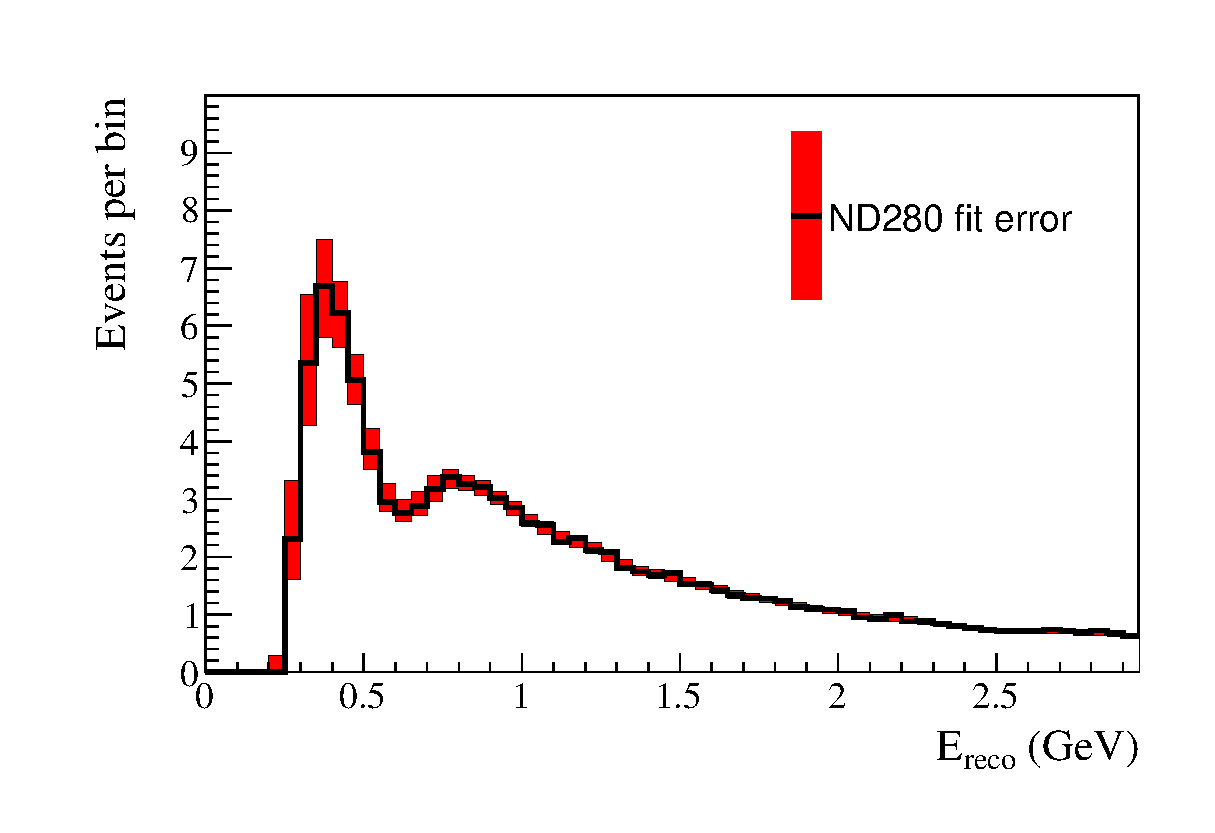
\includegraphics[width=0.9\textwidth]{joint_plots/systematics/Asimov_A_1Rmuoscillated_all_envelope.eps} 
\caption{Muon-like, neutrino mode}
\end{subfigure}
\begin{subfigure}[b]{0.49\textwidth} \centering
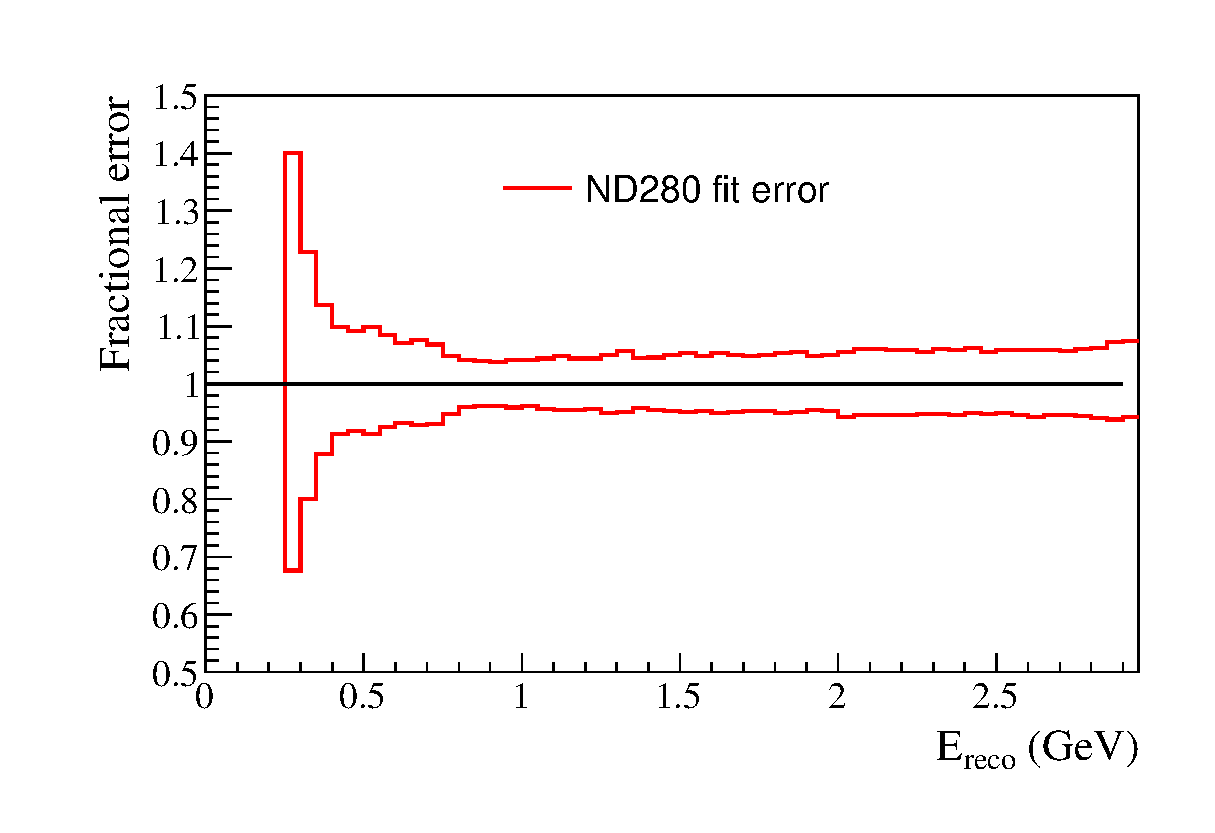
\includegraphics[width=0.9\textwidth]{joint_plots/systematics/Asimov_A_1Rmuoscillated_all_envelope_ratio.eps} \\
\caption{Muon-like, neutrino mode}
\end{subfigure}
%rhc mu-like
\begin{subfigure}[b]{0.49\textwidth} \centering
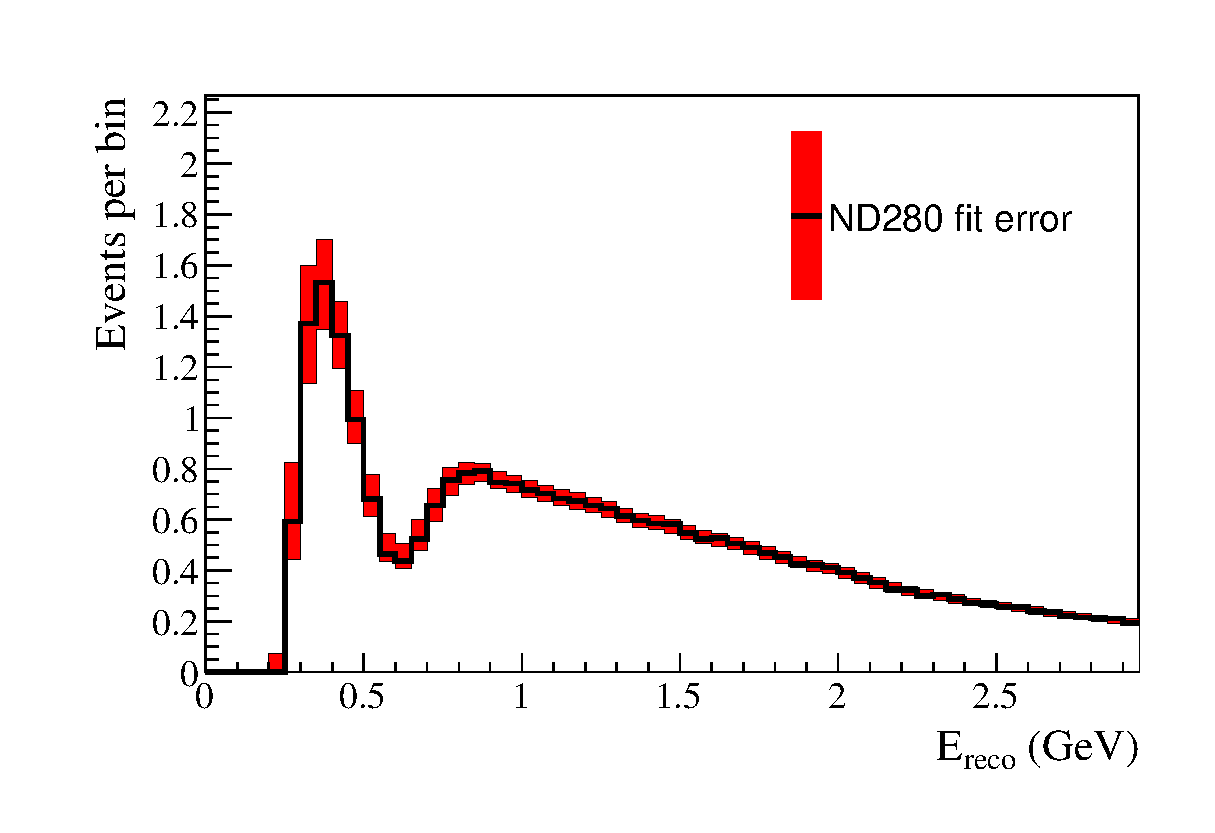
\includegraphics[width=0.9\textwidth]{joint_plots/systematics/Asimov_A_RHC1Rmuoscillated_all_envelope.eps} %\\ 
\caption{Muon-like, antineutrino mode}
\end{subfigure}
\begin{subfigure}[b]{0.49\textwidth} \centering
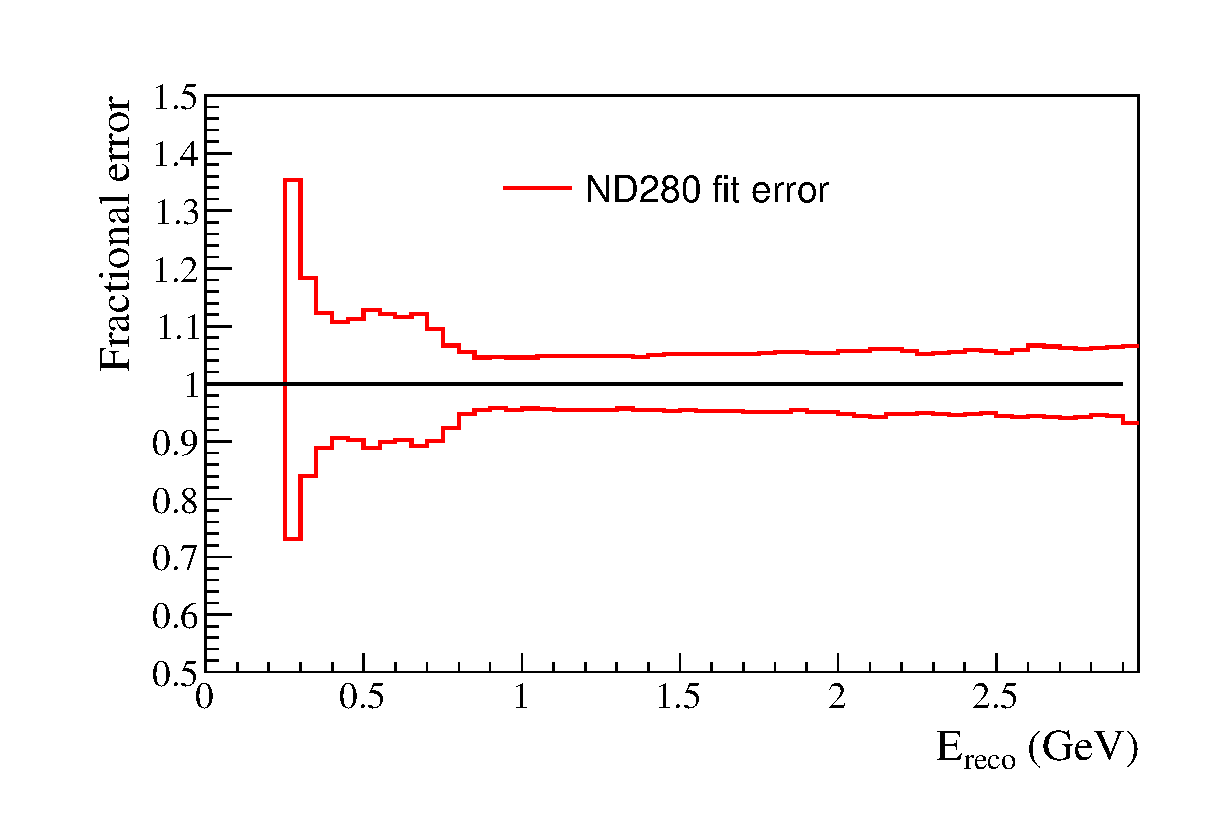
\includegraphics[width=0.9\textwidth]{joint_plots/systematics/Asimov_A_RHC1Rmuoscillated_all_envelope_ratio.eps} \\ 
\caption{Muon-like, antineutrino mode}
\end{subfigure}
%fhc e-like
\begin{subfigure}[b]{0.49\textwidth} \centering
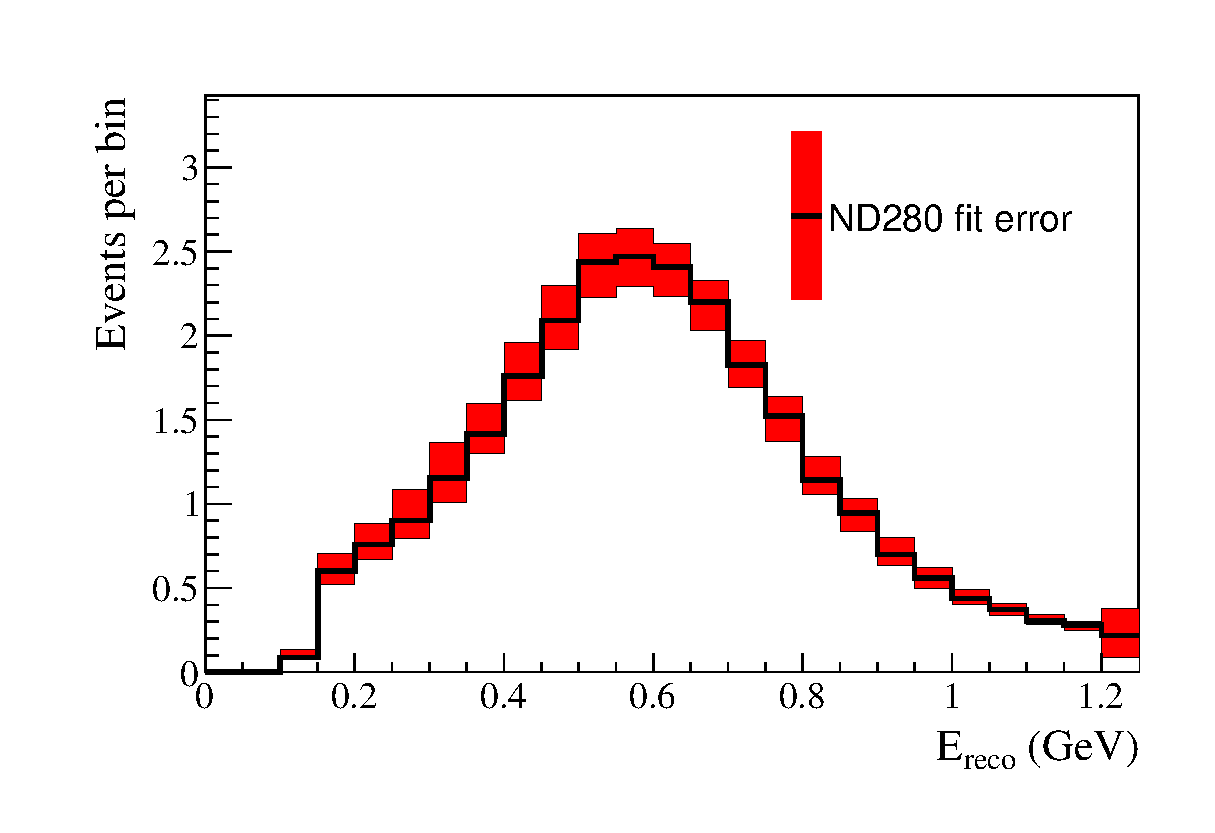
\includegraphics[width=0.9\textwidth]{joint_plots/systematics/Asimov_A_1Reoscillated_all_envelope.eps} 
\caption{Electron-like, neutrino mode}
\end{subfigure}
\begin{subfigure}[b]{0.49\textwidth} \centering
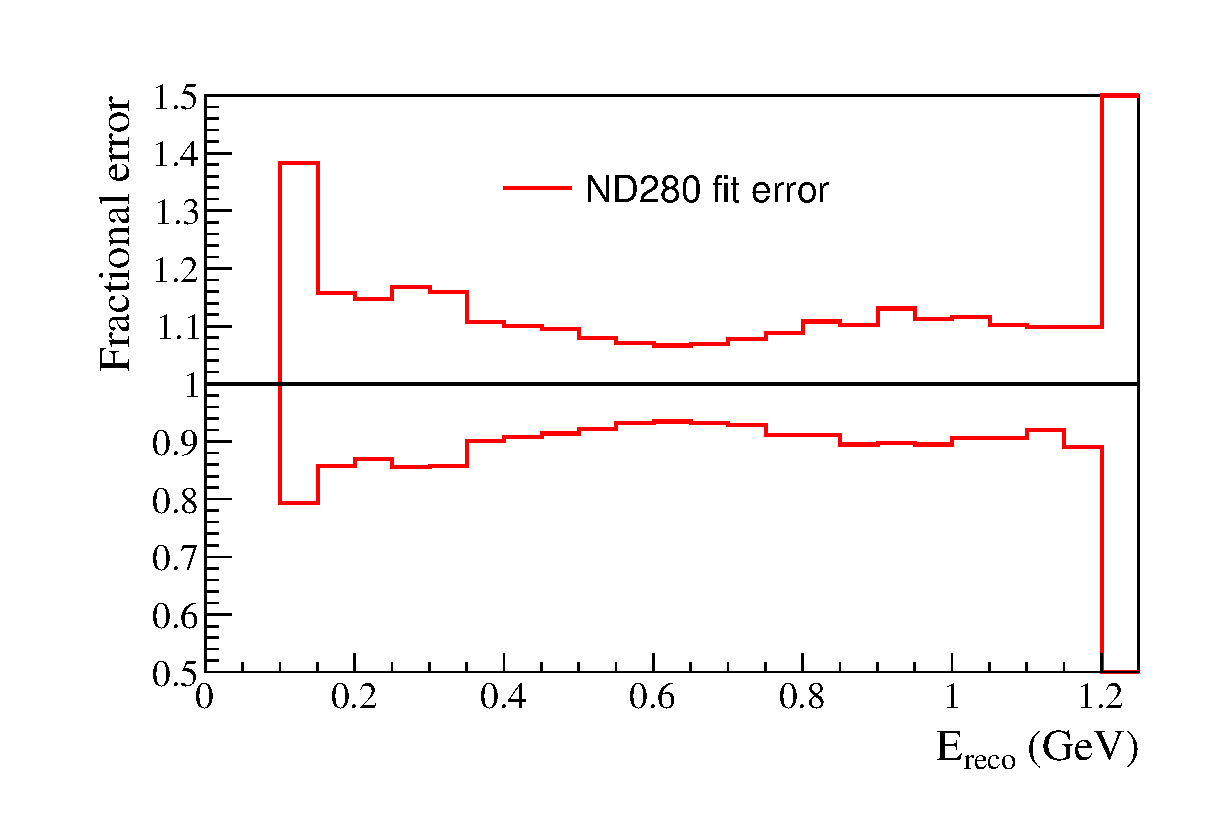
\includegraphics[width=0.9\textwidth]{joint_plots/systematics/Asimov_A_1Reoscillated_all_envelope_ratio.eps} 
\caption{Electron-like, neutrino mode}
\end{subfigure}
%rhc e-like
\begin{subfigure}[b]{0.49\textwidth} \centering
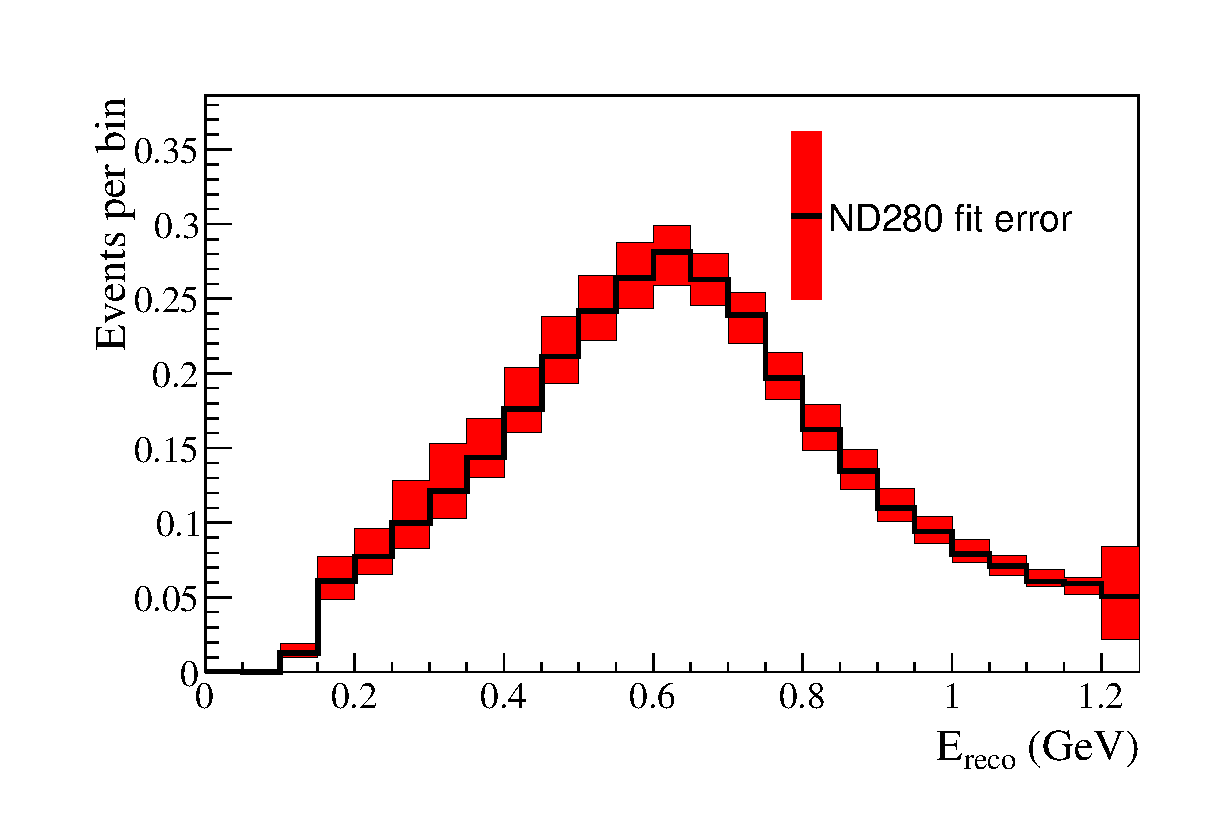
\includegraphics[width=0.9\textwidth]{joint_plots/systematics/Asimov_A_RHC1Reoscillated_all_envelope.eps} 
\caption{Electron-like, antineutrino mode}
\end{subfigure}
\begin{subfigure}[b]{0.49\textwidth} \centering
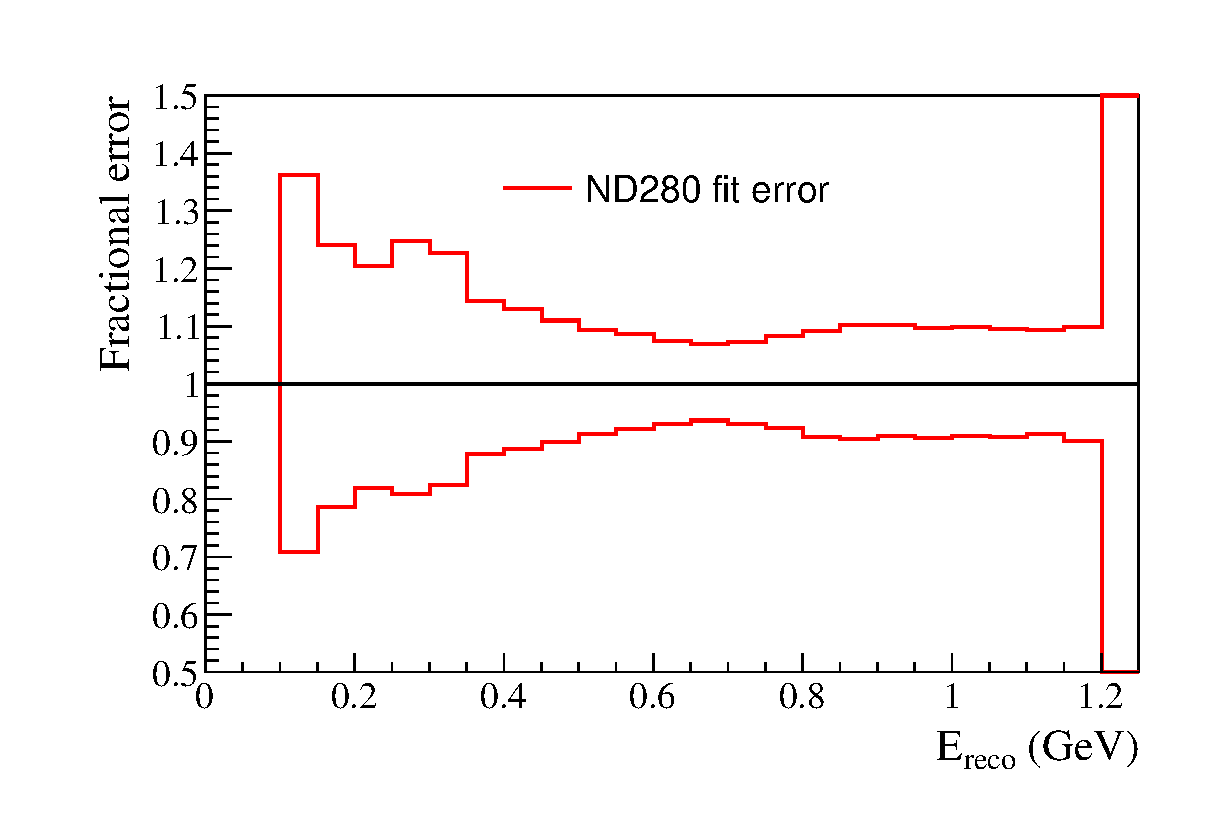
\includegraphics[width=0.9\textwidth]{joint_plots/systematics/Asimov_A_RHC1Reoscillated_all_envelope_ratio.eps} 
\caption{Electron-like, antineutrino mode}
\end{subfigure}
\caption {
Error envelopes (left) and fractional errors (right) for the reconstructed neutrino energy spectrum
for all the systematic parameters.
10k toy MC experiments are generated for the Asimov data set A shown in \cref{tab:osc_params_joint_asimov}
with randomized systematic parameters, taking into account their correlations.
Since the parameters $\delta_{CP}$, $\theta_{23}$ and $\Delta m^2_{32}$ ($\Delta m^2_{13}$) and mass hierarchy
will be measured,
only the uncertainty on 
$\sin^2 \theta_{13}$,
$\sin^2 \theta_{12}$
and 
$\Delta m^2_{21}$ 
are taken into account.
BANFF tuned MC templates are used. 
The distributions correspond to the collected statistics in the full Run 1-6 data set.
}
\label{fig:spectra_systematic_Asimov_A}
\end{figure*}


%%%% Single systematic sources of Asimov A


\begin{figure*}[htb]
\center
%fhc mu-like
\begin{subfigure}[b]{0.49\textwidth} \centering
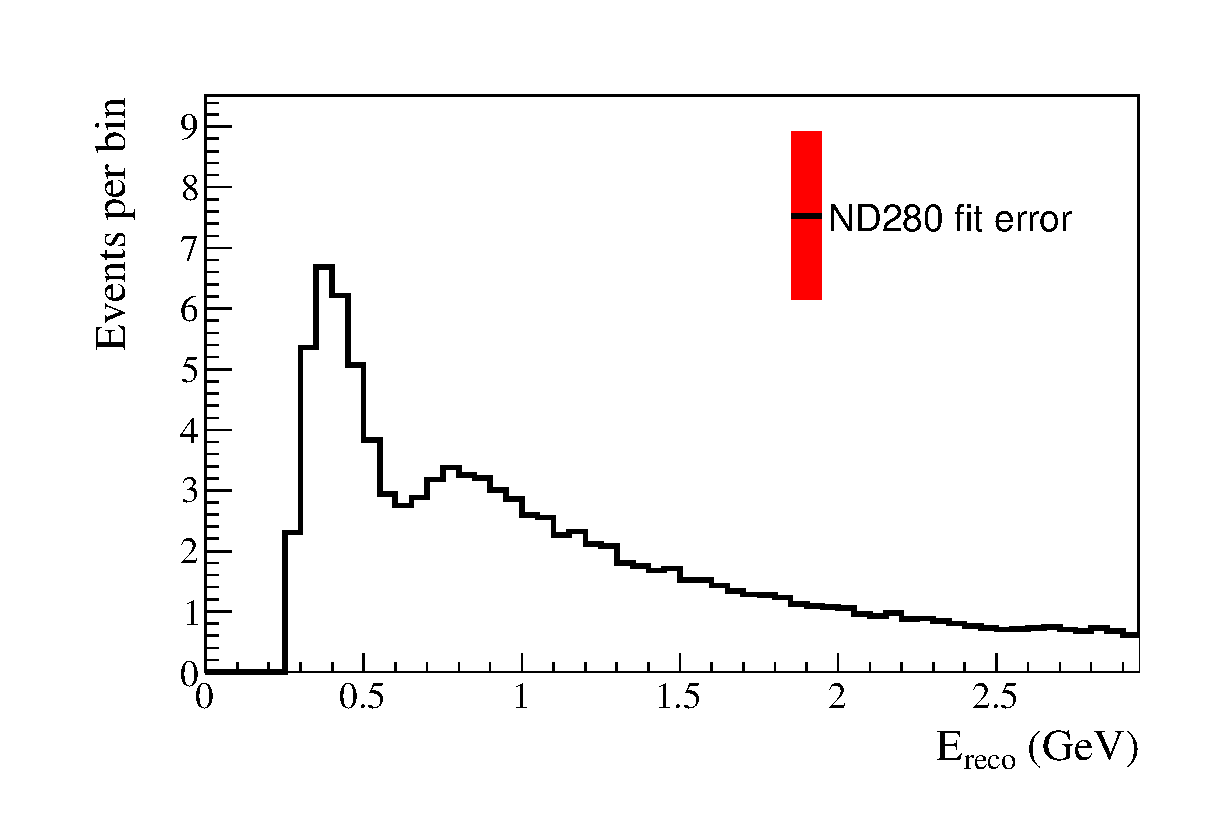
\includegraphics[width=0.9\textwidth]{joint_plots/systematics/Asimov_A_1Rmuoscillated_Osc_param_envelope.eps}
\caption{Muon-like, neutrino mode}
\end{subfigure}
\begin{subfigure}[b]{0.49\textwidth} \centering
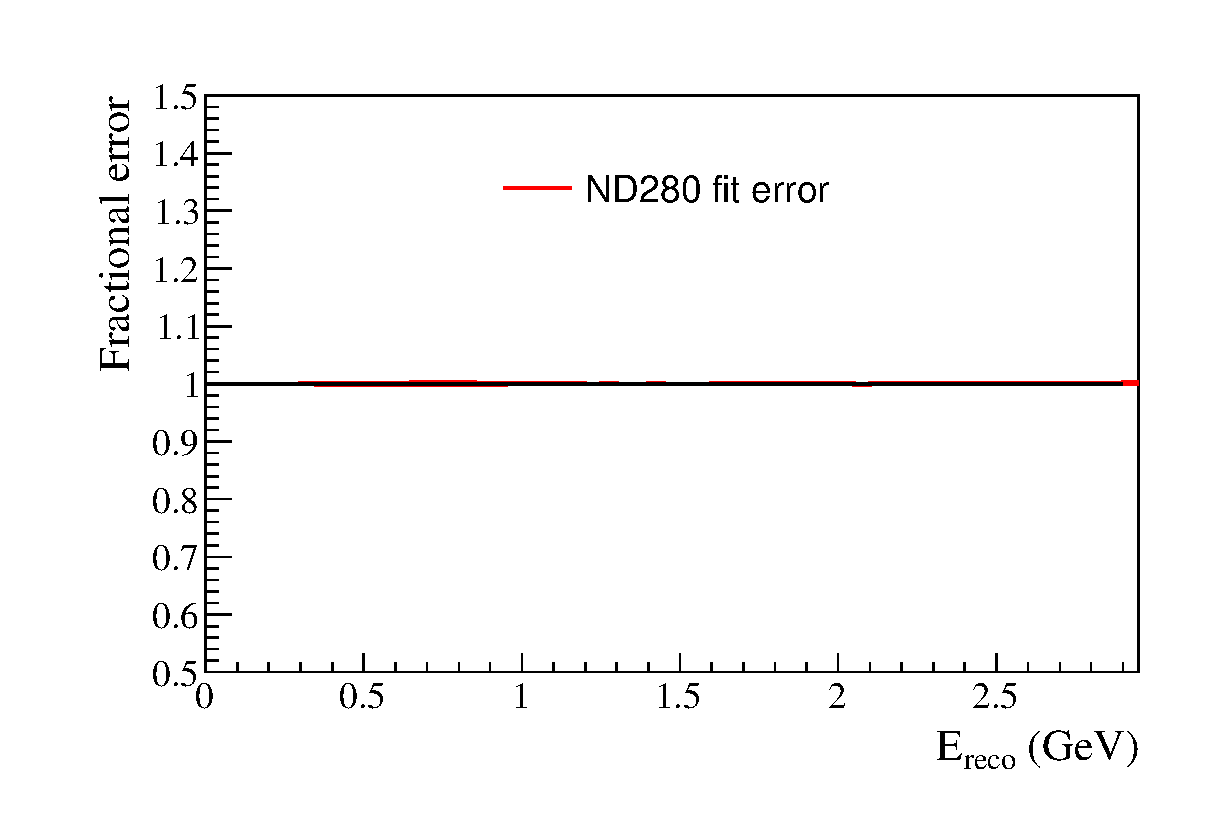
\includegraphics[width=0.9\textwidth]{joint_plots/systematics/Asimov_A_1Rmuoscillated_Osc_param_envelope_ratio.eps} 
\caption{Muon-like, neutrino mode}
\end{subfigure}
%rhc mu-like
\begin{subfigure}[b]{0.49\textwidth} \centering
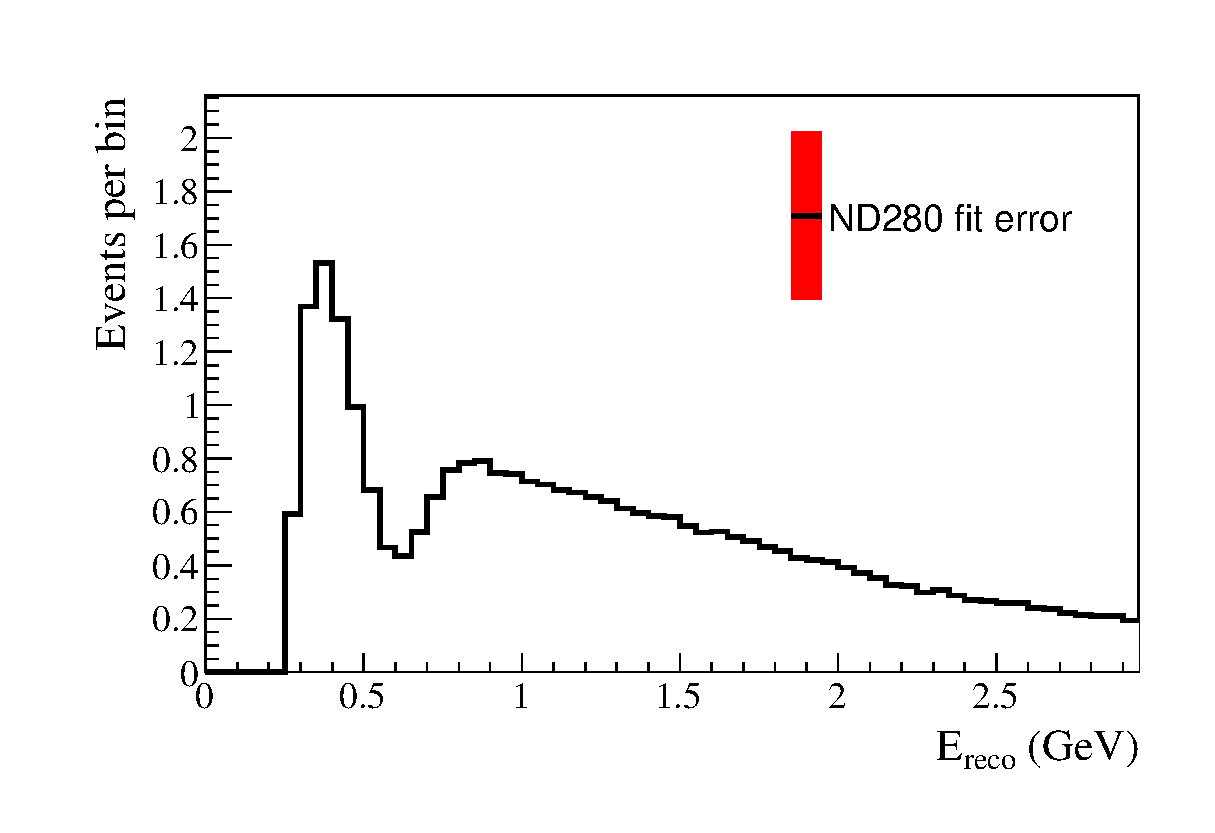
\includegraphics[width=0.9\textwidth]{joint_plots/systematics/Asimov_A_RHC1Rmuoscillated_Osc_param_envelope.eps} \\ 
\caption{Muon-like, antineutrino mode}
\end{subfigure}
\begin{subfigure}[b]{0.49\textwidth} \centering
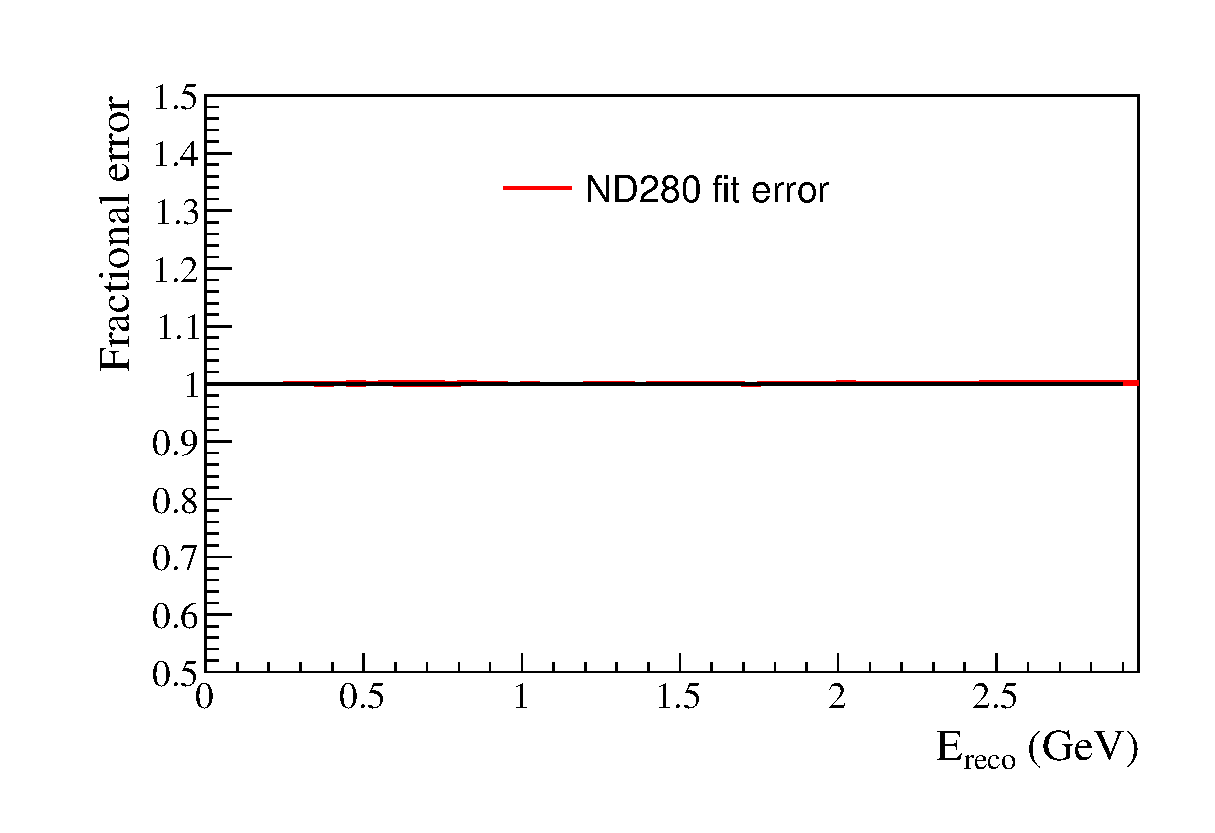
\includegraphics[width=0.9\textwidth]{joint_plots/systematics/Asimov_A_RHC1Rmuoscillated_Osc_param_envelope_ratio.eps} \\ 
\caption{Muon-like, antineutrino mode}
\end{subfigure}
%fhc e-like
\begin{subfigure}[b]{0.49\textwidth} \centering
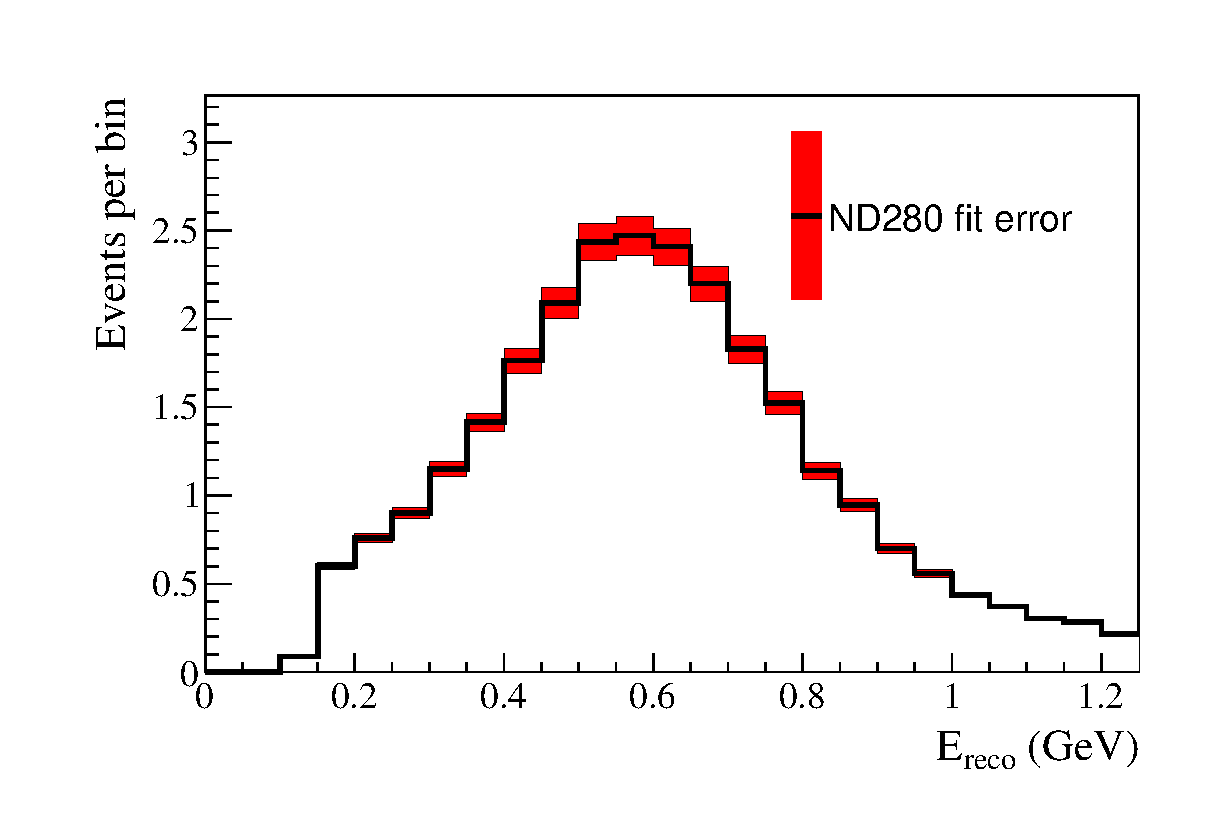
\includegraphics[width=0.9\textwidth]{joint_plots/systematics/Asimov_A_1Reoscillated_Osc_param_envelope.eps} 
\caption{Electron-like, neutrino mode}
\end{subfigure}
\begin{subfigure}[b]{0.49\textwidth} \centering
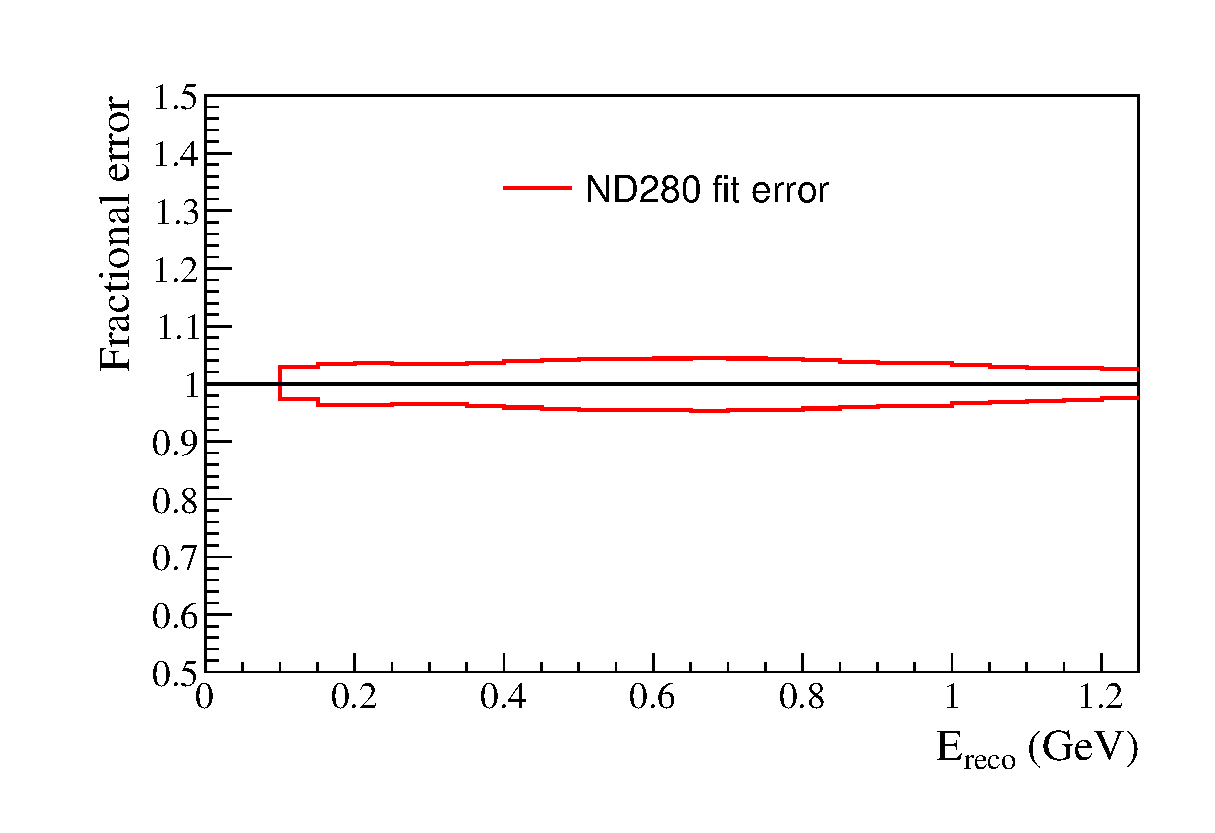
\includegraphics[width=0.9\textwidth]{joint_plots/systematics/Asimov_A_1Reoscillated_Osc_param_envelope_ratio.eps}
\caption{Electron-like, neutrino mode}
\end{subfigure}
%rhc e-like
\begin{subfigure}[b]{0.49\textwidth} \centering
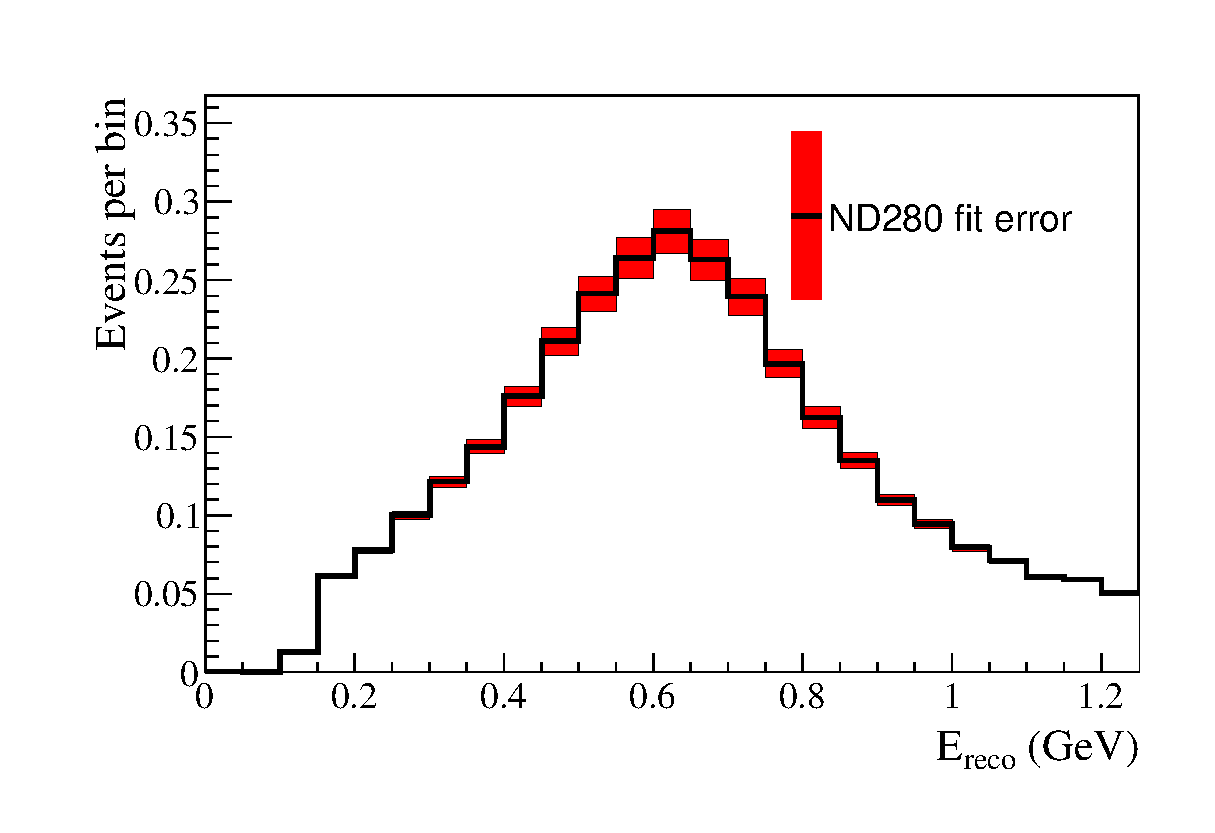
\includegraphics[width=0.9\textwidth]{joint_plots/systematics/Asimov_A_RHC1Reoscillated_Osc_param_envelope.eps}
\caption{Electron-like, antineutrino mode}
\end{subfigure}
\begin{subfigure}[b]{0.49\textwidth} \centering
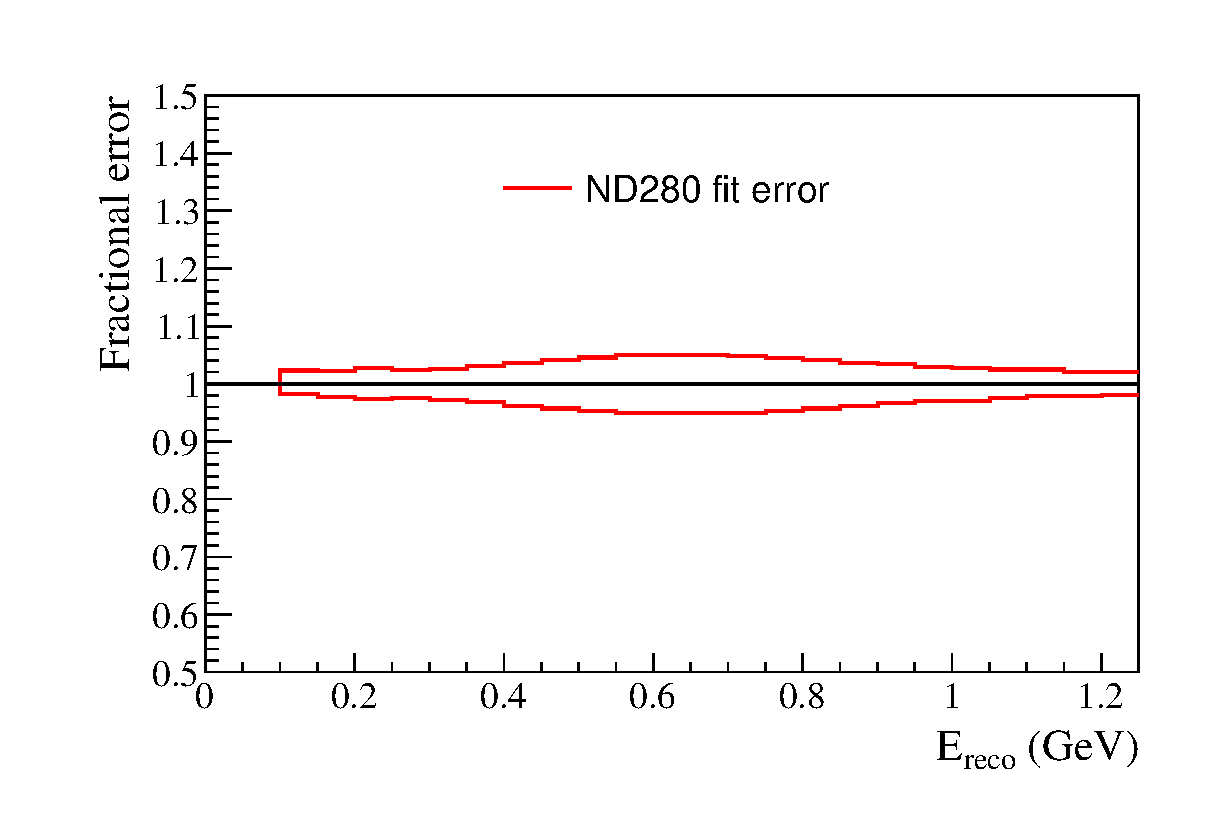
\includegraphics[width=0.9\textwidth]{joint_plots/systematics/Asimov_A_RHC1Reoscillated_Osc_param_envelope_ratio.eps} 
\caption{Electron-like, antineutrino mode}
\end{subfigure}
\caption {
Error envelopes (left) and fractional errors (right) for the reconstructed neutrino energy spectrum
as a result of the oscillation systematic parameters.
10k toy MC experiments are generated for the Asimov data set A shown in \cref{tab:osc_params_joint_asimov}
with randomized systematic parameters, taking into account their correlations.
Since the parameters $\delta_{CP}$, $\theta_{23}$ and $\Delta m^2_{32}$ ($\Delta m^2_{13}$) and mass hierarchy
will be measured,
only the uncertainty on 
$\sin^2 \theta_{13}$,
$\sin^2 \theta_{12}$
and 
$\Delta m^2_{21}$ 
are taken into account.
BANFF tuned MC templates are used. 
The distributions correspond to the collected statistics in the full Run 1-6 data set.
}
\label{fig:Osc_envelope_Asimov_A}
\end{figure*}


\begin{figure*}[htb]
\center
%fhc mu-like
\begin{subfigure}[b]{0.49\textwidth} \centering
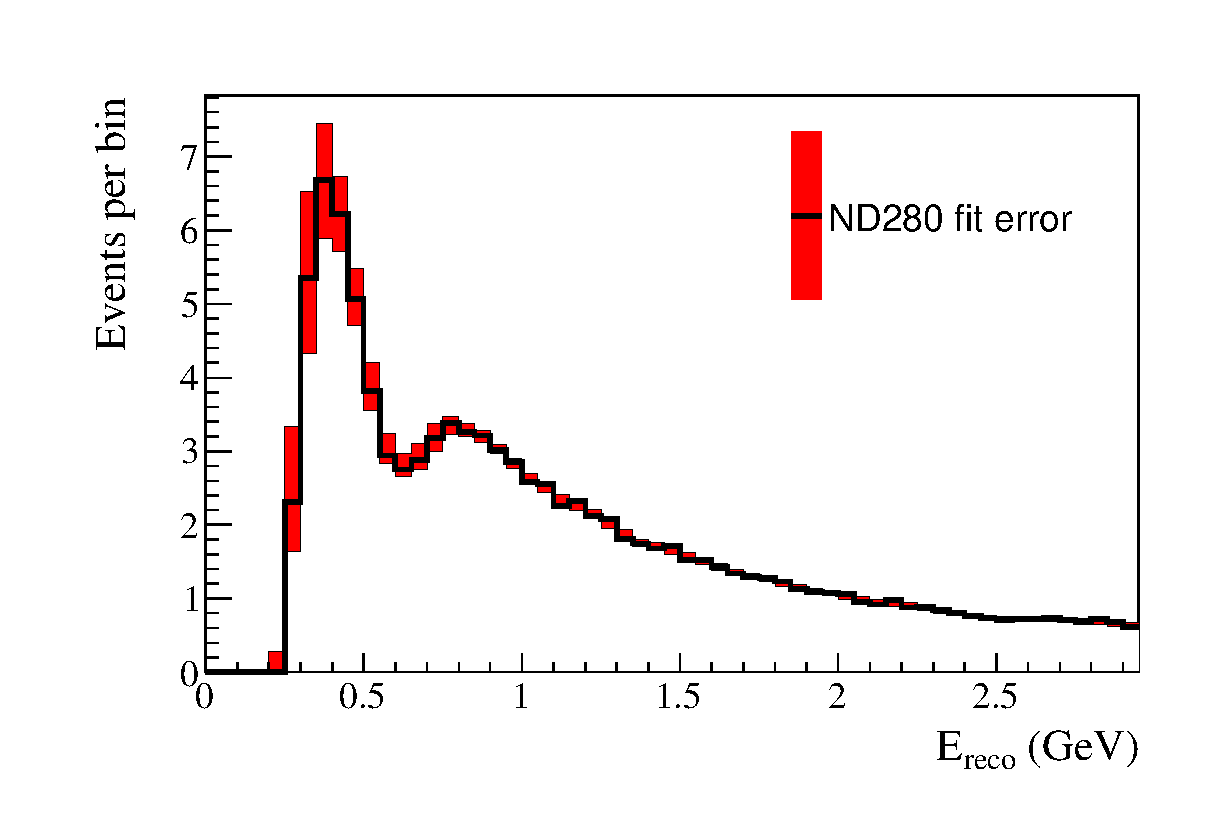
\includegraphics[width=0.9\textwidth]{joint_plots/systematics/Asimov_A_1Rmuoscillated_SKDet_FSI_envelope.eps} 
\caption{Muon-like, neutrino mode}
\end{subfigure}
\begin{subfigure}[b]{0.49\textwidth} \centering
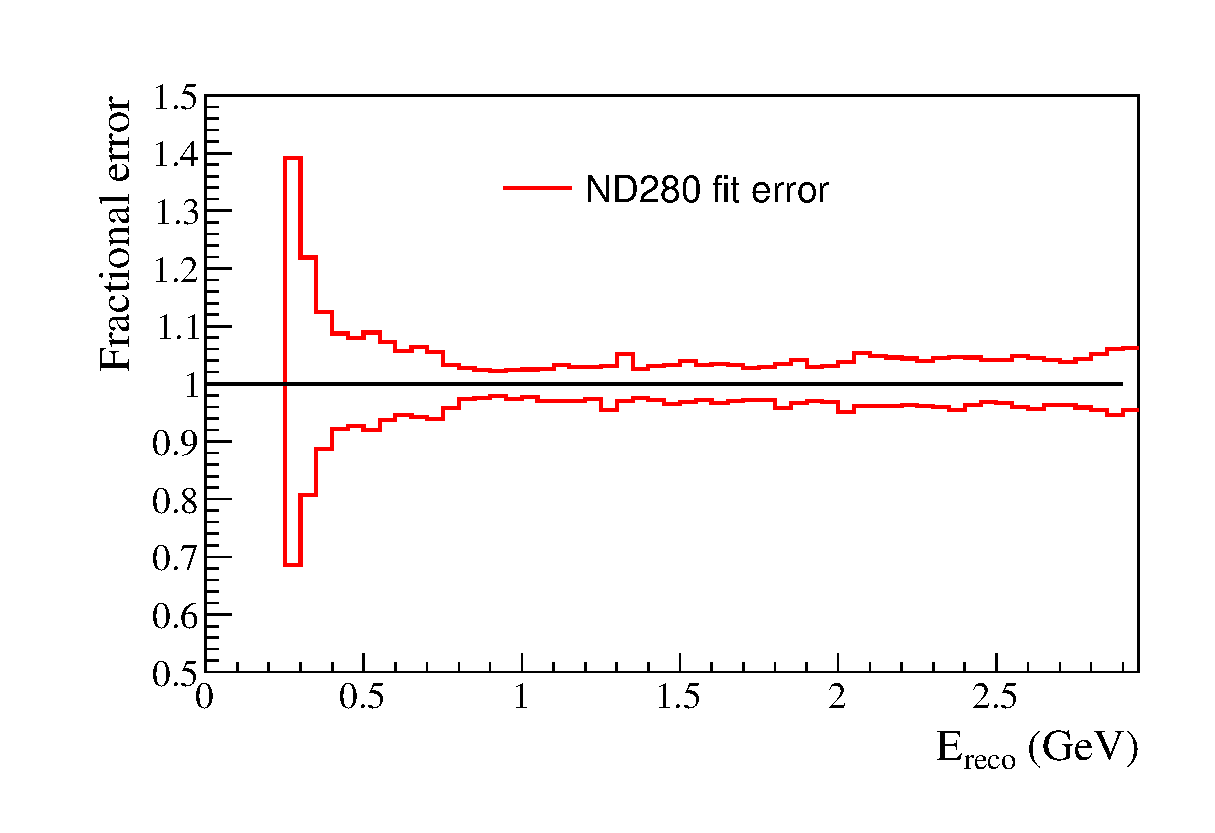
\includegraphics[width=0.9\textwidth]{joint_plots/systematics/Asimov_A_1Rmuoscillated_SKDet_FSI_envelope_ratio.eps} 
\caption{Muon-like, neutrino mode}
\end{subfigure}
%rhc mu-like
\begin{subfigure}[b]{0.49\textwidth} \centering
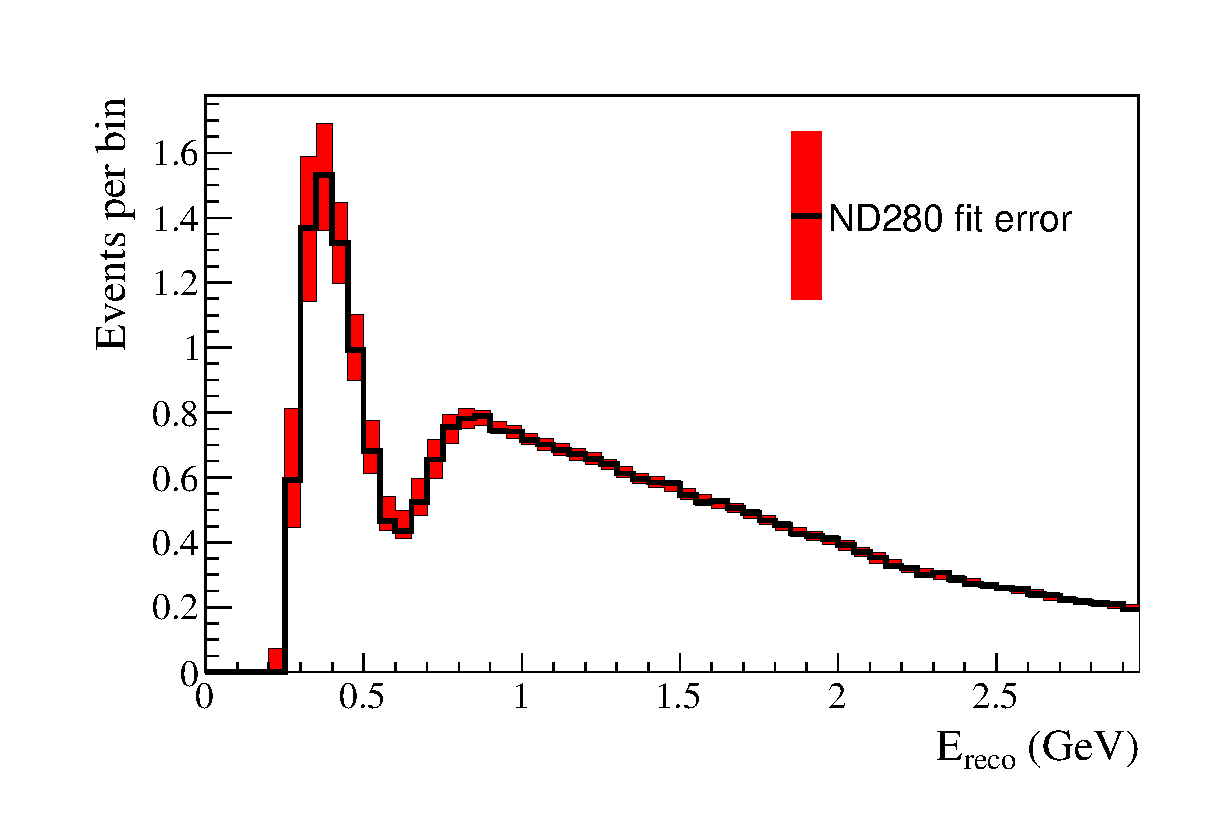
\includegraphics[width=0.9\textwidth]{joint_plots/systematics/Asimov_A_RHC1Rmuoscillated_SKDet_FSI_envelope.eps} \\ 
\caption{Muon-like, antineutrino mode}
\end{subfigure}
\begin{subfigure}[b]{0.49\textwidth} \centering
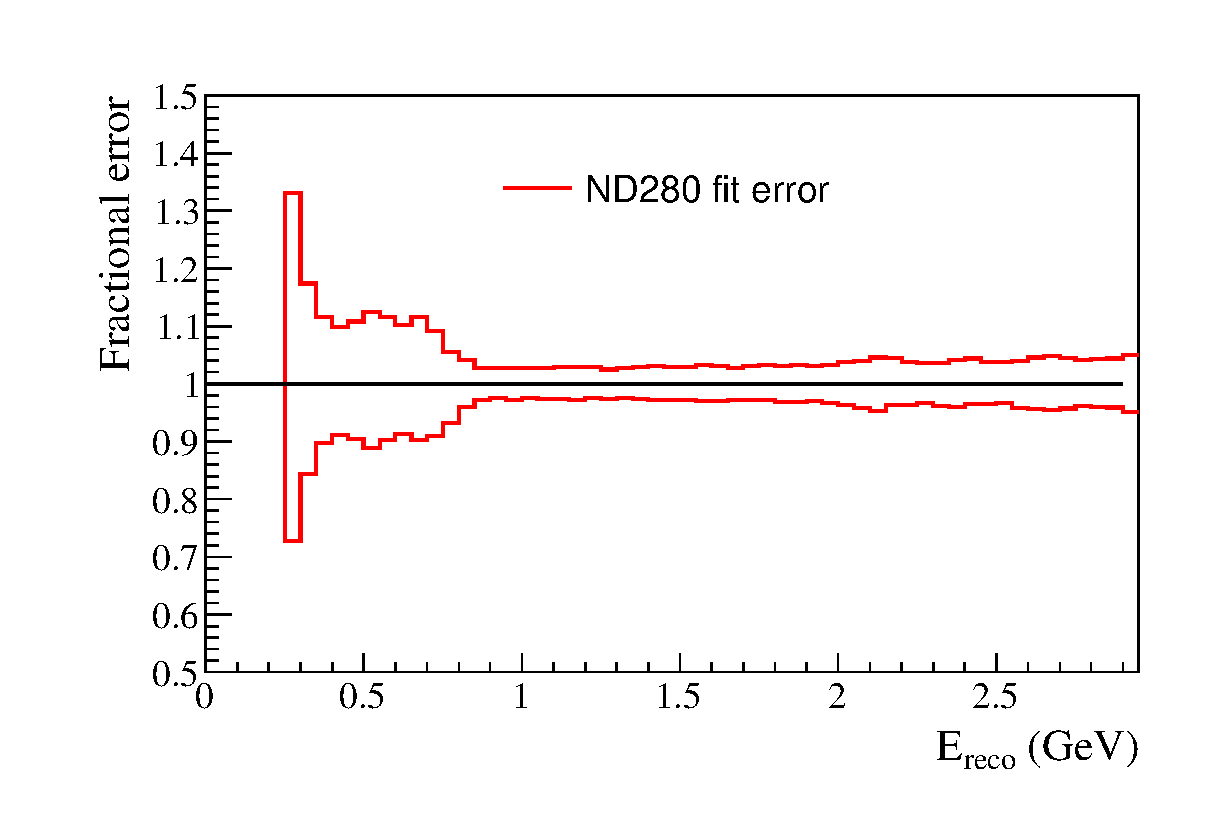
\includegraphics[width=0.9\textwidth]{joint_plots/systematics/Asimov_A_RHC1Rmuoscillated_SKDet_FSI_envelope_ratio.eps} \\ 
\caption{Muon-like, antineutrino mode}
\end{subfigure}
%fhc e-like
\begin{subfigure}[b]{0.49\textwidth} \centering
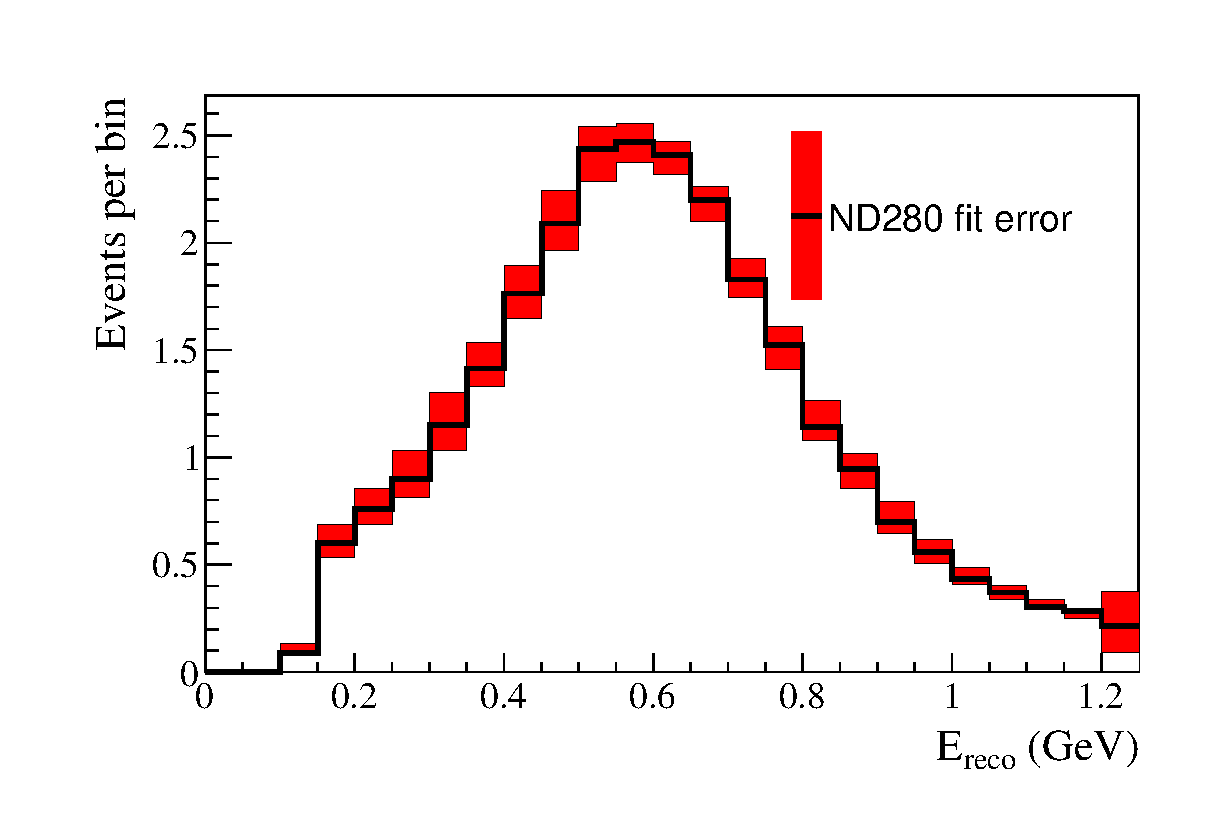
\includegraphics[width=0.9\textwidth]{joint_plots/systematics/Asimov_A_1Reoscillated_SKDet_FSI_envelope.eps} 
\caption{Electron-like, neutrino mode}
\end{subfigure}
\begin{subfigure}[b]{0.49\textwidth} \centering
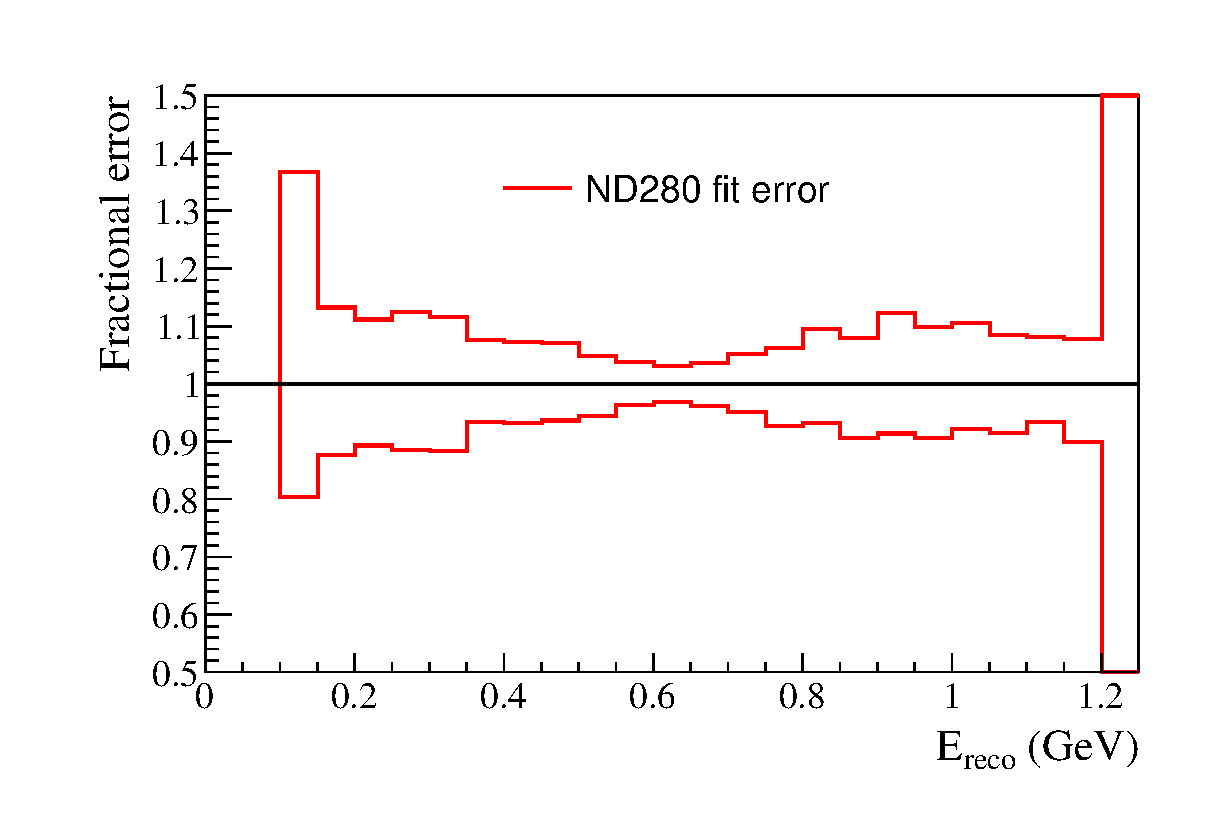
\includegraphics[width=0.9\textwidth]{joint_plots/systematics/Asimov_A_1Reoscillated_SKDet_FSI_envelope_ratio.eps} 
\caption{Electron-like, neutrino mode}
\end{subfigure}
%rhc e-like
\begin{subfigure}[b]{0.49\textwidth} \centering
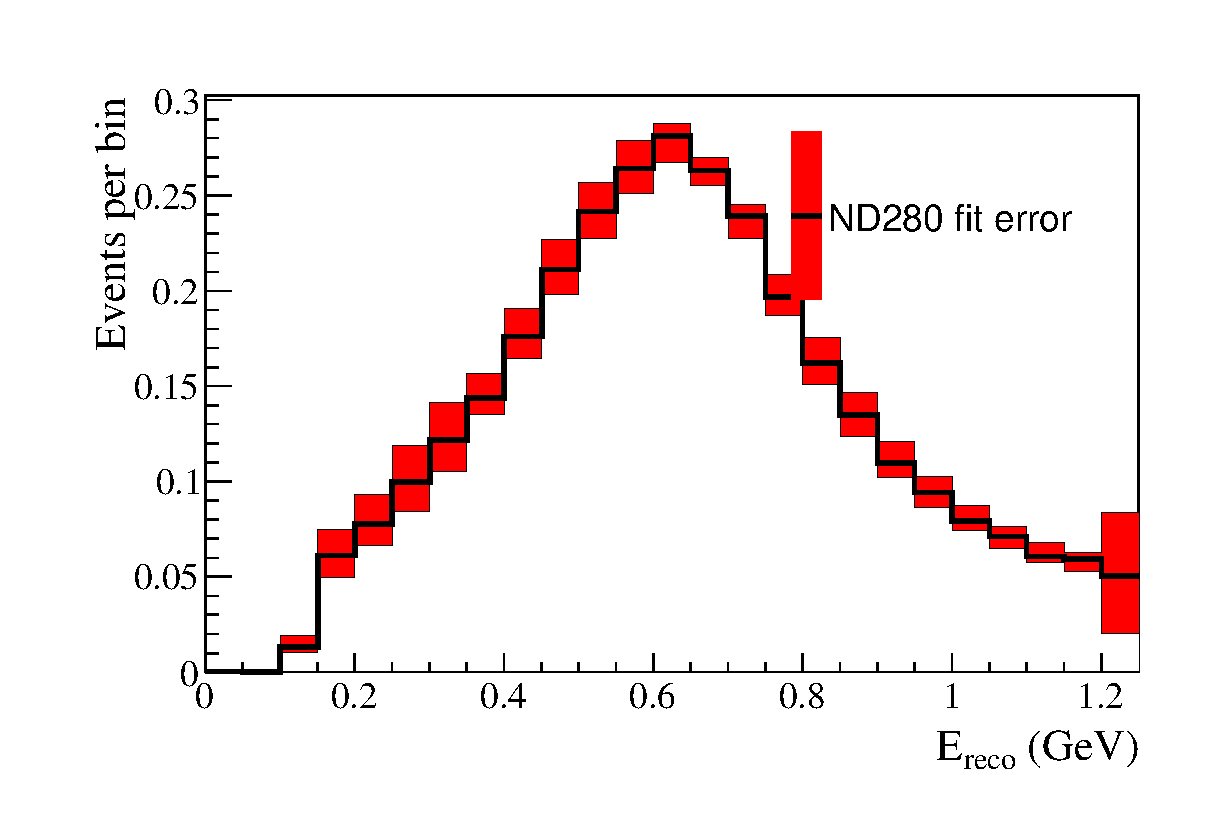
\includegraphics[width=0.9\textwidth]{joint_plots/systematics/Asimov_A_RHC1Reoscillated_SKDet_FSI_envelope.eps} 
\caption{Electron-like, antineutrino mode}
\end{subfigure}
\begin{subfigure}[b]{0.49\textwidth} \centering
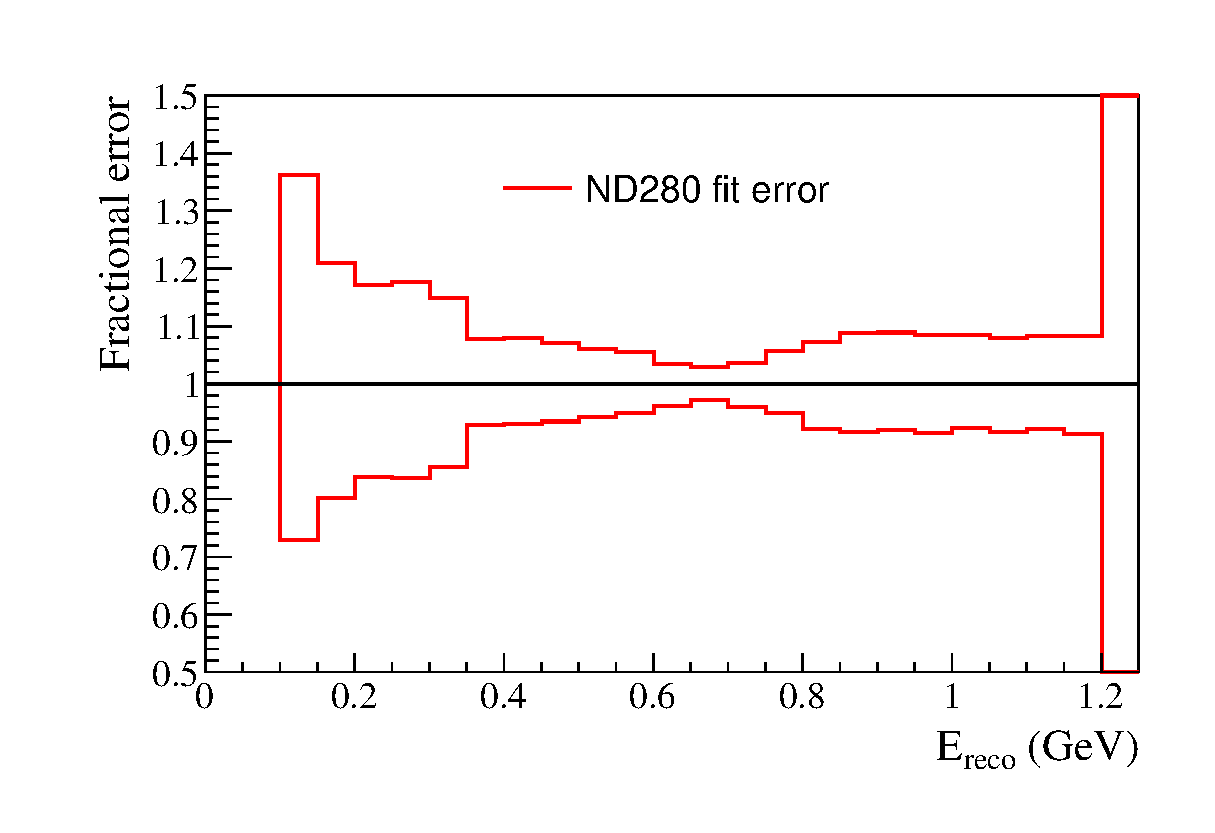
\includegraphics[width=0.9\textwidth]{joint_plots/systematics/Asimov_A_RHC1Reoscillated_SKDet_FSI_envelope_ratio.eps} 
\caption{Electron-like, antineutrino mode}
\end{subfigure}
\caption {
Error envelopes (left) and fractional errors (right) for the reconstructed neutrino energy spectrum
as a result of the Super-K + FSI + SI + PN systematic parameters.
10k toy MC experiments are generated for the Asimov data set A shown in \cref{tab:osc_params_joint_asimov}
with randomized systematic parameters, taking into account their correlations.
Since the parameters $\delta_{CP}$, $\theta_{23}$ and $\Delta m^2_{32}$ ($\Delta m^2_{13}$) and mass hierarchy
will be measured,
only the uncertainty on 
$\sin^2 \theta_{13}$,
$\sin^2 \theta_{12}$
and 
$\Delta m^2_{21}$ 
are taken into account.
BANFF tuned MC templates are used. 
The distributions correspond to the collected statistics in the full Run 1-6 data set.
}
\label{fig:SKDet_FSI_envelope_Asimov_A}
\end{figure*}




\begin{figure*}[htb]
\center
%fhc mu-like
\begin{subfigure}[b]{0.49\textwidth} \centering
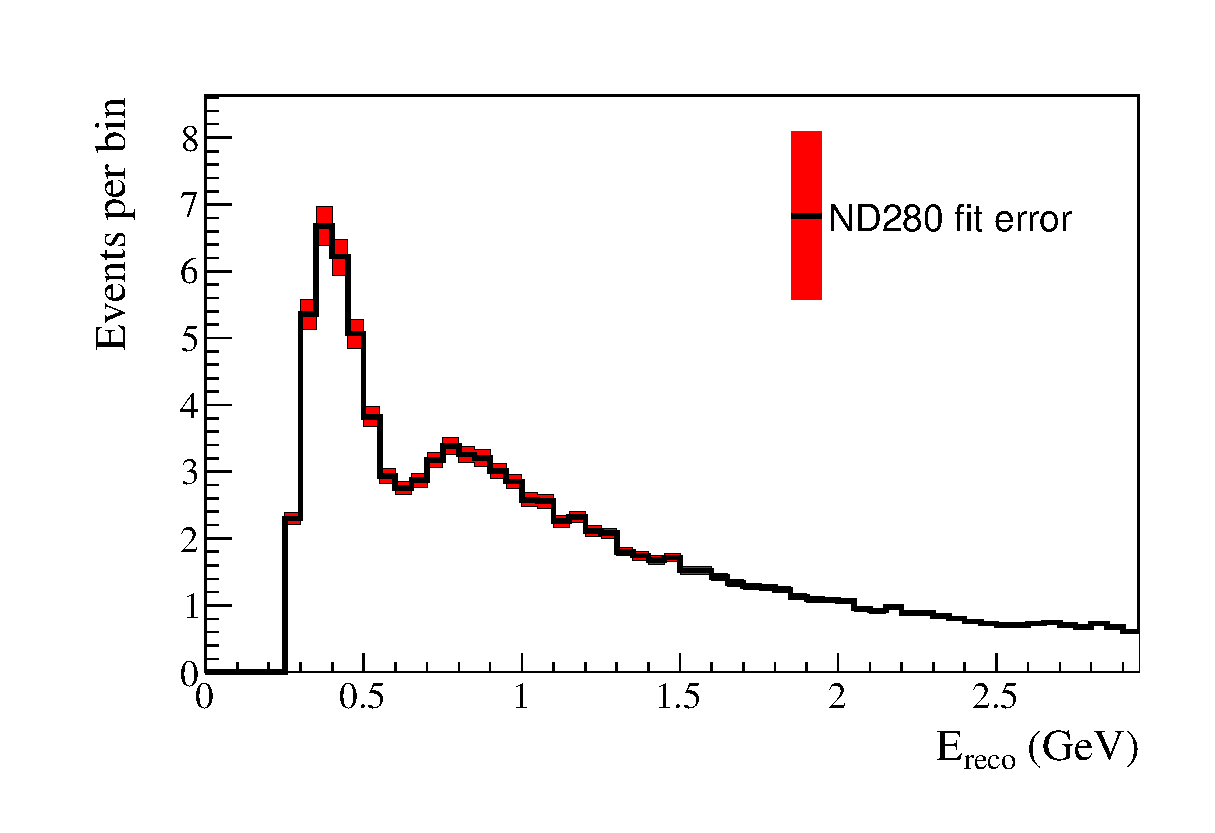
\includegraphics[width=0.9\textwidth]{joint_plots/systematics/Asimov_A_1Rmuoscillated_BANFF_flux_envelope.eps} 
\caption{Muon-like, neutrino mode}
\end{subfigure}
\begin{subfigure}[b]{0.49\textwidth} \centering
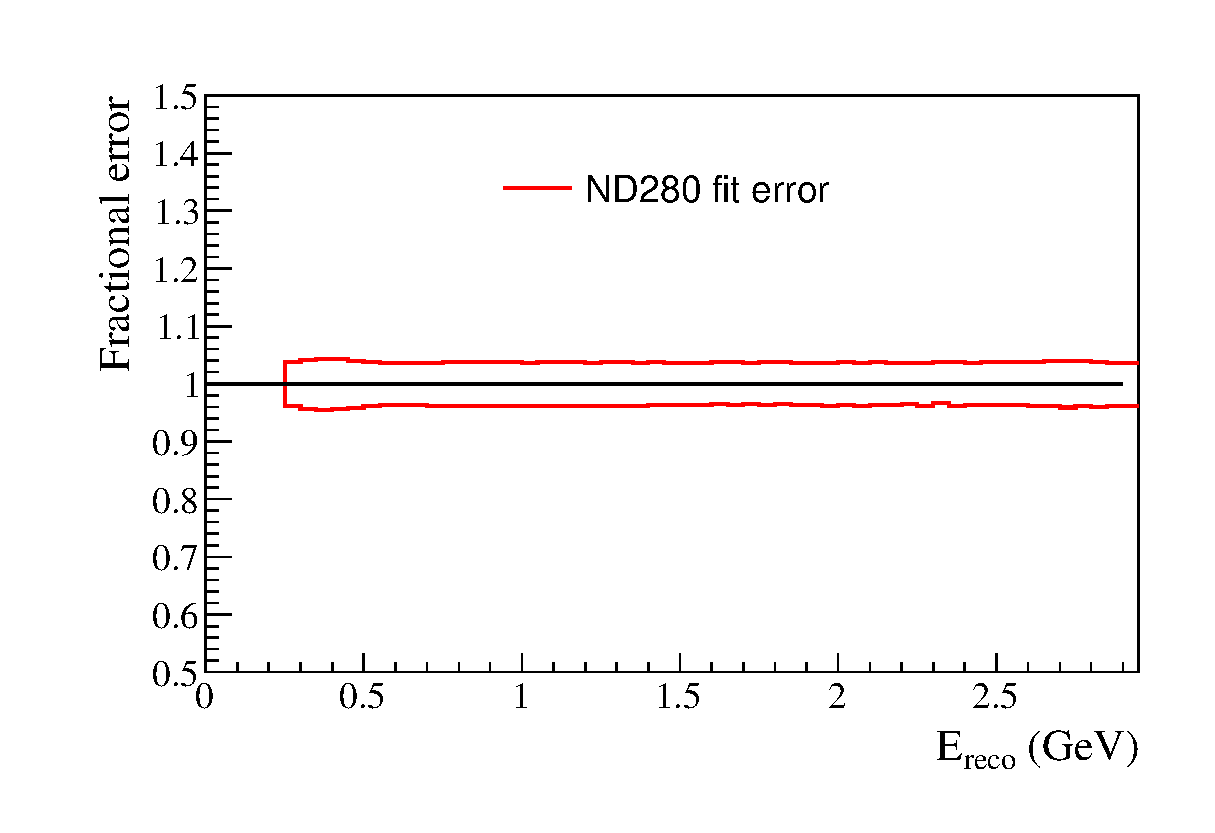
\includegraphics[width=0.9\textwidth]{joint_plots/systematics/Asimov_A_1Rmuoscillated_BANFF_flux_envelope_ratio.eps} 
\caption{Muon-like, neutrino mode}
\end{subfigure}
%rhc mu-like
\begin{subfigure}[b]{0.49\textwidth} \centering
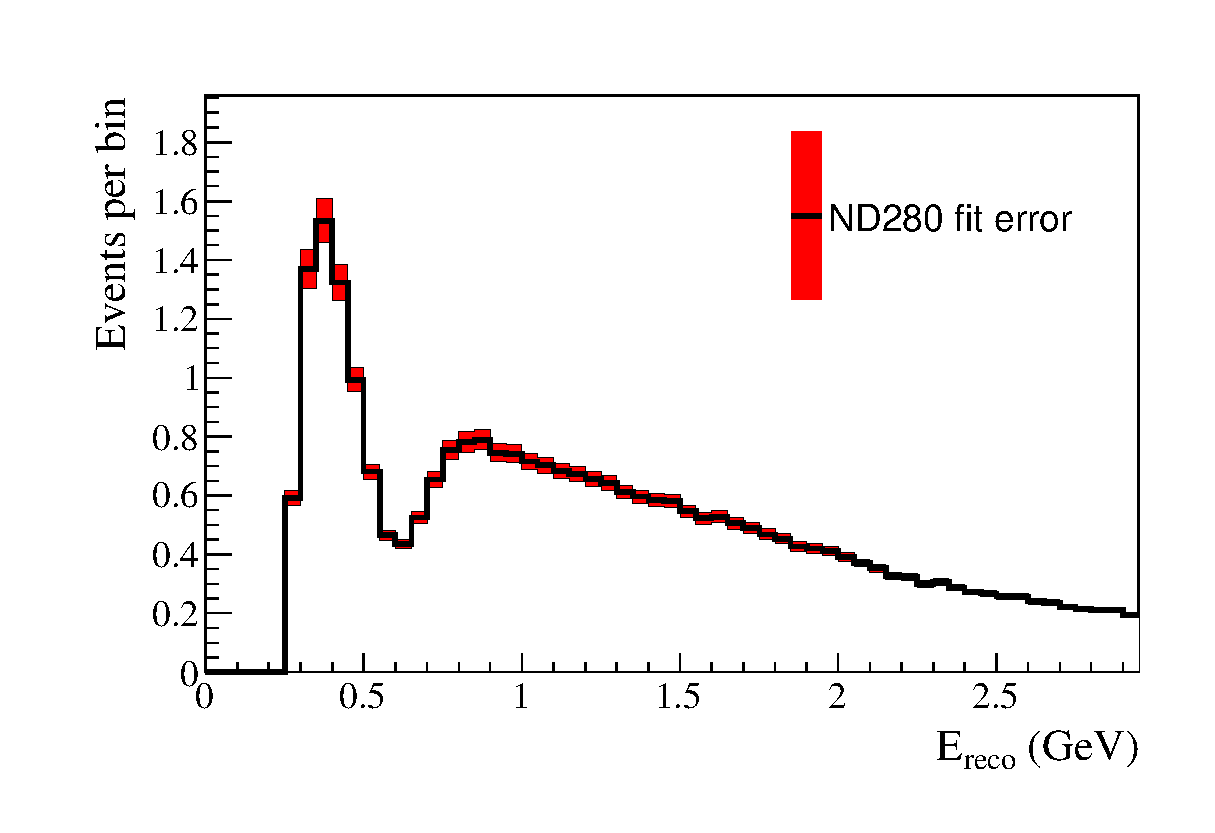
\includegraphics[width=0.9\textwidth]{joint_plots/systematics/Asimov_A_RHC1Rmuoscillated_BANFF_flux_envelope.eps} \\ 
\caption{Muon-like, antineutrino mode}
\end{subfigure}
\begin{subfigure}[b]{0.49\textwidth} \centering
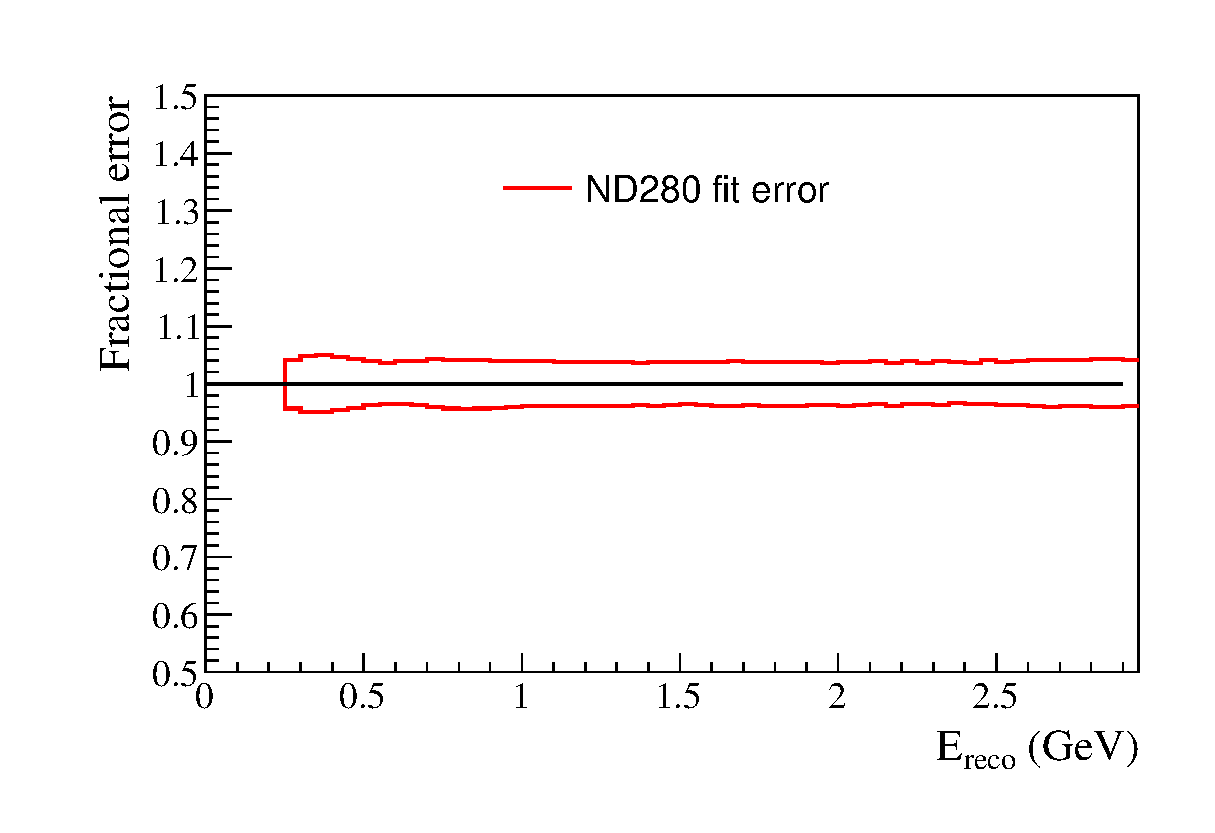
\includegraphics[width=0.9\textwidth]{joint_plots/systematics/Asimov_A_RHC1Rmuoscillated_BANFF_flux_envelope_ratio.eps} \\ 
\caption{Muon-like, antineutrino mode}
\end{subfigure}
%fhc e-like
\begin{subfigure}[b]{0.49\textwidth} \centering
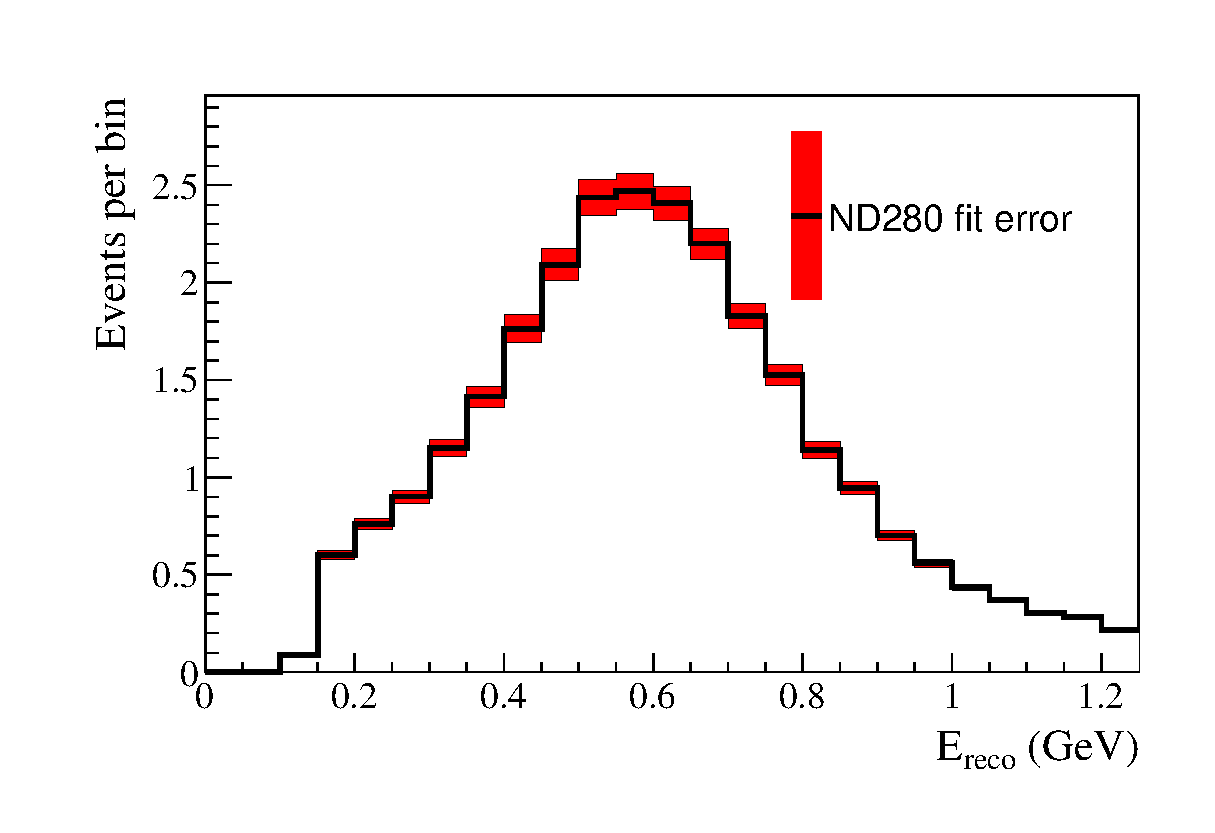
\includegraphics[width=0.9\textwidth]{joint_plots/systematics/Asimov_A_1Reoscillated_BANFF_flux_envelope.eps} 
\caption{Electron-like, neutrino mode}
\end{subfigure}
\begin{subfigure}[b]{0.49\textwidth} \centering
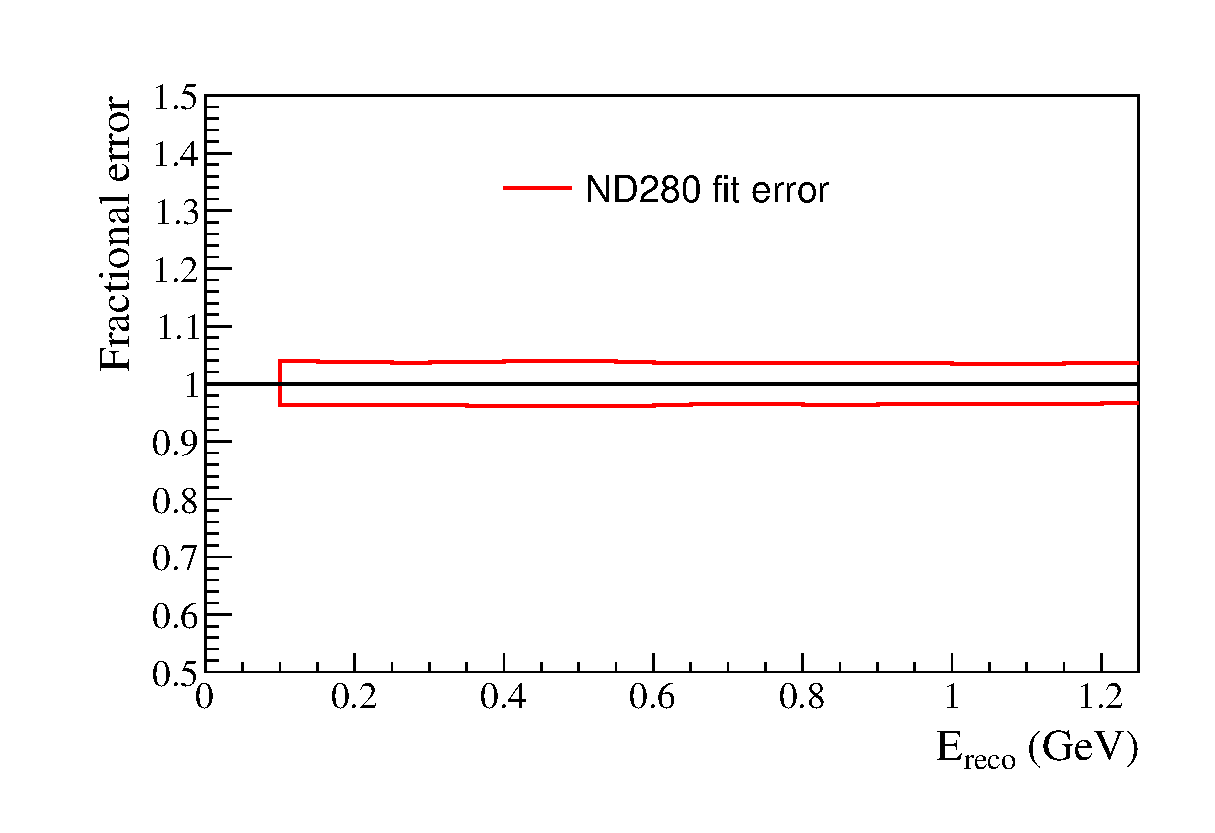
\includegraphics[width=0.9\textwidth]{joint_plots/systematics/Asimov_A_1Reoscillated_BANFF_flux_envelope_ratio.eps} 
\caption{Electron-like, neutrino mode}
\end{subfigure}
%rhc e-like
\begin{subfigure}[b]{0.49\textwidth} \centering
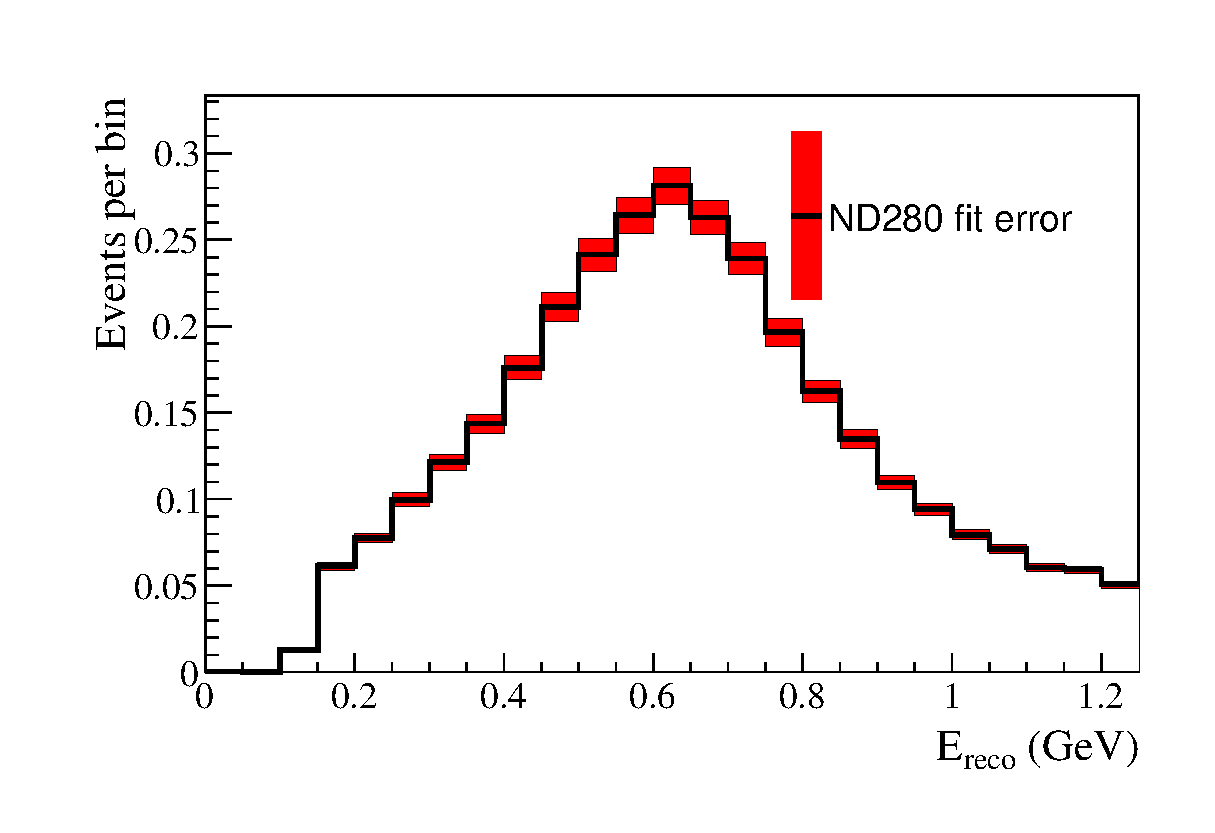
\includegraphics[width=0.9\textwidth]{joint_plots/systematics/Asimov_A_RHC1Reoscillated_BANFF_flux_envelope.eps} 
\caption{Electron-like, antineutrino mode}
\end{subfigure}
\begin{subfigure}[b]{0.49\textwidth} \centering
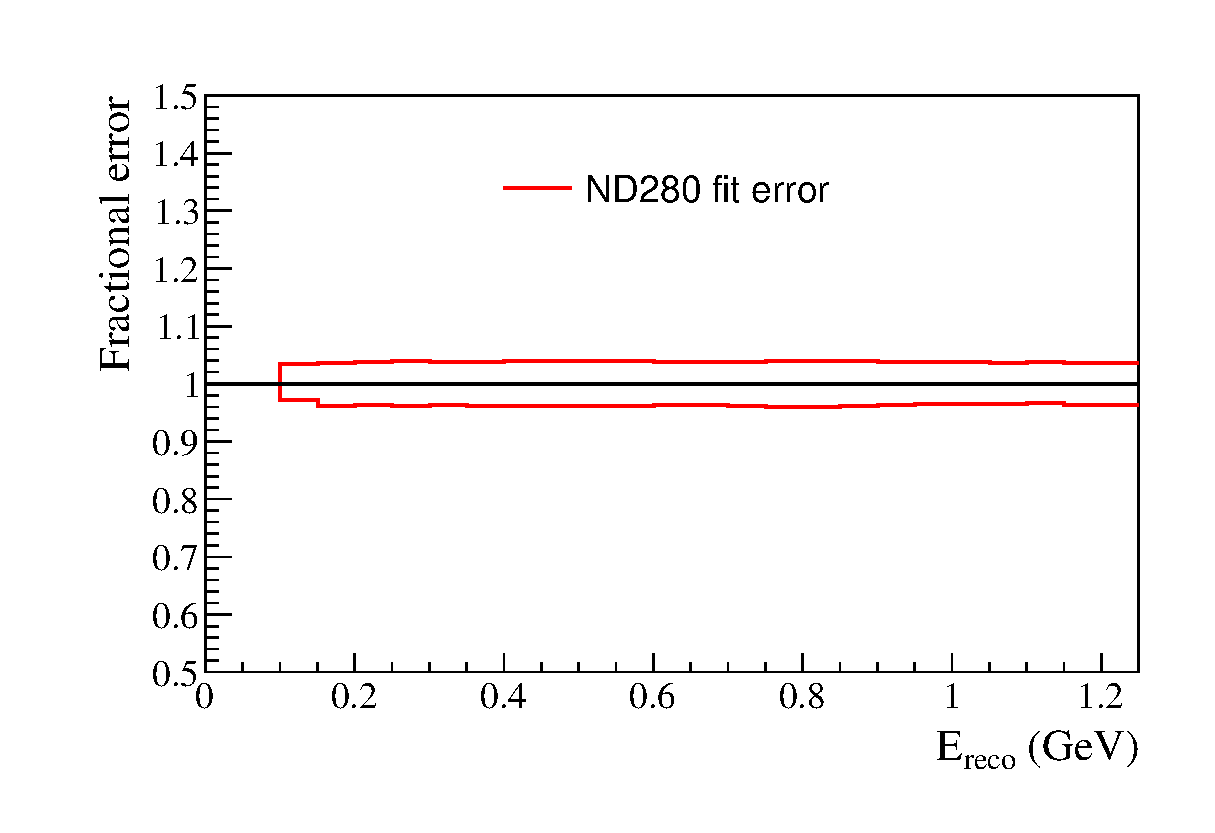
\includegraphics[width=0.9\textwidth]{joint_plots/systematics/Asimov_A_RHC1Reoscillated_BANFF_flux_envelope_ratio.eps} 
\caption{Electron-like, antineutrino mode}
\end{subfigure}
\caption {
Error envelopes (left) and fractional errors (right) for the reconstructed neutrino energy spectrum
as a result of the flux systematic parameters.
10k toy MC experiments are generated for the Asimov data set A shown in \cref{tab:osc_params_joint_asimov}
with randomized systematic parameters, taking into account their correlations.
Since the parameters $\delta_{CP}$, $\theta_{23}$ and $\Delta m^2_{32}$ ($\Delta m^2_{13}$) and mass hierarchy
will be measured,
only the uncertainty on 
$\sin^2 \theta_{13}$,
$\sin^2 \theta_{12}$
and 
$\Delta m^2_{21}$ 
are taken into account.
BANFF tuned MC templates are used. 
The distributions correspond to the collected statistics in the full Run 1-6 data set.
}
\label{fig:flux_envelope_Asimov_A}
\end{figure*}


\begin{figure*}[htb]
\center
%fhc mu-like
\begin{subfigure}[b]{0.49\textwidth} \centering
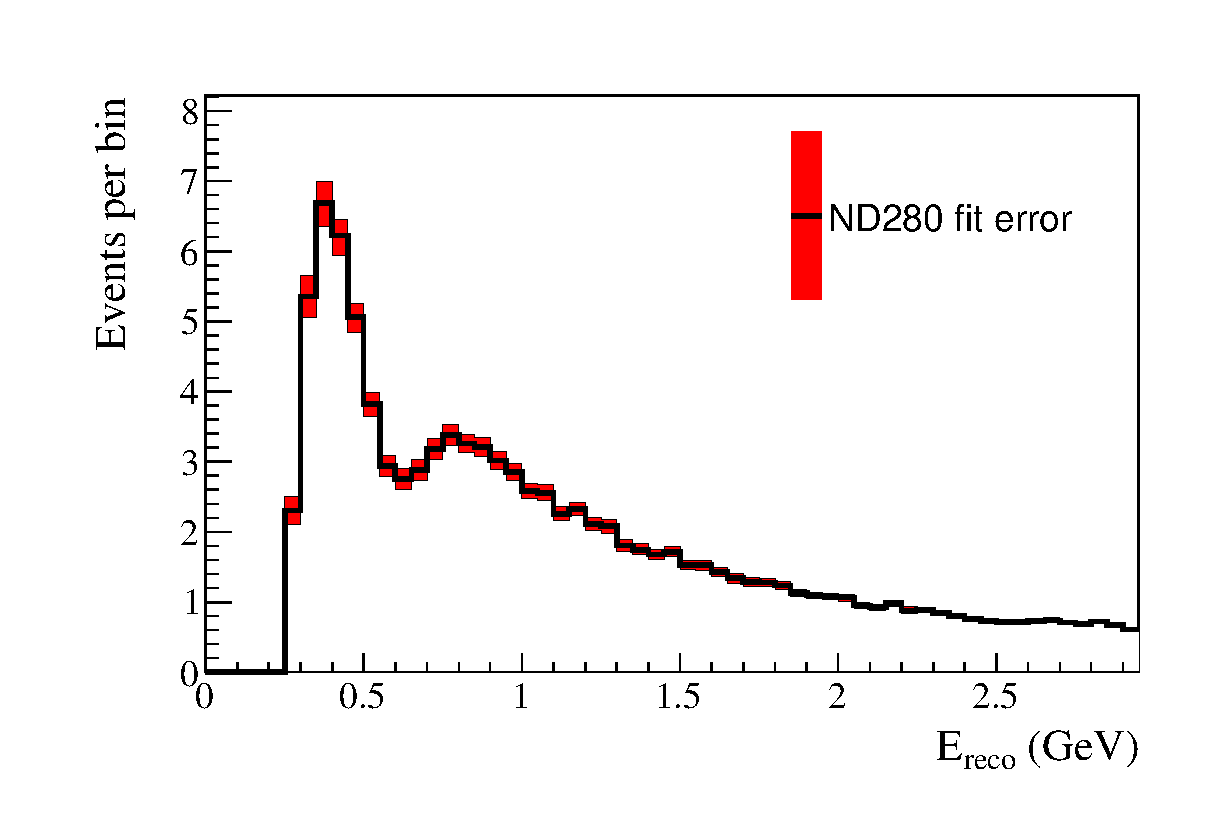
\includegraphics[width=0.9\textwidth]{joint_plots/systematics/Asimov_A_1Rmuoscillated_BANFF_xsec_envelope.eps} 
\caption{Muon-like, neutrino mode}
\end{subfigure}
\begin{subfigure}[b]{0.49\textwidth} \centering
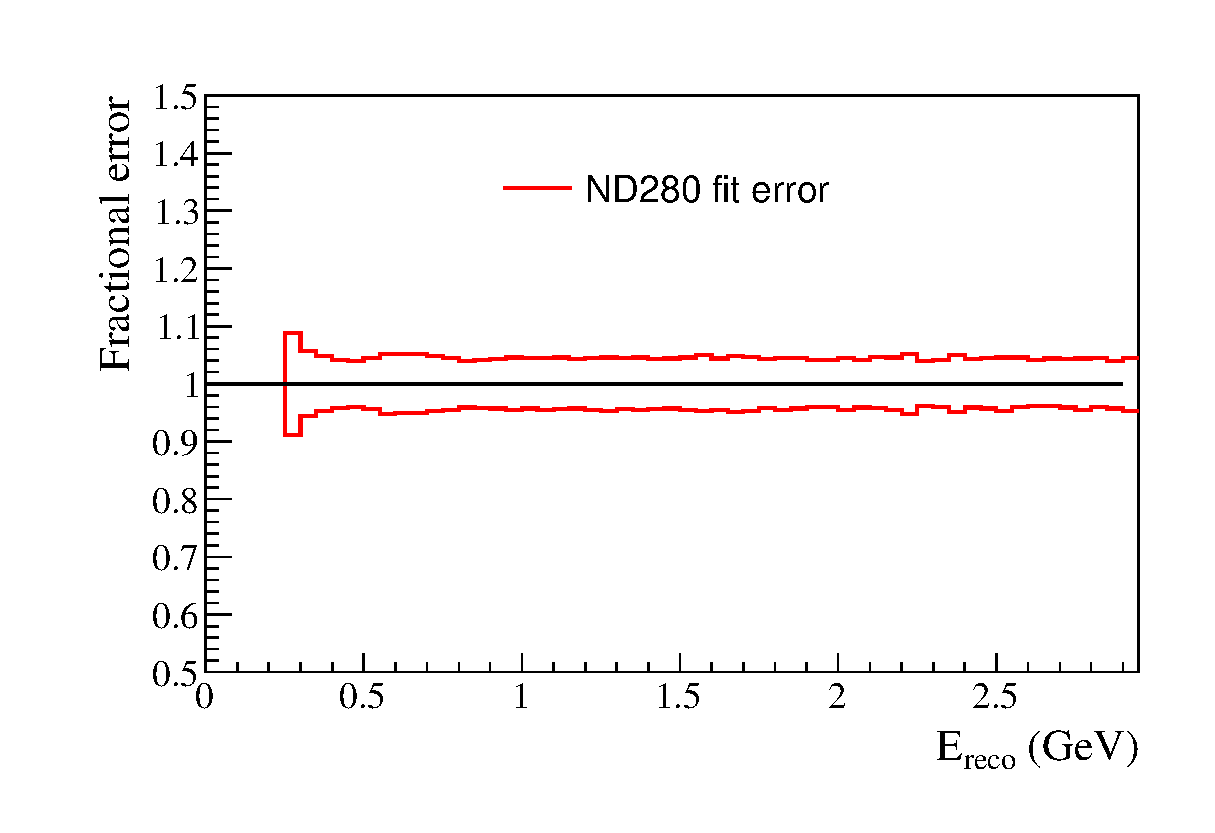
\includegraphics[width=0.9\textwidth]{joint_plots/systematics/Asimov_A_1Rmuoscillated_BANFF_xsec_envelope_ratio.eps} 
\caption{Muon-like, neutrino mode}
\end{subfigure}
%rhc mu-like
\begin{subfigure}[b]{0.49\textwidth} \centering
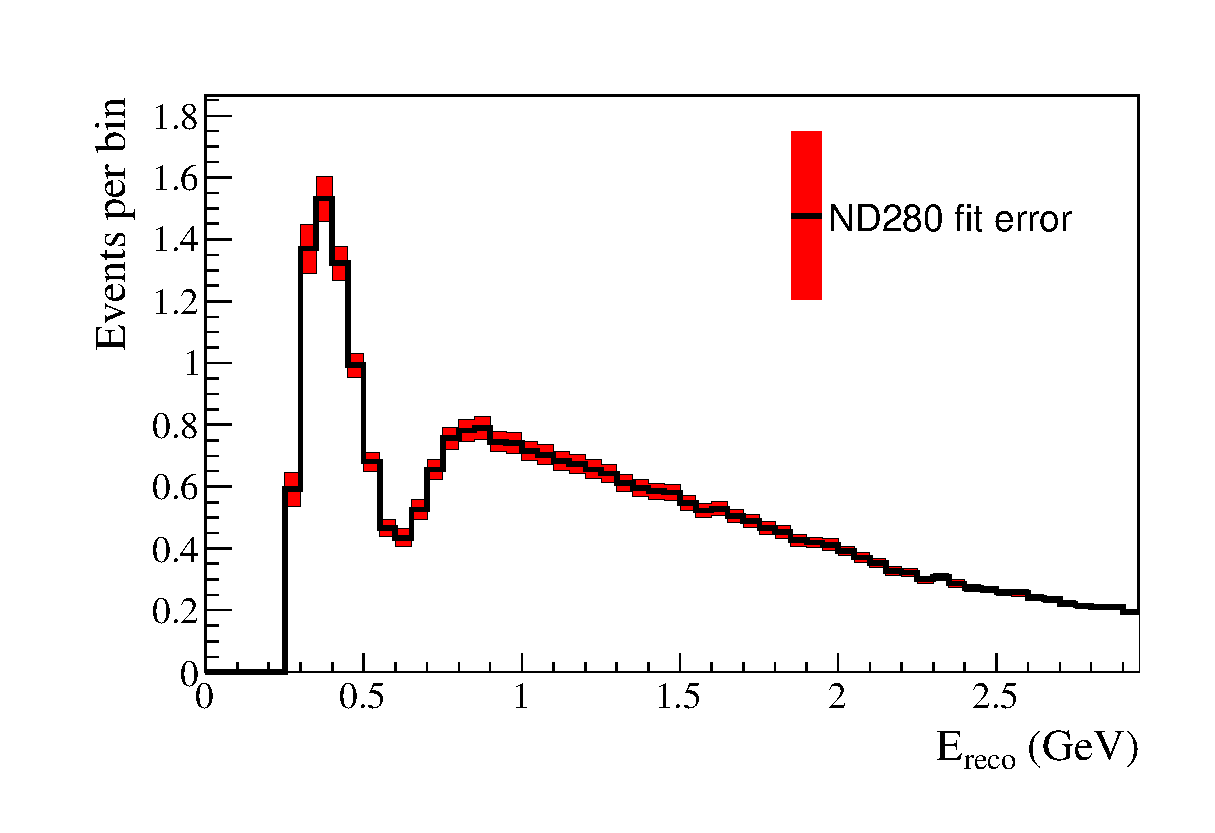
\includegraphics[width=0.9\textwidth]{joint_plots/systematics/Asimov_A_RHC1Rmuoscillated_BANFF_xsec_envelope.eps} \\ 
\caption{Muon-like, antineutrino mode}
\end{subfigure}
\begin{subfigure}[b]{0.49\textwidth} \centering
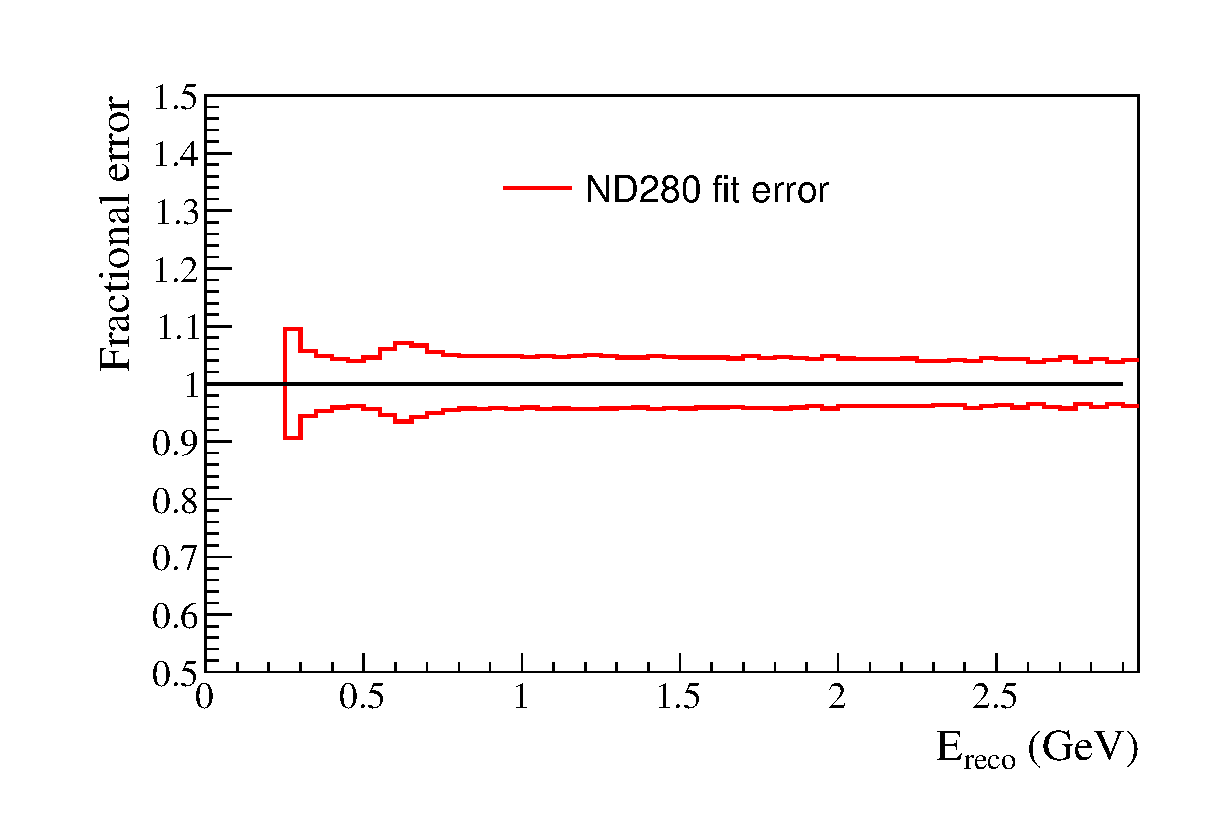
\includegraphics[width=0.9\textwidth]{joint_plots/systematics/Asimov_A_RHC1Rmuoscillated_BANFF_xsec_envelope_ratio.eps} \\ 
\caption{Muon-like, antineutrino mode}
\end{subfigure}
%fhc e-like
\begin{subfigure}[b]{0.49\textwidth} \centering
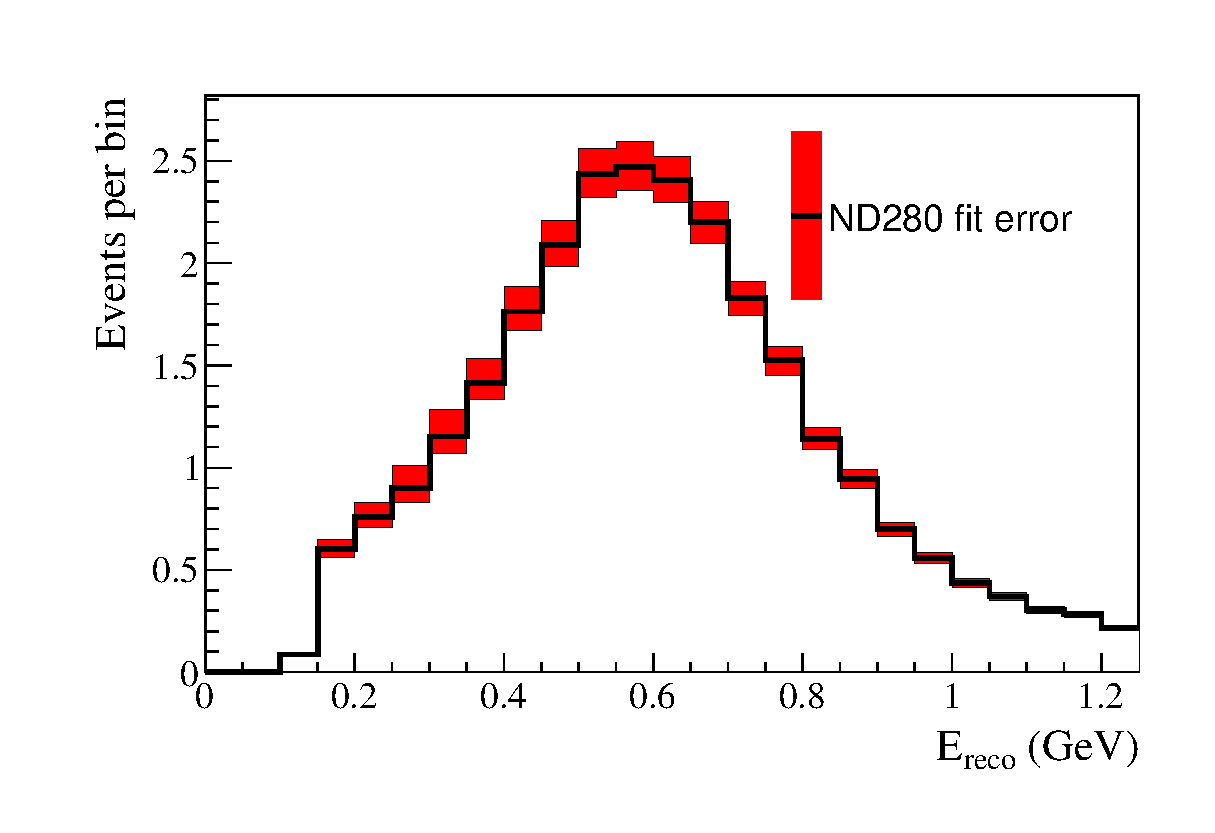
\includegraphics[width=0.9\textwidth]{joint_plots/systematics/Asimov_A_1Reoscillated_BANFF_xsec_envelope.eps} 
\caption{Electron-like, neutrino mode}
\end{subfigure}
\begin{subfigure}[b]{0.49\textwidth} \centering
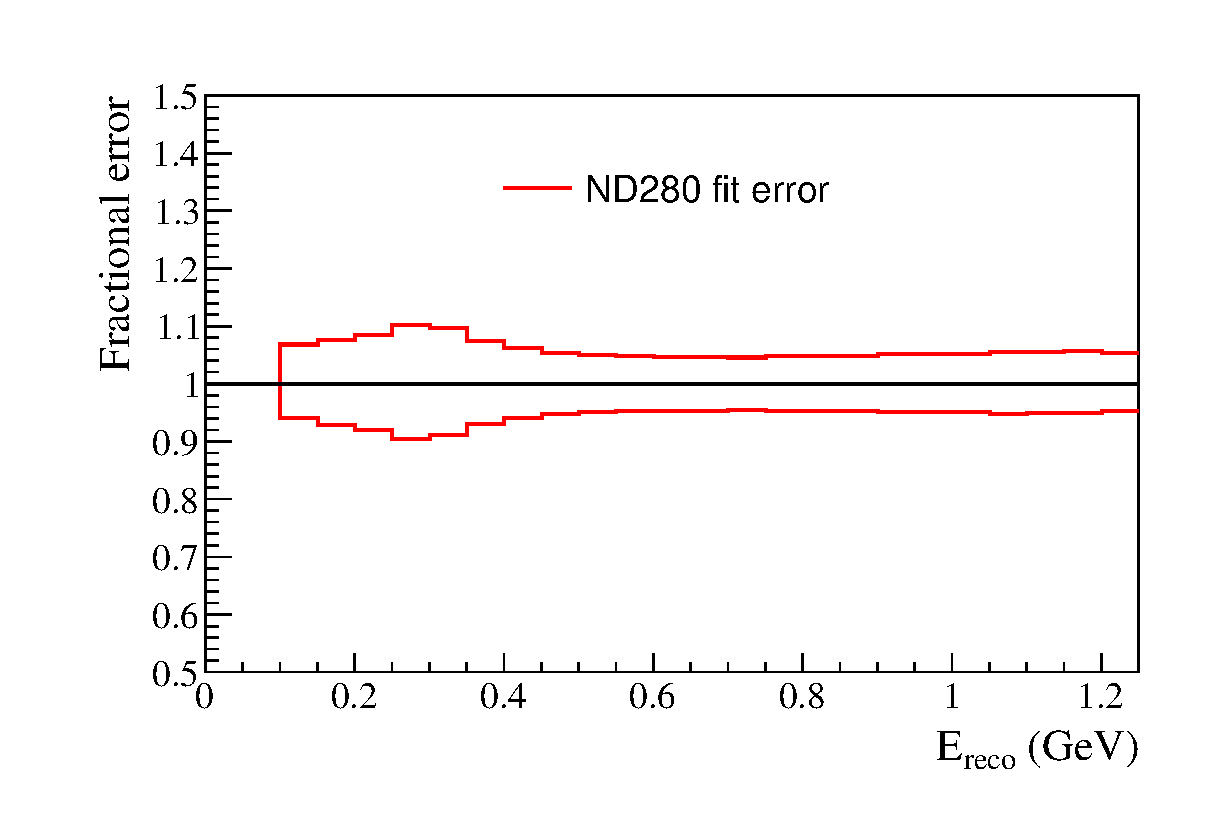
\includegraphics[width=0.9\textwidth]{joint_plots/systematics/Asimov_A_1Reoscillated_BANFF_xsec_envelope_ratio.eps} 
\caption{Electron-like, neutrino mode}
\end{subfigure}
%rhc e-like
\begin{subfigure}[b]{0.49\textwidth} \centering
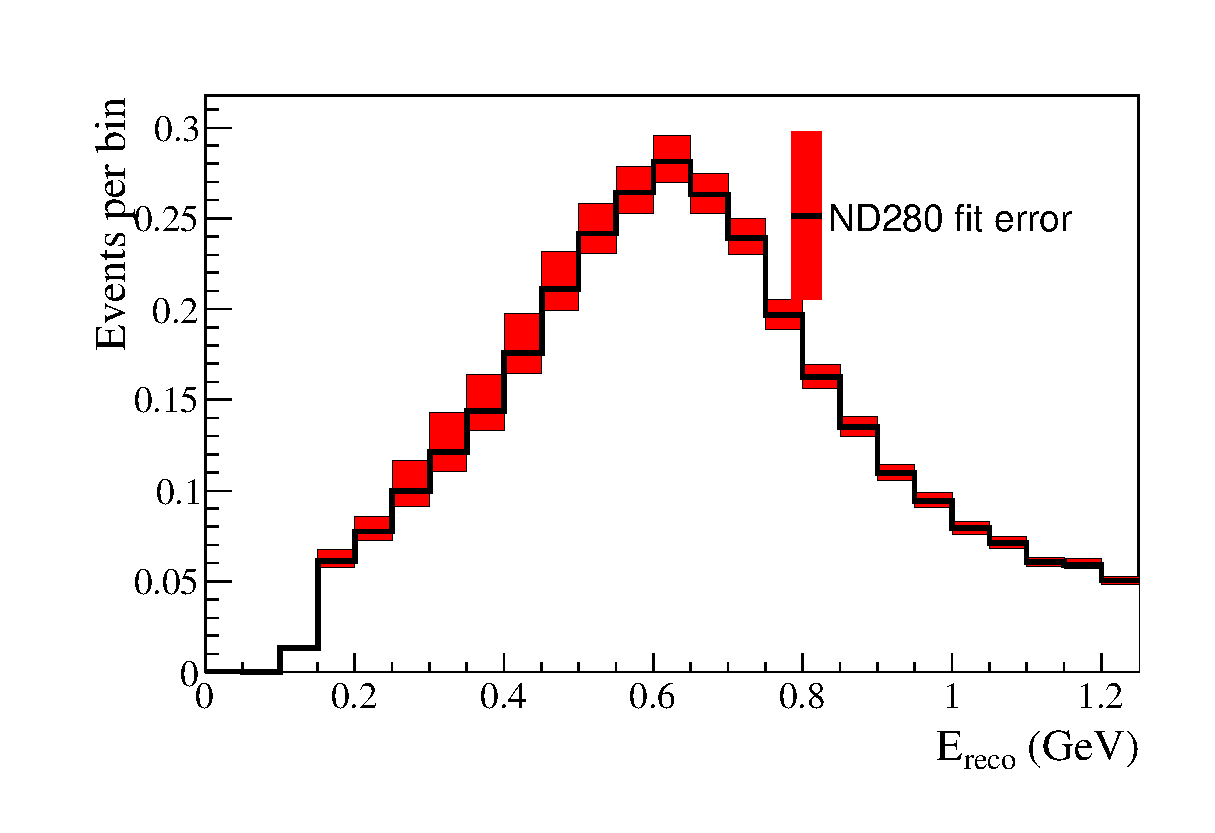
\includegraphics[width=0.9\textwidth]{joint_plots/systematics/Asimov_A_RHC1Reoscillated_BANFF_xsec_envelope.eps} 
\caption{Electron-like, antineutrino mode}
\end{subfigure}
\begin{subfigure}[b]{0.49\textwidth} \centering
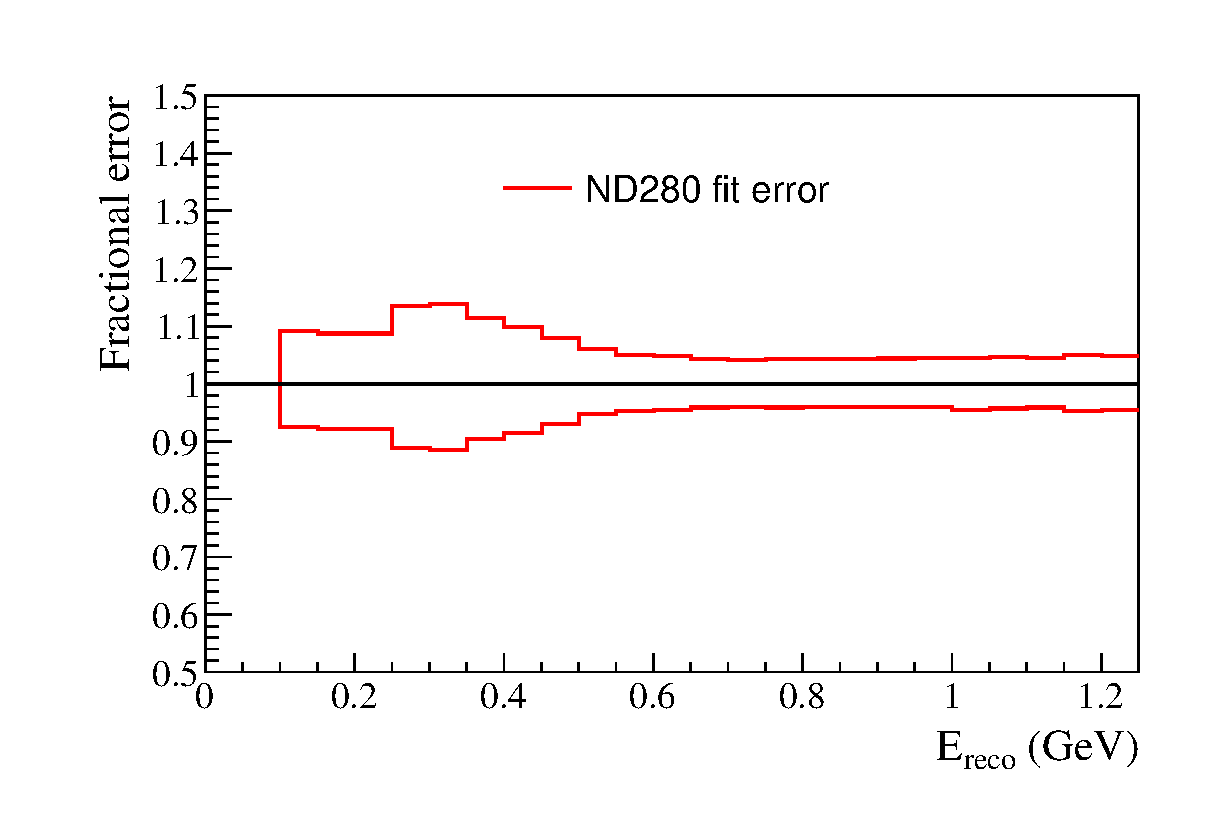
\includegraphics[width=0.9\textwidth]{joint_plots/systematics/Asimov_A_RHC1Reoscillated_BANFF_xsec_envelope_ratio.eps} 
\caption{Electron-like, antineutrino mode}
\end{subfigure}
\caption {
Error envelopes (left) and fractional errors (right) for the reconstructed neutrino energy spectrum
as a result of the cross section systematic parameters. 
10k toy MC experiments are generated for the Asimov data set A shown in \cref{tab:osc_params_joint_asimov}
with randomized systematic parameters, taking into account their correlations.
Since the parameters $\delta_{CP}$, $\theta_{23}$ and $\Delta m^2_{32}$ ($\Delta m^2_{13}$) and mass hierarchy
will be measured,
only the uncertainty on 
$\sin^2 \theta_{13}$,
$\sin^2 \theta_{12}$
and 
$\Delta m^2_{21}$ 
are taken into account.
BANFF tuned MC templates are used. 
The distributions correspond to the collected statistics in the full Run 1-6 data set.
}
\label{fig:xsec_envelope_Asimov_A}
\end{figure*}


\begin{figure*}[htb]
\center
%fhc mu-like
\begin{subfigure}[b]{0.49\textwidth} \centering
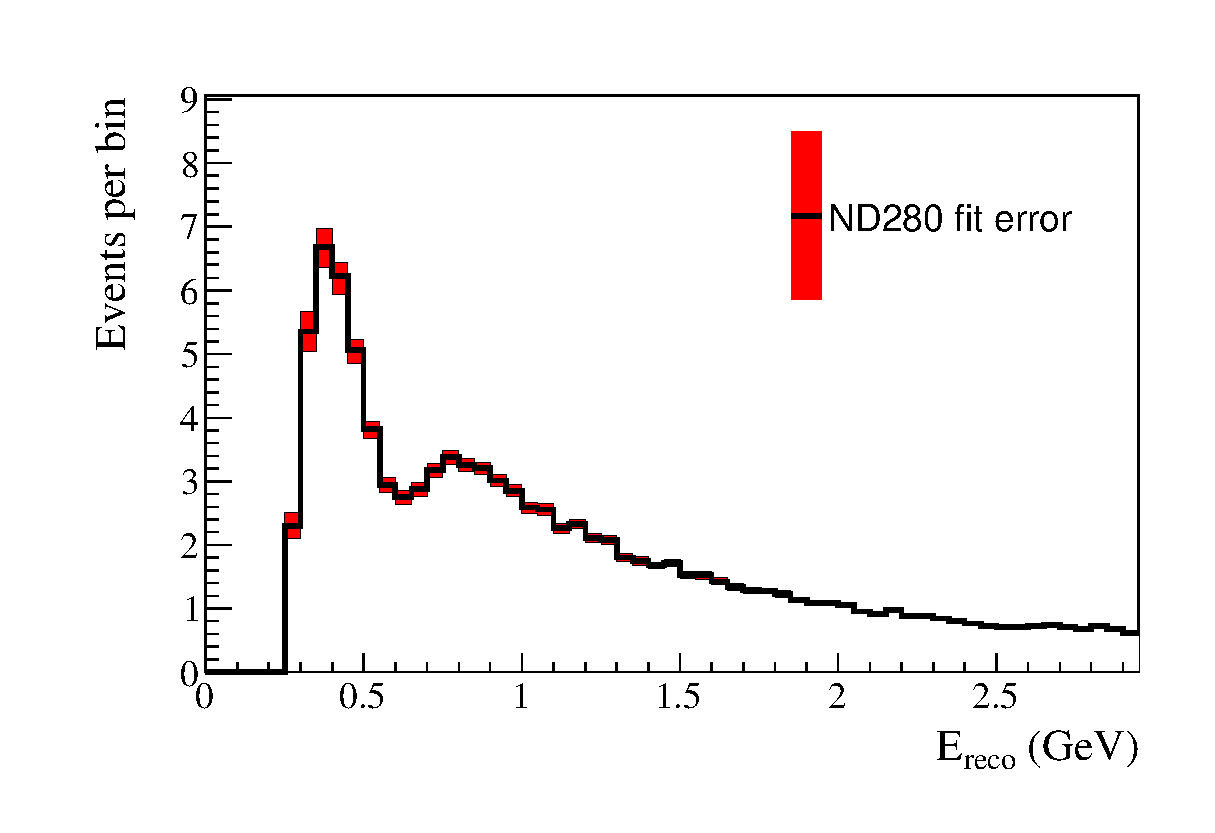
\includegraphics[width=0.9\textwidth]{joint_plots/systematics/Asimov_A_1Rmuoscillated_BANFF_envelope.eps} 
\caption{Muon-like, neutrino mode}
\end{subfigure}
\begin{subfigure}[b]{0.49\textwidth} \centering
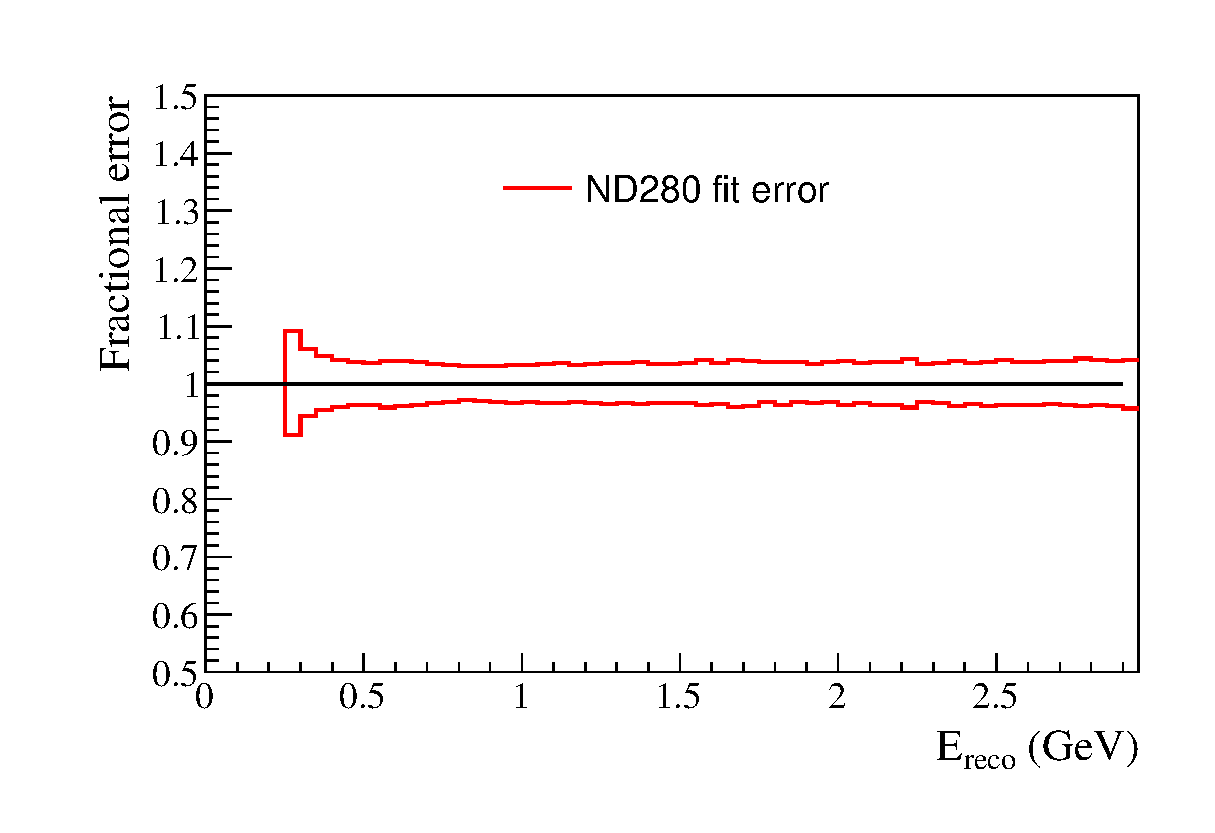
\includegraphics[width=0.9\textwidth]{joint_plots/systematics/Asimov_A_1Rmuoscillated_BANFF_envelope_ratio.eps} 
\caption{Muon-like, neutrino mode}
\end{subfigure}
%fhc mu-like
\begin{subfigure}[b]{0.49\textwidth} \centering
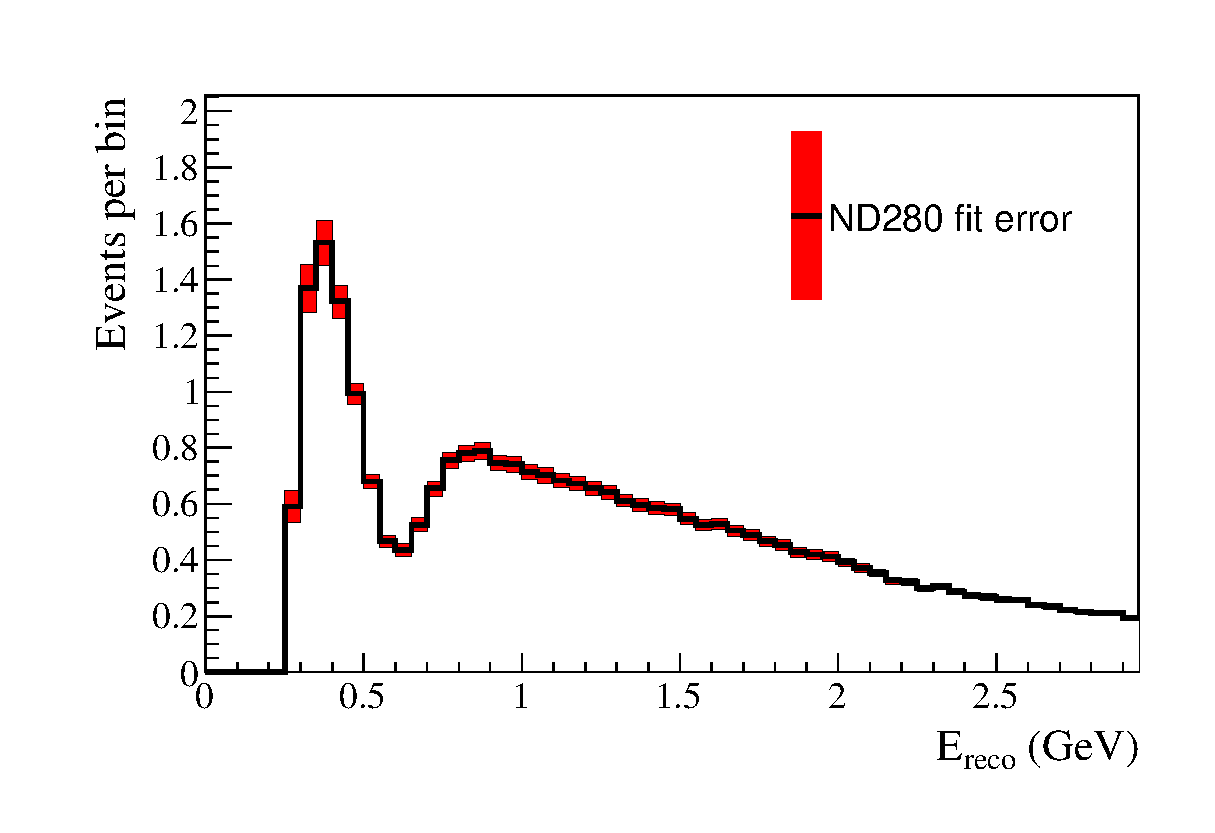
\includegraphics[width=0.9\textwidth]{joint_plots/systematics/Asimov_A_RHC1Rmuoscillated_BANFF_envelope.eps} \\ 
\caption{Muon-like, antineutrino mode}
\end{subfigure}
\begin{subfigure}[b]{0.49\textwidth} \centering
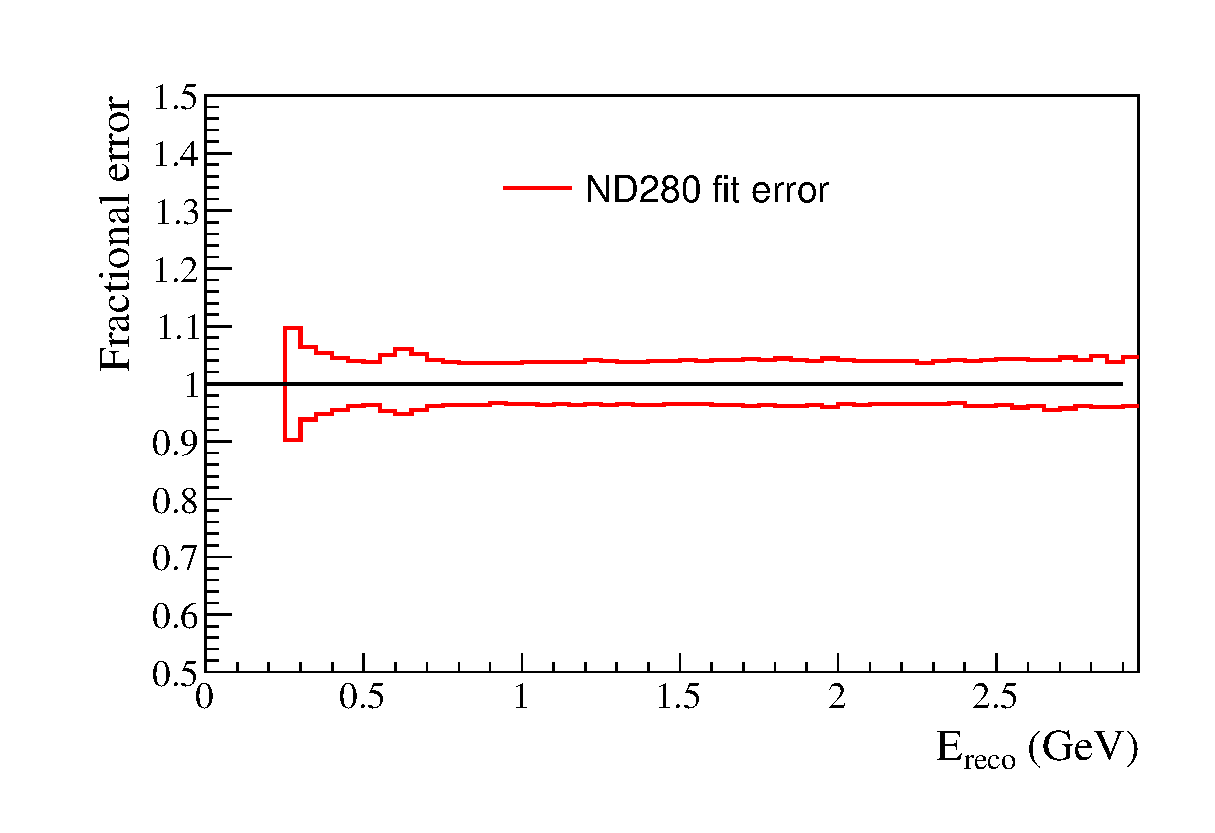
\includegraphics[width=0.9\textwidth]{joint_plots/systematics/Asimov_A_RHC1Rmuoscillated_BANFF_envelope_ratio.eps} \\ 
\caption{Muon-like, antineutrino mode}
\end{subfigure}
%fhc mu-like
\begin{subfigure}[b]{0.49\textwidth} \centering
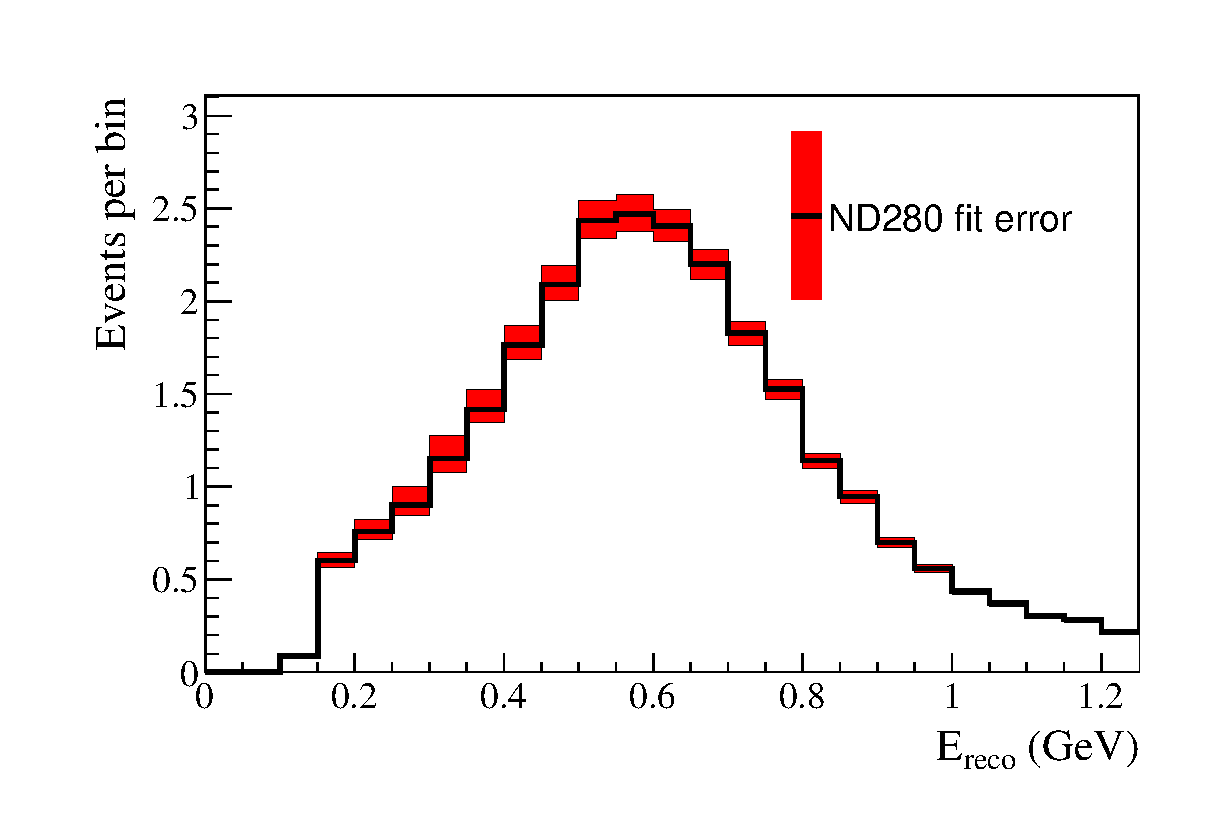
\includegraphics[width=0.9\textwidth]{joint_plots/systematics/Asimov_A_1Reoscillated_BANFF_envelope.eps} 
\caption{Electron-like, neutrino mode}
\end{subfigure}
\begin{subfigure}[b]{0.49\textwidth} \centering
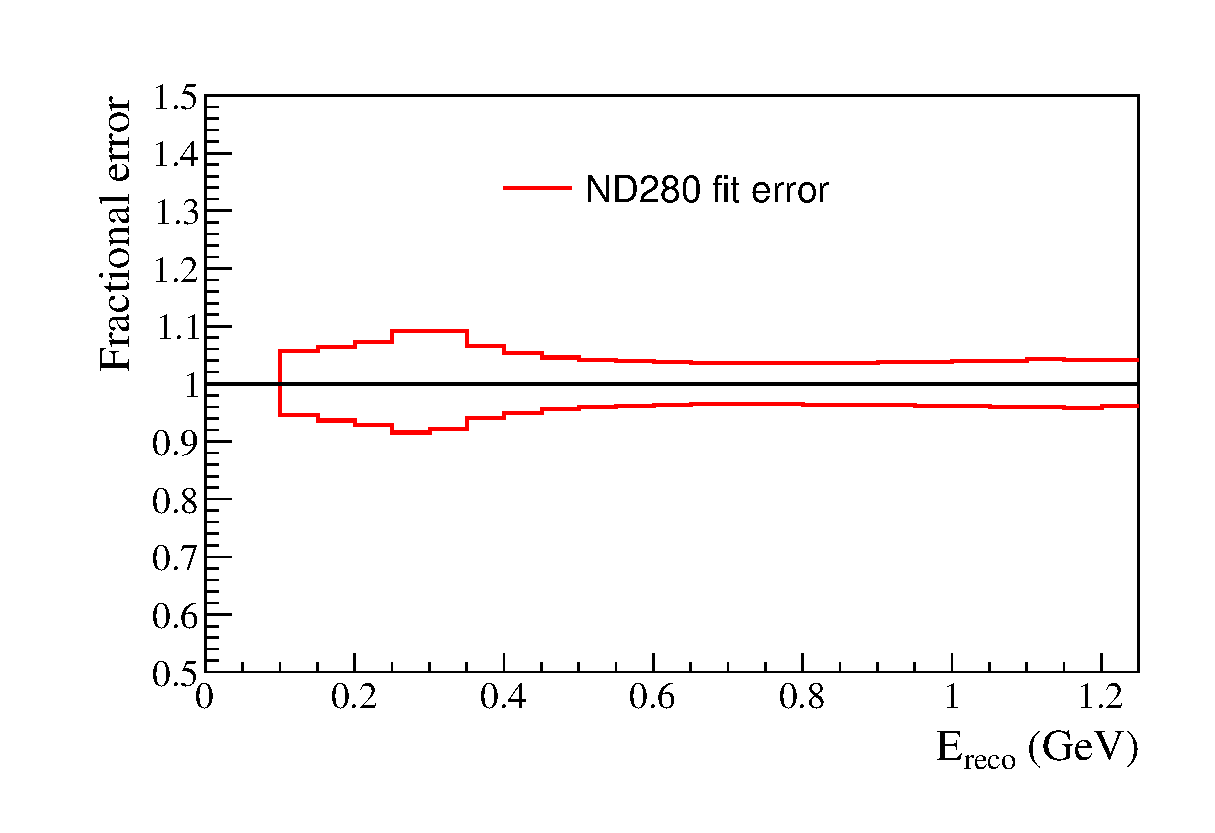
\includegraphics[width=0.9\textwidth]{joint_plots/systematics/Asimov_A_1Reoscillated_BANFF_envelope_ratio.eps} 
\caption{Electron-like, neutrino mode}
\end{subfigure}
%fhc mu-like
\begin{subfigure}[b]{0.49\textwidth} \centering
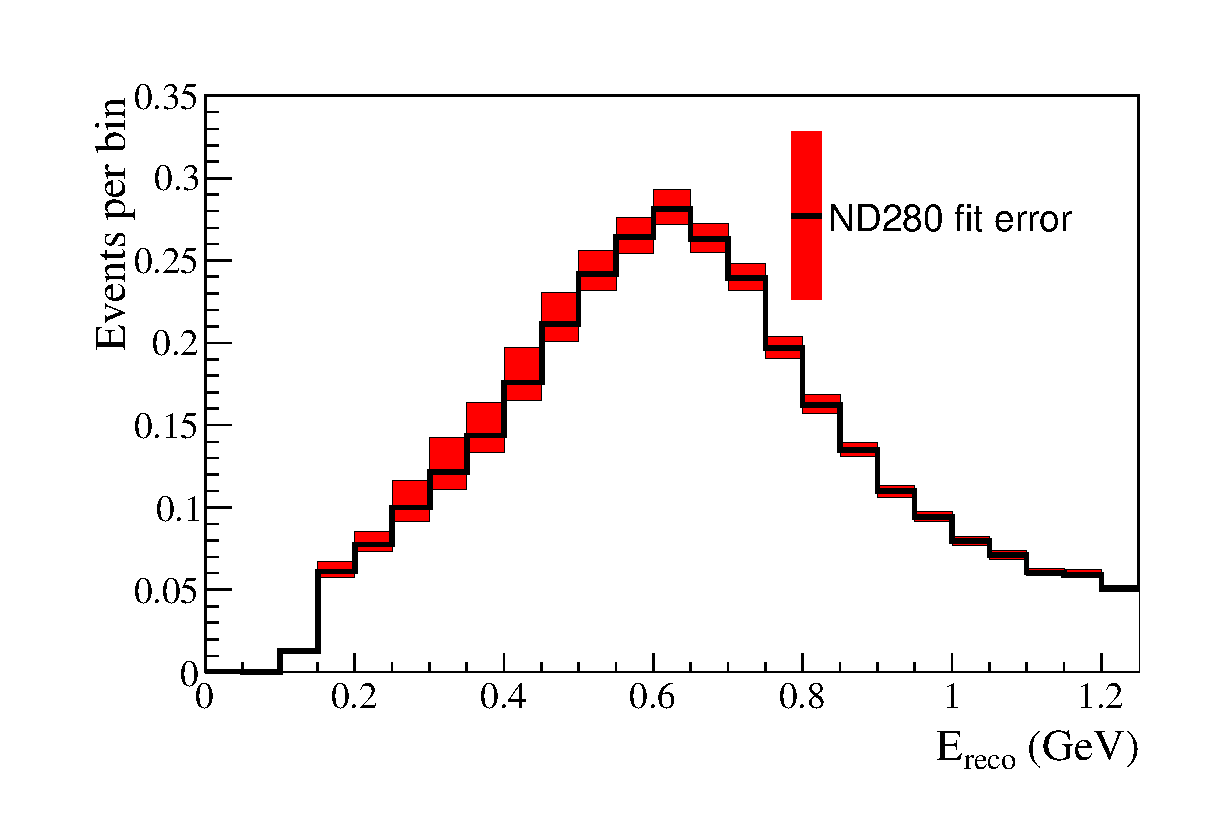
\includegraphics[width=0.9\textwidth]{joint_plots/systematics/Asimov_A_RHC1Reoscillated_BANFF_envelope.eps} 
\caption{Electron-like, antineutrino mode}
\end{subfigure}
\begin{subfigure}[b]{0.49\textwidth} \centering
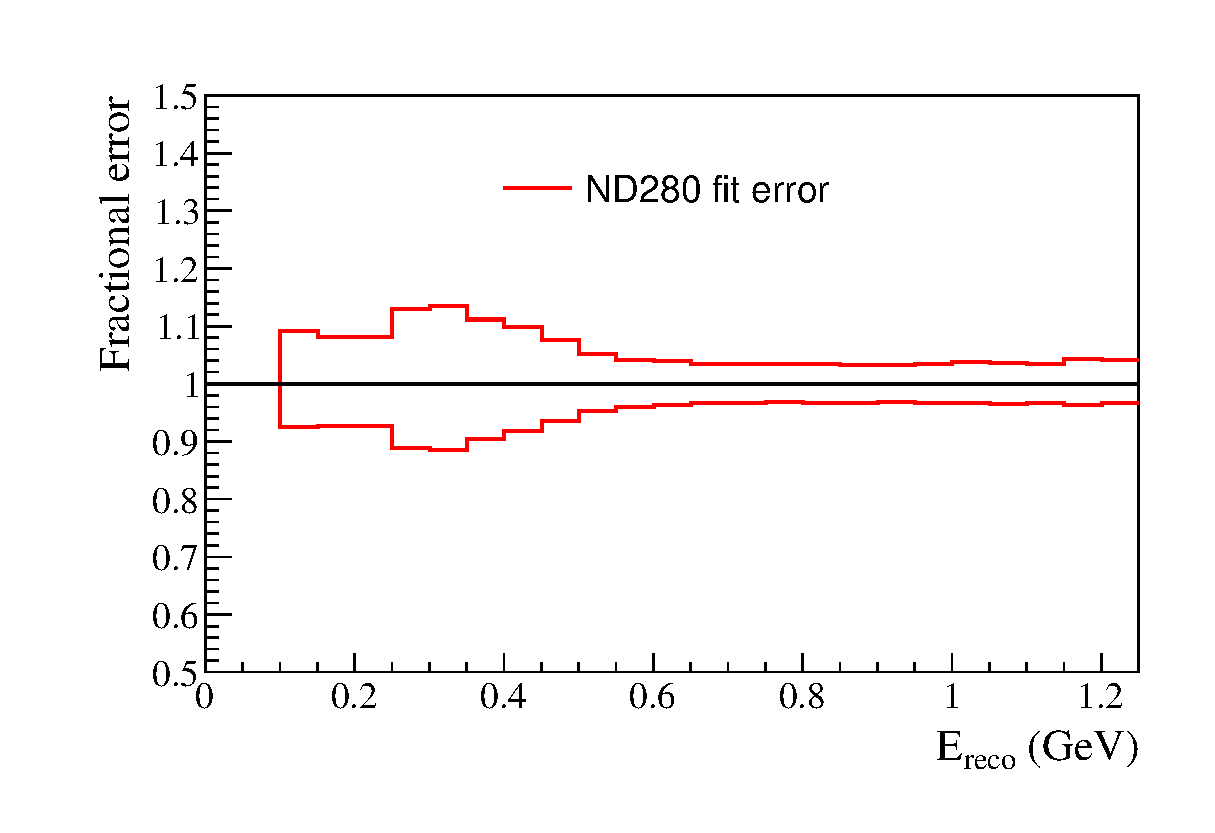
\includegraphics[width=0.9\textwidth]{joint_plots/systematics/Asimov_A_RHC1Reoscillated_BANFF_envelope_ratio.eps} 
\caption{Electron-like, antineutrino mode}
\end{subfigure}
\caption {
Error envelopes (left) and fractional errors (right) for the reconstructed neutrino energy spectrum
as a result of the flux plus cross section systematic parameters. 
10k toy MC experiments are generated for the Asimov data set A shown in \cref{tab:osc_params_joint_asimov}
with randomized systematic parameters, taking into account their correlations.
Since the parameters $\delta_{CP}$, $\theta_{23}$ and $\Delta m^2_{32}$ ($\Delta m^2_{13}$) and mass hierarchy
will be measured,
only the uncertainty on 
$\sin^2 \theta_{13}$,
$\sin^2 \theta_{12}$
and 
$\Delta m^2_{21}$ 
are taken into account.
BANFF tuned MC templates are used. 
The distributions correspond to the collected statistics in the full Run 1-6 data set.
}
\label{fig:flux_xsec_envelope_Asimov_A}
\end{figure*}

\clearpage


%..................

